\documentclass[a4paper,11pt]{book}
%\documentclass[a4paper,twoside,11pt,titlepage]{book}
% ! TEX root = ./proyecto.tex
\usepackage{listings}
\usepackage[utf8]{inputenc}
\usepackage[spanish]{babel}
\usepackage{dirtytalk}
\usepackage{subcaption}
\usepackage{multirow}
\usepackage{adjustbox}
\usepackage{csquotes}
\usepackage[maxnames=50,giveninits=true,backend=bibtex]{biblatex}
\usepackage{float} % Para poner [H] en las imagenes/tablas
\usepackage{algorithm}
\usepackage{algpseudocode}
\usepackage{appendix}

% Cambiar nombre de las tablas de 'Cuadro' a 'Tabla'
\captionsetup[table]{name=Tabla}
% Cambiar el nombre de Algorithm a Algoritmo.
\makeatletter
\renewcommand{\ALG@name}{Algoritmo}
\makeatother

\makeatletter
\def\BState{\State\hskip-\ALG@thistlm}
\makeatother

% \usepackage[style=list, number=none]{glossary} %
%\usepackage{titlesec}
%\usepackage{pailatino}\textbf{}

\decimalpoint
\usepackage{dcolumn}
\newcolumntype{.}{D{.}{\esperiod}{-1}}
\makeatletter
\addto\shorthandsspanish{\let\esperiod\es@period@code}
\makeatother
\usepackage{amsmath,amsfonts,amsthm}
\newcommand{\verticalspace}{\vspace{0.09in}}

%\usepackage[chapter]{algorithm}
\RequirePackage{verbatim}
%\RequirePackage[Glenn]{fncychap}
\usepackage{fancyhdr}
\usepackage{graphicx}
\usepackage{afterpage}

\usepackage{longtable}

\usepackage[pdfborder={000}]{hyperref} %referencia

% ********************************************************************
% Re-usable information
% ********************************************************************
\newcommand{\myTitle}{Título del proyecto\xspace}
\newcommand{\myDegree}{Grado en ...\xspace}
\newcommand{\myName}{Nombre Apllido1 Apellido2 (alumno)\xspace}
\newcommand{\myProf}{Nombre Apllido1 Apellido2 (tutor1)\xspace}
\newcommand{\myOtherProf}{Nombre Apllido1 Apellido2 (tutor2)\xspace}
%\newcommand{\mySupervisor}{Put name here\xspace}
\newcommand{\myFaculty}{Escuela Técnica Superior de Ingenierías Informática y de
Telecomunicación\xspace}
\newcommand{\myFacultyShort}{E.T.S. de Ingenierías Informática y de
Telecomunicación\xspace}
\newcommand{\myDepartment}{Departamento de ...\xspace}
\newcommand{\myUni}{\protect{Universidad de Granada}\xspace}
\newcommand{\myLocation}{Granada\xspace}
\newcommand{\myTime}{\today\xspace}
\newcommand{\myVersion}{Version 0.1\xspace}


\hypersetup{
   pdfauthor = {\myName (email (en) ugr (punto) es)},
   pdftitle = {\myTitle},
   pdfsubject = {},
   pdfkeywords = {palabra_clave1, palabra_clave2, palabra_clave3, ...},
   pdfcreator = {LaTeX con el paquete ....},
   pdfproducer = {pdflatex}
}

%\hyphenation{}


%\usepackage{doxygen/doxygen}
%\usepackage{pdfpages}
\usepackage{url}
\usepackage{colortbl,longtable}
\usepackage[stable]{footmisc}
%\usepackage{index}

%\makeindex
%\usepackage[style=long, cols=2,border=plain,toc=true,number=none]{glossary}
% \makeglossary

% Definición de comandos que me son tiles:
%\renewcommand{\indexname}{Índice alfabético}
%\renewcommand{\glossaryname}{Glosario}

\pagestyle{fancy}
\fancyhf{}
\fancyhead[LO]{\leftmark}
\fancyhead[RE]{\rightmark}
\fancyhead[RO,LE]{\textbf{\thepage}}
\renewcommand{\chaptermark}[1]{\markboth{\textbf{#1}}{}}
\renewcommand{\sectionmark}[1]{\markright{\textbf{\thesection. #1}}}

\setlength{\headheight}{1.5\headheight}

\newcommand{\HRule}{\rule{\linewidth}{0.5mm}}
%Definimos los tipos teorema, ejemplo y definición podremos usar estos tipos
%simplemente poniendo \begin{teorema} \end{teorema} ...
\newtheorem{teorema}{Teorema}[chapter]
\newtheorem{ejemplo}{Ejemplo}[chapter]
\newtheorem{definicion}{Definición}[chapter]

\definecolor{gray97}{gray}{.97}
\definecolor{gray75}{gray}{.75}
\definecolor{gray45}{gray}{.45}
\definecolor{gray30}{gray}{.94}

\lstset{ frame=Ltb,
     framerule=0.5pt,
     aboveskip=0.5cm,
     framextopmargin=3pt,
     framexbottommargin=3pt,
     framexleftmargin=0.1cm,
     framesep=0pt,
     rulesep=.4pt,
     backgroundcolor=\color{gray97},
     rulesepcolor=\color{black},
     %
     stringstyle=\ttfamily,
     showstringspaces = false,
     basicstyle=\scriptsize\ttfamily,
     commentstyle=\color{gray45},
     keywordstyle=\bfseries,
     %
     numbers=left,
     numbersep=6pt,
     numberstyle=\tiny,
     numberfirstline = false,
     breaklines=true,
   }
 
% minimizar fragmentado de listados
\lstnewenvironment{listing}[1][]
   {\lstset{#1}\pagebreak[0]}{\pagebreak[0]}

\lstdefinestyle{CodigoC}
   {
	basicstyle=\scriptsize,
	frame=single,
	language=C,
	numbers=left
   }
\lstdefinestyle{CodigoC++}
   {
	basicstyle=\small,
	frame=single,
	backgroundcolor=\color{gray30},
	language=C++,
	numbers=left
   }

 
\lstdefinestyle{Consola}
   {basicstyle=\scriptsize\bf\ttfamily,
    backgroundcolor=\color{gray30},
    frame=single,
    numbers=none
   }


\newcommand{\bigrule}{\titlerule[0.5mm]}

%Para conseguir que en las páginas en blanco no ponga cabecerass
\makeatletter
\def\clearpage{%
  \ifvmode
    \ifnum \@dbltopnum =\m@ne
      \ifdim \pagetotal <\topskip
        \hbox{}
      \fi
    \fi
  \fi
  \newpage
  \thispagestyle{empty}
  \write\m@ne{}
  \vbox{}
  \penalty -\@Mi
}
\makeatother

\usepackage{pdfpages}
\addbibresource{bibliografia/bibliografia.bib}

\begin{document}
\begin{titlepage}
 
 
\newlength{\centeroffset}
\setlength{\centeroffset}{-0.5\oddsidemargin}
\addtolength{\centeroffset}{0.5\evensidemargin}
\thispagestyle{empty}

\noindent\hspace*{\centeroffset}\begin{minipage}{\textwidth}

\centering

\includegraphics[width=0.9\textwidth]{imagenes/logo_ugr.jpg}\\[1.4cm]

\textsc{ \Large TRABAJO FIN DE MÁSTER\\[0.2cm]}
\textsc{ MÁSTER EN CIENCIAS DE DATOS E INGENIERÍA DE COMPUTADORES}\\[1cm]
% Upper part of the page
% 
% Title
{\large\bfseries Algoritmos de Deep Learning para el tratamiento de series temporales de clasificación\\
}
\noindent\rule[-1ex]{\textwidth}{3pt}\\[3.5ex]

\end{minipage}

\vspace{2.5cm}
\noindent\hspace*{\centeroffset}\begin{minipage}{\textwidth}
\centering

\textbf{Autor}\\ {Alberto Armijo Ruiz}\\[2.5ex]
\textbf{Director}\\
{Salvador García López}\\[2cm]

\includegraphics[width=0.3\textwidth]{imagenes/etsiit_logo.png}\\[0.1cm]
\textsc{Escuela Técnica Superior de Ingenierías Informática y de Telecomunicación}\\
\textsc{---}\\
\today
\end{minipage}
%\addtolength{\textwidth}{\centeroffset}
%\vspace{\stretch{2}}
\end{titlepage}



\chapter*{}
%\thispagestyle{empty}
%\cleardoublepage

%\thispagestyle{empty}





\cleardoublepage
\thispagestyle{empty}

\begin{center}
{\large\bfseries Algoritmos de Deep Learning para el tratamiento de series temporales de clasificación}\\
\end{center}
\begin{center}
Alberto Armijo Ruiz\\
\end{center}

%\vspace{0.7cm}
\noindent{\textbf{Palabras clave}: LSTM, Deep Learning, Ciencia de Datos, Series Temporales, Clasificación, Desbalanceo de clases, Oversampling.\\

\vspace{0.7cm}
\noindent{\textbf{Resumen}}\\

Actualmente la Ciencia de Datos es una de las áreas de estudio que más repercusión está causando, dentro de esta, el Deep Learning es uno de los campos más famosos.\newline

Hoy en día existen estudios específicos sobre Series Temporales de Clasificación, pero no existe ningún estudio sobre la aplicación generalista del Deep Learning a casos de estudio estándar de Series Temporales de Clasificación. Por ello el objetivo de este trabajo será estudiar la aplicación del Deep Learning a las Series Temporales de Clasificación con desbalanceo de clases.\newline 

Este estudio utilizará ocho conjuntos de datos sobre Series Temporales de Clasificación con diferentes grados de desbalanceo de clases. A estos se aplicarán SMOTE, ADASYN y MWMOTE para realizar oversampling, existen otras técnicas que se han estudiado como el undersampling o el peso de clases pero no se han utilizan dentro del estudio. También se utiliza el algoritmo Boruta como método de selección de características, existen otras características como selección de características con Chi-Cuadrado pero Boruta ofrece un buen rendimiento de forma general.\newline

A parte de los métodos anteriores, se estudiará el uso de una ventana de diferentes tamaños para aprovechar la dependencia temporal con la que cuentan la series temporales intentando replicar el comportamiento de modelos de predicción de series temporales clásicos para mejorar los resultados iniciales.\newline 

Para la predicción se hará uso de las LSTM, uno de los tipos de red neuronal más utilizados en la actualidad; además de este, se utilizarán otros modelos que se encuentran en el estado del arte de la clasificación como son SVM, RandomForest y XGBoost y se comparán los resultados obtenidos.\newline

\cleardoublepage


\thispagestyle{empty}


\begin{center}
{\large\bfseries Deep Learning algorithms for time series classification}\\
\end{center}
\begin{center}
Alberto Armijo Ruiz \\
\end{center}

%\vspace{0.7cm}
\noindent{\textbf{Keywords}: LSTM, Deep Learning, Data Science, Time Series, Classification, Class Imbalance, Oversampling.}\\

\vspace{0.7cm}
\noindent{\textbf{Abstract}}\\

Currently Data Science is one of the areas of study that is causing more impact, within this, Deep Learning is one of the most famous fields. \newline

Nowadays there are specific studies on Time Series Classification, but there is no study on the generalist application of Deep Learning to standard case studies of Time Series Classification. Therefore, the objective of this paper will be to study the application of Deep Learning to Classification Time Series with class imbalance.\newline

This study will use eight datasets of Time Series Classification problems with different degrees of class imbalance. To these will be applied SMOTE, ADASYN and MWMOTE to perform oversampling, there are other techniques that have been studied as undersampling or class-weight but have not been used within the study. The Boruta algorithm is also used  as a method of feature selection, there are other features such as feature selection with Chi-Square but Boruta offers good performance overall.\newline

Apart from the previous methods, we will study the use of a window of different sizes to take advantage of the time dependency of the time series trying to replicate the behavior of classic time series models to improve the initial results.\newline

For the prediction, use will be made of LSTM, one of the most commonly used neural network types at present; in addition to this, other state of the art models for classification will be used, such as SVM, RandomForest and XGBoost, and the results obtained will be compared.\newline


\chapter*{}
\thispagestyle{empty}

\noindent\rule[-1ex]{\textwidth}{2pt}\\[4.5ex]

D. \textbf{Salvador García López}, Profesor del Área de Soft Computing and Intelligent Information Systems del Departamento DECSAI de la Universidad de Granada.

\vspace{0.5cm}

\textbf{Informan:}

\vspace{0.5cm}

Que el presente trabajo, titulado \textit{\textbf{Algoritmos de Deep Learning para el tratamiento de series temporales de clasificación}},
ha sido realizado bajo su supervisión por \textbf{Alberto Armijo Ruiz}, y autorizamos la defensa de dicho trabajo ante el tribunal
que corresponda.

\vspace{0.5cm}

Y para que conste, expiden y firman el presente informe en Granada a 12 de Agosto de 2019 .

\vspace{1cm}

\textbf{Los directores:}

\vspace{5cm}

\noindent \textbf{Salvador García López}



%\frontmatter
\tableofcontents
%\listoffigures
%\listoftables
%
%\mainmatter
%\setlength{\parskip}{5pt}
\chapter{Introducción}
\section{Objetivos}
Los objetivos propuesto para este Trabajo Fin de Máster son los siguientes:

\begin{itemize}
	\item Estudio de algoritmos básicos para series temporales y clasificación, tratamiento de series temporales de clasificación.
	\item Estudio sobre problema de desbalanceo de clases, métodos para tratar con desbalanceo, centrándose en el estudio de técnicas de oversampling utilizadas actualmente, métricas utilizadas para este tipo de problema.
	\item Estudio sobre LSTM y aplicación de estas al problemas de clasificación.
	\item Realización de pruebas sobre un conjunto de datasets de series temporales de clasificación con desbalanceo de clases, comparación y análisis de los resultados obtenidos por los diferentes modelos.
	\item Obtener conclusiones y trabajos futuros.
\end{itemize}
\newpage
\section{Motivación}
A día de hoy, la minería de datos en series temporales son un tipo de problema en auge. La Clasificación de Series Temporales (TSC, Time Series Classification en Inglés) es una de las áreas donde más investigación se está realizando en los últimos años debido a su gran número de aplicaciones en diferentes sectores como la industria, salud o transporte \cite{cao2013integrated} \cite{cao2014parsimonious} \cite{he2017uncertainty} \cite{xu2018spatio} \cite{roychoudhury2017cost} \cite{liang2013effective} \cite{geng2018cost} . Obtener una buena precisión en este tipo de problema puede ofrecer grandes beneficios por lo que existe un gran interés en este área.\newline

La Clasificación de Series Temporales tiene como objetivo clasificar datos durante el tiempo basado en su comportamiento. Por ejemplo, clasificar el comportamiento de un servidor durante el tiempo puede ayudar a detectar anomalías y a que la resolución de cualquier problema asociado a una anomalía sea más rápido.\newline

El desbalanceo de clases es un problema asociado a la clasificación y muy común en problemas de la vida real. La mayoría de los algoritmos clásicos suelen trabajar sobre la suposición de que el número de datos de cada clase están balanceados, por lo que el desbalanceo entre las diferentes clases hace que el rendimiento de estos algoritmos sea pobre. Esto hace que cuando la clase minoritaria es aquella que tiene más interés en clasificar, como por ejemplo detección de un terremoto; se necesite buscar una solución.\newline

Existen diferentes soluciones para intentar abordar el problema de desbalanceo entre clases a diferentes niveles: a nivel de datos, a nivel del algoritmo o combinaciones de estas dos. Los métodos que abordan el problema a nivel de datos intentan restablecer el balance entre clases mediante el muestreo de datos, añadiendo datos de la clase minoritaria (oversampling), eliminando datos de la clase mayoritaria (undersampling) o una combinación de ambos. Los métodos que abordan el problema a nivel del algoritmo enfatizan en la clase minoritaria manipulando e incorporando diferentes parámetros como el peso de cada clase.\newline

Por otro lado, las redes neuronales son unos de los modelos más famosos actualmente \cite{chung2015gated} \cite{cho2014properties} \cite{karim2017lstm} \cite{swapna2018automated} y se utilizan en un gran número diferentes de problemas obteniendo buenos resultados. Las redes formadas por LSTM (Long Short Term Memory) son un tipo de red que se utiliza en un gran número de problemas de gran complejidad como es la toma de decisiones en videojuegos, reconocimiento del habla o traducción de textos. Este tipo de redes son especialmente buenas en problemas donde hay que procesar secuencias de datos, como  es el caso de las series temporales. Además, la redes neuronales son capaces de trabajar con datos con alta dimensionalidad obteniendo buenos resultados a diferencia de otros métodos de minería de datos clásicos.\newline

En este trabajo se utilizarán diferentes conjuntos de datos sobre Clasificación de Series Temporales. Los conjuntos de datos utilizados de clasificación binaria y contienen desbalanceo entre las clases. Para el procesamiento de dichos conjuntos de datos se utilizará una red de LSTM y diferentes métodos de procesamiento para intentar obtener un buen rendimiento.\newline

Para paliar el desbalanceo de clases se utilizarán métodos de oversampling, en concreto SMOTE; este algoritmo es uno de los más utilizados para oversampling y suele ofrecer buenos resultados. Los resultados obtenidos se compararán con algoritmos clásicos de Machine Learning como por ejemplo SVM.
\newpage

\section{Organización de la memoria}
La memoria de este TFM se organizará en ocho capítulos. En el primer capítulo se mostrarán los objetivos de este trabajo y se describirá la motivación para su realización.\newline

El segundo capítulo trata sobre antecedentes, métodos de clásificación clásicos y métodos de predicción de series temporales, teoría básica sobre funcionamiento de LSTMs y algunas aplicaciones, por último, teoría sobre el problema de desbalanceo de clases.\newline

El tercer, cuarto y quinto capítulo describen tanto métodos de preprocesamiento, funcionamiento de métodos de oversampling que se utilizarán en el estudio, características específicas al preprocesar series temporales de clasificación  como implementación de una red de LSTMs para clasificación.\newline

El sexto capítulo contiene la información sobre los datos que se utilizan en el estudio, la arquitectura de la red básica que se utilizará y medidas para evaluar el rendimiento de la red. El capítulo siete contiene los resultados de las pruebas realizadas y un análisis sobre estos. Por último, el capítulo ocho contiene las conclusiones obtenidas por el estudio.
\chapter{Antecedentes}
En este capítulo se describirán los aspectos generales de los principales componentes del estudio. Primero se describirán diferentes algoritmos básicos usados para clasificación de series temporales. Tras esto se explicarán qué son las LSTM, su funcionamiento y estructura. Por último, se describirá el problema de desbalanceo de clases y diferentes enfoques para solucionarlo.\newline

\section{Clasificación de series temporales. Algoritmos Básicos}
\newpage
\section{LSTM}
Las LSTM ( Long Short-Term Memory ) son un tipo de red neuronal recurrente; este tipo de red es capaz de procesar de procesar secuencias de datos, como por ejemplo vídeos o frases. Este tipo de red neuronal se inventaron para ser usadas en problemas donde la información que se procesa es dependiente de información anteriormente procesada, y esta relación debe ser recordada hasta que deje de ser útil. Actualmente las redes con LSTM se utilizan en diversas tareas, como por ejemplo reconocimiento del habla, traducción, etc.\newline

Una unidad de LSTM o una neurona de LSTM tiene la siguiente estructura:
\begin{itemize}
	\item Puerta de entrada.
	\item Puerta de salida.
	\item Puerta de olvido.
	\item Célula.
\end{itemize}
\vspace{0.09in}
La célula es la encargada de almacenar información; el valor de la célula depende de los valores de las puertas de entrada, salida y olvido. Además, los valores de dichas puertas van cambiando en cada instante de tiempo. En la siguiente imagen se puede ver una representación de las estructura de una LSTM.\newline

\begin{figure}[h]
	\centering
	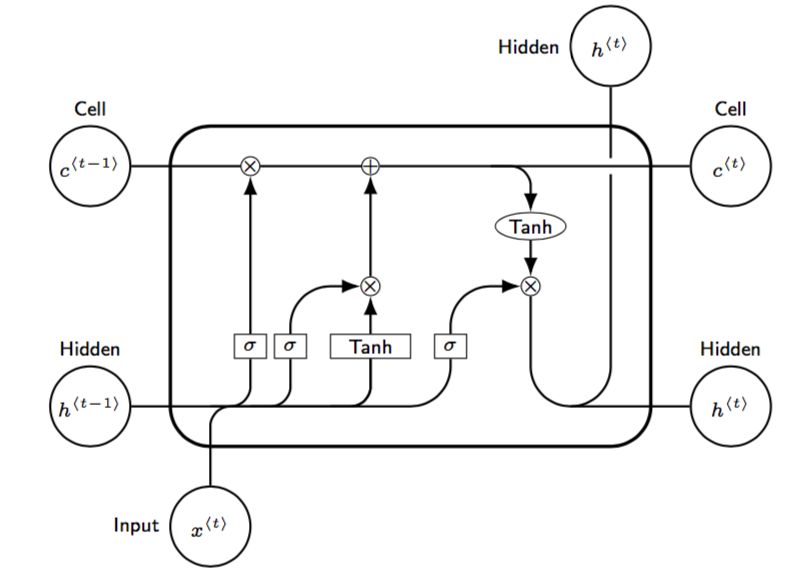
\includegraphics[width=120mm]{imagenes/lstm-struct.png}
	\label{fig:1}
	\caption{Estructura de una LSTM.}
\end{figure}
\vspace{0.09in}
La puerta de olvido tiene como función olvidar información anterior dependiendo de la información actual, dicha función podría expresarse de la siguiente forma.

$$ f^{(t)} = \sigma( W_f[h^{(t-1)}, x(t)] + b_f) $$

Donde:
\begin{itemize}
	\item $x^{(t)}$: entrada de la puerta en el momento $t$.
	\item $h^{(t-1)} $: valor de la salida de la célula en el instante anterior.
	\item $W_f $: matriz de pesos de la puerta de olvido.
	\item $b_f $: sesgo de la puerta de olvido.
	\item $\sigma$: función de activación (valores entre 0 y 1) de la puerta de olvido.
\end{itemize}
\vspace{0.09in}
La puerta de entrada tiene como función aprender los parámetros de entrada para su composición con el estado de la LSTM. PAra ello se debe calcular el estado de la LSTM y seleccionar la información que se utilizará para actualizar el estado. Esto se puede expresar mediante las siguientes funciones:\newline
$$ i^{(t)} = \sigma(W_i[h^{(t-1)}, x^{(t)}] + b_i) $$
$$ s'^{(t)} = \tanh(W_s[h^(t-1), x^{(t)}] + b_s) $$

Donde:
\begin{itemize}
	\item $s'^{(t)}$:estado local de la LSTM, sin tener en cuenta el estado anterior.
	\item $W_i$: matriz de pesos de la puerta de entrada.
	\item $W_s$: matriz de pesos del estado de la LSTM.
	\item $b_i $: sesgo de la puerta de entrada.
	\item $b_s$: sesgo del estado.
\end{itemize}
\verticalspace
Tras esto, se calcula el nuevo estado de la LSTM de la siguiente forma:\newline
$$ s^{(t)} = f^{(t)}s^{(t-1)} + i^{(t)} s'^{(t)} $$
De esta forma, el estado se forma con una parte del estado anterior, la que no se olvida; y con la composición de la entrada con el estado local ( $s'^{(t)}$ ).
\verticalspace

La puerta de salida es la encargada de aprender los parámetros de salida, esto puede expresarse mediante la siguiente función:\newline
$$ o^{(t)} = \sigma(W_o[h^{(t-1)}, x^{(t)}] + b_o) $$
Por último, la salida se calcula como:\newline
$$h^{(t)} = o^{(t)}\tanh(s^{(t)}) $$

La función para calcular la salida puede ser otra, como ReLu; las funciones de activación de las puertas también pueden ser otras.\newline

Como puede verse, las LSTM son capaces de guardar información relevante durante un largo periodo de tiempo y eliminar la información poco importante; por ello, son muy utilizadas en problemas con series temporales, ya que la información en un momento t es dependiente de la información que había en instantes anteriores y las LSTMs son capaces de detectar dicha dependencia y aprenderla.\newline

Las LSTM son un tipo de red recurrente, por lo que se pueden construir arquitecturas basadas en una LSTM que procesa la secuencia de izquierda a derecha y otra de derecha a izquierda; a estas estructuras se les llama LSTM bidireccionales, en la siguiente imagen se muestra un ejemplo de esta estructura.\newline
\newpage

\begin{figure}[h]
	\centering
	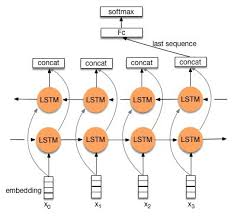
\includegraphics[width=85mm]{imagenes/bidi-lstm.jpg}
	\label{fig:2}
	\caption{Ejemplo de estructura de LSTM bidireccional.}
\end{figure}
\verticalspace
Gracias a este tipo de estructuras pueden resolverse problemas donde la importancia/sentido de un dato no depende de datos anteriores sino por información posterior; por ejemplo, el significado de una palabra puede ser diferente dependiendo de las palabras siguientes que haya en una secuencia y no en las anteriores.
\newpage
\section{Clasificación con clases no balanceadas}
El problema de desbalanceo de clases es un tipo de problema que aparece en problemas de clasificación. el desbalanceo de clases ocurre cuando el número de elementos de una clase es mucho mayor que el número de elementos de la otra clase; a esta clase se le llama clase minoritaria. En la siguiente imagen se puede ver un ejemplo en 2D de un problema de desbalanceo de clases.\newline

\begin{figure}[h]
	\centering
	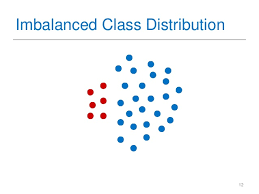
\includegraphics[width=85mm]{imagenes/imbalance_class.png}
	\label{fig:3}
	
\end{figure}
\verticalspace

El principal problema que tiene el desbalanceo de clases es que afecta a la capacidad de aprendizaje de la mayoría de los modelos de minería de datos actuales, exceptuando algunos como los árboles de decisión, aunque también trabajan mejor si no hay desbalanceo. Además, si el desbalanceo es muy grande es posible que los modelos no aprendan directamente la clase minoritaria.\newline

Otro problema es que afecta a las medidas utilizadas normalmente en problemas de clasificación como es el Accuracy; esta medida representa el número de elementos bien clasificados sobre el total de elementos; si por ejemplo la clase minoritaria representa el 0.1\% de los datos y un clasificador predijera todos los datos como elementos de la clase mayoritaria, su Accuracy sería del 99.9\%; por ello, se debe utilizar otras medidas. Las medidas usuales son Precision, Recall, AUC, G-Mean, F1-Score, etc; todas estas medidas tienen en cuenta la clase minoritaria de forma que si ocurre lo anterior su valor sea bajo.\newline

Como solución al problema del desbalanceo existen dos propuestas, una basada en modificación de algoritmos y otra basada en modificación del conjunto de datos.
\subsection{Técnicas basadas en modificación del algoritmo}
Este enfoque se centra en modificar clasificadores ya existentes para aliviar el sesgo hacia la clase mayoritaria en vez de alterar el conjunto de datos. Esto requiere un buen conocimiento interno del modelo que se quiere modificar y saber las razones por las cuales falla al identificar la clase minoritaria.\newline

Modificar un modelo reduce su flexibilidad y por lo tanto lo hace válido para un número menor de problemas, pero a cambio ofrece una mayor especialización para el tipo de problema que se modifica.\newline

Algunos ejemplos de modelos modificados son árboles de decisión que utilizan la distancia de Hellinger para la separación de nodos, utilizar un método diferente de cálculo de pertenencia de clases para KNN, por ejemplo con pesos en vez de distancias, uso de kernels específicos con SVM, etc.\newline

\begin{figure}[h]
	\centering
	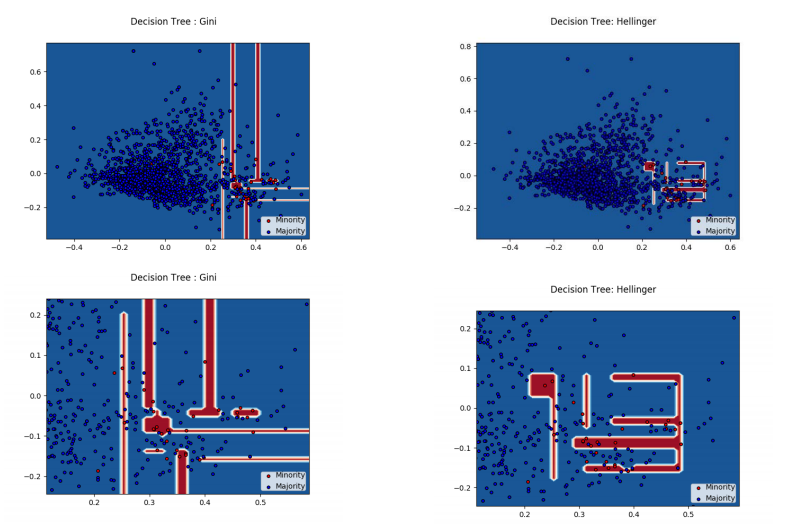
\includegraphics[width=100mm]{imagenes/hellinger-example.png}
	\label{fig:4}
	\caption{Ejemplo comportamiento algoritmo.}
\end{figure}
\verticalspace

Otra posible solución es modificar el peso asociado a clasificar mal un elemento, dando un peso mayor a clasificar mal un elemento de la clase minoritaria que de la mayoritaria, de forma que cuando se entrena el modelo intenta minimizarse el coste. El peso asociado a cada fallo se almacena en la matriz de costes, dicha matriz puede ser calculada con diferentes heurísticas o aportada por un experto en el problema que se plantee. El la siguiente imagen se muestra un ejemplo del uso de la matriz de costes para un clasificador simple.\newline

\begin{figure}[h]
	\centering
	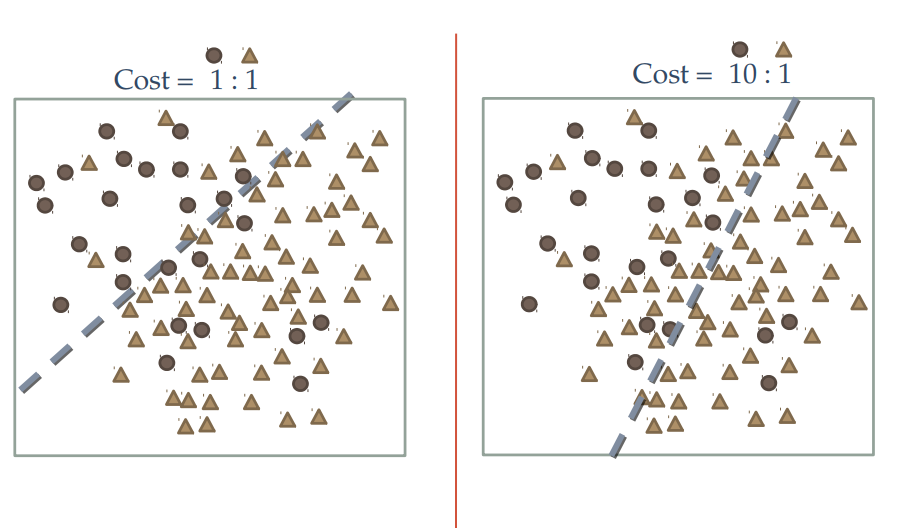
\includegraphics[width=90mm]{imagenes/cost-sentitive.png}
	\label{fig:5}
\end{figure}
\verticalspace

Existen dos formas de usar la matriz de costes, la primera es integrar el uso de la matriz dentro del algoritmo, lo que significa que hay modificarlo para que use dicha matriz; la segunda forma es preprocesando los datos de entrada asignándole un peso o asignando a cada elemento la clase que se cree que tendrá menor coste (para ello se hace uso del Teorema de Bayes).
\subsection{Técnicas basadas en la modificación del conjunto de datos}
La idea de este tipo de técnica es manipular la distribución de los datos con los que entrena el clasificador, para ello se añaden o suprimen elementos del conjunto de datos. Cuando se añaden elementos, se llama “oversampling” y cuando eliminan “undersampling”; dependiendo del problem se puede usar una de estas técnicas o ambas.\newline
\newpage
\begin{figure}[h]
	\centering
	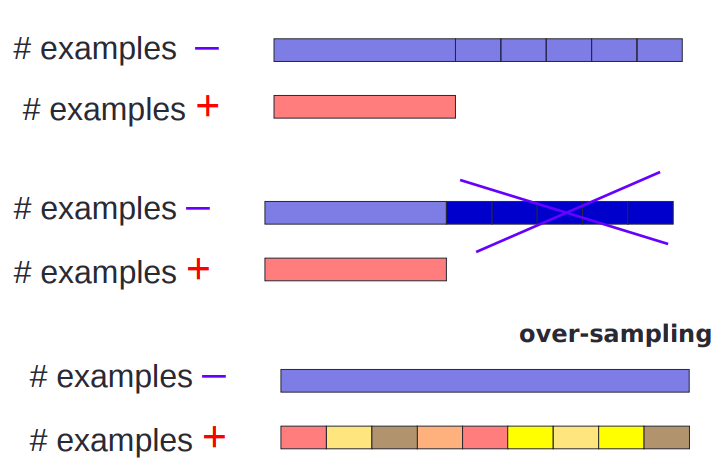
\includegraphics[width=110mm]{imagenes/oversampling_undersampling.png}
	\label{fig:6}
\end{figure}
\verticalspace

Un ejemplo clásico de algoritmo de undersampling es Tomek Links; este algoritmo elimina elementos de la clase mayoritaria que sean fronterizos con elementos de la clase minoritaria; para ello calcula las parejas de elementos de clases diferentes que estén a la distancia mínima entre ellos, es decir, que no haya ningún otro elemento dentro del conjunto de datos que su distancia hacia ese elemento sea menor; y elimina aquellos que sean de la clase mayoritaria. En la siguiente imagen se muestra un ejemplo del uso de este algoritmo.\newline


\begin{figure}[h]
	\centering
	
\includegraphics[width=120mm]{imagenes/tomek-example.png}
	\label{fig:7}
	\caption{Ejemplo funcionamiento algoritmo Tomek-Links.}
\end{figure}
\verticalspace

Otros métodos de undersampling son OSS, CNN y combinaciones de ellos. El problema del undersampling es que al eliminar elementos de la clase mayoritaria hace que cierta información se pierda, y dicha información puede ser importante al evaluar.\newline

Un algoritmo clásico de oversampling es SMOTE, este algoritmo crea nuevas instancias usando una combinación de K instancias de la clase minoritaria que sean vecinas. En la siguiente imagen se muestra un ejemplo del funcionamiento del SMOTE.\newline

\begin{figure}[h]
	\centering
	
\includegraphics[width=120mm]{imagenes/smote-example.png}
	\label{fig:8}
	\caption{Ejemplo funcionamiento algoritmo SMOTE.}
\end{figure}
\verticalspace

Otros algoritmos de oversampling son modificaciones de SMOTE, como por ejemplo Borderline-SMOTE (centrado en la generación de instancias en la frontera), ADASYN, etc.\newline

El problema del oversampling es que pueden generalizar demasiado la clase minoritaria y provocar ruido en el conjunto de datos.

\subsection{Otros enfoques}
Una última opción para paliar el desbalanceo sin implicar modificaciones de los algoritmos o del subconjunto de datos, esta es el uso de modelos ensemble; los modelos ensemble son aquellos que están formados por varios modelos más simples, para ello, los modelos simples se entrenan con un subconjunto de los datos, de forma que en esos subconjuntos el desbalanceo no tiene porque ser tan grande. Para elegir una clase, los modelos ensemble pueden combinar los resultados de los modelos simples ( para problemas de regresión ) o mediante voto. Un ejemplo de modelo ensemble es RandomForest.
\chapter{LSTMs para clasificación de series temporales}
En este capítulo se describirán el uso de las LSTM para problemas de series temporales de clasificación, así como una pequeña descripción de las LSTM y las series temporales de clasificación.
\section{Descripción}
Las LSTM son un tipo de red recurrente, esto quiere decir que tiene la capacidad de utilizar como entrada información que ya ha sido procesada; en el caso de las LSTM, dicha información es de gran importancia ya que es utilizada para calcular la salida de la LSTM a parte de la nueva información que se haya obtenido. La figura \ref{fig:31} muestra una representación de una neurona LSTM.\newline

\begin{figure}[h]
	\centering
	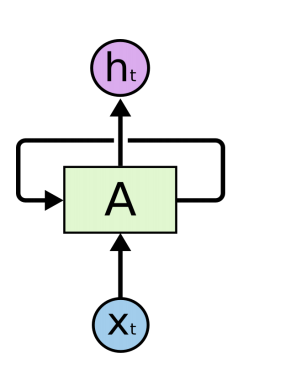
\includegraphics[width=40mm]{imagenes/lstm_basico.png}
	\caption{Ejemplo neurona LSTM.}
	\label{fig:31}
\end{figure}
\verticalspace

Las series temporales de clasificación son un caso especial de serie temporal, ya que el objetivo tras estas series no es obtener una predicción sobre el comportamiento futuro de la serie sino predecir una clase. Sobre este tipo de series temporales se pueden distinguir dos tipos: aquellos donde la serie entera corresponde con una clase y otros donde cada instante de la serie corresponde con una clase. El primer caso se podría expresar de la siguiente forma $ S \rightarrow Y $ donde $S$  es una serie cualquiera e $Y$ es la clase asociada a esta serie. El segundo caso se podría expresar de la siguiente forma $ S = (S_0, S_1,..., S_m) \rightarrow (Y_0,Y_1,..., Y_n) $ donde $S$ es una serie temporal de clasificación de longitud $n$, $S_i$ representa la serie en un momento determinado e $Y_i$ la clase asociada a dicho momento.\newline

\section{Arquitectura}
Para procesar series temporales de clasificación con LSTM se debe utilizar una estructura como la siguiente; una primera capa formadas por LSTM y una segunda capa para la predicción de la clase, esta capa no tiene por qué ser LSTM.\newline

La primera capa de esta red es la encargada de procesar la información, las LSTM procesan una serie temporal o un trozo de una serie, dependiendo del tipo de problema que se esté procesando, en cada momento; una vez procesada la información la salida de cada una de las LSTM se pasa a la segunda capa que es la encargada de predecir la clase correspondiente. Para el cálculo de la clase se utiliza una función de activación, para el caso de problemas de clasificación binaria se puede utilizar una función sigmoide, si se trata de un problema de clasificación múltiple se puede añadir tantas neuronas como clases diferentes hay o utilizar la función de activación softmax, que tiene un comportamiento muy parecido a la función sigmoide pero está adaptada a más de dos clases.\newline

Una vez se ha calcula la clase, al igual que cualquier otra red neuronal,  se comprueba si esta es correcta y se recalculan los pesos de las neuronas de la red para mejorar el rendimiento de esta; al tratarse de un problema de clasificación, las métricas de rendimiento deben ser las usuales para clasificación como por ejemplo Accuracy.\newline

La red descrita arriba es un ejemplo de la arquitectura más simple necesaria para afrontar este tipo de problemas. A partir de esta red pueden crearse redes más complejas y que en problemas específicos pueden tener un mejor rendimiento, como por ejemplo añadiendo más capas intermedias o combinando esta red con una red convolucional.\newline

Para este trabajo se utilizará la red básica descrita, ya que se utilizarán problemas diferentes para los cuales unas estructuras pueden ser más útiles que otras. La imagen \ref{fig:32} muestra un ejemplo básico de red LSTM para clasificación.

\begin{figure}[h]
	\centering
	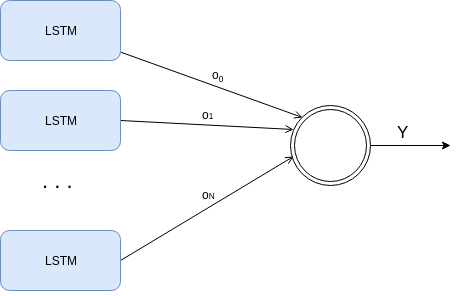
\includegraphics[width=80mm]{imagenes/arquitectura_base.png}
	\caption{Estructura básica de una red de LSTM para clasificación}
	\label{fig:32}
\end{figure}
\verticalspace

\section{Justificación}
Las series temporales son un tipo de dato que tiene dependencia temporal, es decir, el valor de una serie en un momento determinado está relacionado con el valor de la serie en momentos anteriores. Como se ha dicho al principio del capítulo, las LSTM son un tipo de red que utilizan la información anterior para procesar nueva información, por lo que lo hace adecuado para este tipo de problema.\newline

Además, las redes LSTM actualmente son un tipo de red muy utilizada en problemas complejos como la detección del habla, traducción, reconocimiento de palabras escritas a mano o incluso son utilizadas para la creación de IA capaces de jugar a videojuegos mejor que una persona.\newline

A parte de las LSTM, existen otro tipo de neuronas recurrentes como son el caso de las RNN; fueron la primera estructura recurrente para redes neuronales, tienen el inconveniente de no ser capaces de recordar información durante mucho tiempo; o las GRU, son también un tipo de neurona muy utilizada, más sencilla que las LSTM ya que tiene un número de puertas lógicas menor y más adecuada dependiendo del problema, sin embargo, al ser más sencilla no es tiene tanta potencia como las LSTM.\newline

\newpage
Por todo esto, las LSTM son una estructura válida para este trabajo y serán las que se utilicen para procesar los diferentes problemas de clasificación que se verán más adelante.\newline


\chapter{Oversampling para clasificación de series temporales}
En este capítulo se describirán diferentes algoritmos de oversampling que se utilizarán más adelante en el estudio. Con dichos algoritmos de oversampling se busca mejorar el rendimiento de los modelos que se probarán en el estudio. Los algoritmos que a continuación se van a describir son SMOTE, MWMOTE y ADASYN.

\section{SMOTE}
SMOTE (Synthetic Minority Oversampling Technique) \cite{chawla2002smote} es uno de los algoritmos de oversampling más utilizados a día de hoy. Este algortimo fue creado en 2002 y actualmente se considera como uno de los algoritmos en el estado del arte del oversampling.\newline

Para balancear los datos de las diferentes clases, SMOTE propone generar instancias de la clase minoritaria de forma sintética. Para ello, SMOTE utiliza las instancias de la clase minoritaria para generar nuevas instancias de dicha clase con características parecidas a las ya existentes.\newline

Para conseguir dicho objetivo SMOTE sigue el siguiente proceso, elige una instancia de la clase minoritaria cualquiera, tras esto se buscan sus $K$ vecinos más cercanos que sean también de la clase minoritaria; dicho parámetro $K$ se puede cambiar y afecta a como son las instancias generadas sintéticamente; si por ejemplo su valor fuera $K=1$, las instancias se generan a partir de dos instancias de la clase minoritaria, esto hace que las características de dichas instancias nuevas sean muy parecidas a las de las instancias que se han utilizado; en cambio si $K$ tiene un valor muy grande entonces las instancias generadas tienen menos parecido a las instancias con las que se han generado.\newline

Una vez se han obtenido el número de vecinos elegidos, la nueva instancia se genera como una combinación de las instancias que se utilizan, por ejemplo si $K=1$, la nueva instancia se generaría como la media de los valores de dichas instancias. El algoritmo \ref{algo:smote} muestra el pseudocodigo de este algoritmo.\newline

\begin{algorithm}[H]
	\caption{SMOTE(T,N,k)}
	\label{algo:smote}
	\begin{algorithmic}[0]
		\State \textbf{Entrada:} Número de elementos de la clase minoritaria $T$; Cantidad de instancias creadas con SMOTE $N\%$; Número de vecinos $k$
		\State \textbf{Salida:} $(N/100) * T$ instancias sintéticas de la clase minoritaria.
		\State \textit{N} = $N/100$
		\State \textit{numattrs} = número de atributos
		\State \textit{Muestra} = vector de elementos de la clase minoritaria inicial.
		\State \textit{instancias\_generadas} = guarda el número de instancias generadas, inicialmente su valor es 0.
		\State \textit{Sinteticas} = vector de elementos para guardar instancias generadas.
		\State \textit{k\_vecinos} = vector para almacenar los $k$ vecinos más cercanos.
		\For{$i \gets 1,T$}
			\State Calcular los $k$ vecinos más cercanos a $i$ y guardar el resultado en $k\_vecinos$
			\While{$N \neq 0$}
				\State Elegir un elemento de $k\_vecinos$ de forma aleatoria y llamarlo $nn$.
				\For{$attr \gets 1,numattrs$}
					\State $dif = Muestra[nn][attr] - Muestra[i][attr]$
					\State $gap =$ Número aleatorio entre 0 y 1.
					\State $Sinteticas[instancias\_generadas][attr] = Muestra[i][attr] + gap*dif$
				\EndFor
				\State $instancias\_generadas ++$
				\State $N = N-1$
			\EndWhile
		\EndFor
	\end{algorithmic}
\end{algorithm}

La figura \ref{fig:41} muestra un ejemplo de generación de instancias con SMOTE.\newline

\begin{figure}[H]
	\centering
	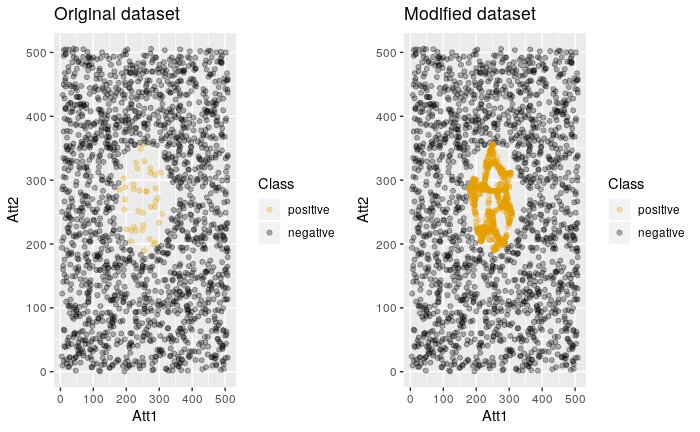
\includegraphics[width=100mm]{imagenes/SMOTE_comparison.png}
	\caption{Ejemplo de generación de instancias con SMOTE.}
	\label{fig:41}
\end{figure}
\verticalspace

Uno de los principales problemas de SMOTE es que no es bueno utilizarlo cuando las clases del conjunto de datos están mezcladas, es decir, dentro de los datos de la clase mayoritaria puede haber un pequeño conjunto de la clase minoritaria (la cual podría considerarse ruido); si se utilizara SMOTE, el número de instancias de ese conjunto sería mayor y esto afectaría al rendimiento de un modelo. Por ello, antes de utilizar este método es bueno realizar otro tipo de preprocesamientos como limpieza de ruido, imputación de valores perdidos, etc...
\newpage
\section{MWMOTE}
MWMOTE (Mayority Weighted Minority Oversampling Technique) \cite{barua2012mwmote} se trata de una modificación del algoritmo SMOTE para evitar de instancias ruidosas.\newline

El objetivo de este algoritmo es mejorar la forma de seleccionar instancias y la forma de generar las instancias sintéticas. Para ello este algoritmo cuenta con tres fases.\newline

En la primera fase se identifican los ejemplos de la clase minoritaria, a este conjunto lo podemos llamar $S_{min}$; que son más difíciles de aprender, para ello se genera un conjunto con dichos ejemplos al que llamaremos $S_{imin}$. Para generar este conjunto el algoritmo elimina todas aquellas instancias de $S_{min}$ que no tenga ninguna instancia de $S_{min}$ en su vecindario; para calcular el vecindario se utiliza el mismo proceso que para SMOTE. Una vez eliminados, se calculan aquellas instancias que son fronterizas con un conjunto de datos de la clase mayoritaria, estas instancias son las que forman $S_{imin}$.\newline

En la segunda fase, cada uno de los ejemplos de $S_{imin}$ se le agrega un peso dependiendo de la importancia de dicho ejemplo dentro de el conjunto de datos de $S_{min}$. Para ello se calcula la cantidad de información que se obtiene de cada uno de los puntos, esta medida se calcula teniendo en cuenta como de cercano está cada instancia al conjunto de datos de la clase mayoritaria. Por último, una vez calculado el peso de cada instancia se le asocia una probabilidad a dicho peso.\newline

En la tercera fase, el algoritmo genera instancias sintéticas a partir de $S_{imin}$ usando dicho peso y los añade al conjunto de datos de la clase minoritaria. Para generar dichas instancias, se detectan diferentes clústers dentro de $S_{min}$ y se por cada instancia que se genera se elige un elemento del conjunto $S_{imin}$ $x$, se elige otra instancia $y$ de $S_{min}$ que se encuentre en el mismo clúster que $x$ y se genera una nueva instancia de la siguiente forma: $ s = x + \alpha \times (y-x)$. El pseudocódigo de este algoritmo se puede encontrar en el algoritmo \ref{algo:mwmote}.

\newpage

\begin{algorithm}[H]
	\caption{MWMOTE($S_{maj},S_{min},N$)}
	\label{algo:mwmote}
	\begin{algorithmic}[0]
		\State \textit{Entrada:} Conjunto de datos de la clase mayoritaria $S_{maj}$; Conjunto de datos de la clase minoritaria $S_{min}$; Número de instancias a generar $N$
		\State \textit{Salida:} Conjunto de datos de la clase minoritaria ampliado $_{omin}$
		\ForAll{$x_i \in S_{min} $}
			\State Calcular su conjunto de vecinos más cercano, $NN(x_i)$
		\EndFor
		\State Calcular $S_{minf}$ como el conjunto de ejemplos de la clase minoritaria que no tiene ningún vecino de la clase minoritaria en su conjunto de vecinos más cercanos. $S_{minf} = S_{min} - \{x_i \in S_{min} : NN(x_i) $ no contiene ninguna instancia de $S_{min}  \}$
		\ForAll{$x_i \in S_{minf} $}
			\State Calcular conjunto de elementos más cercanos de la clase mayoritaria, $N_{maj}(x_i)$
		\EndFor
		\State Calcular el conjunto de la clase mayoritaria que forma frontera, $S_{bmaj} = \bigcup_{x_i \in S_{minf} } N_{maj}(x_i)$
		\ForAll{$y_i \in S_{bmaj}$}
			\State Calcular el conjunto de elementos más cercanos de la clase minoritaria, $N_{min} (y_i)$
		\EndFor
		\State Calcular el conjunto informativo minoritario, $S_{imin} = \bigcup_{y_i \in S_{bmaj}} N_{min}(y_i)$
		\ForAll{$y_i \in S_{bmaj}$}
			\State Calcular la cantidad de información, $I_w(y_i,x_i)$
		\EndFor
		\ForAll{$x_i \in S_{imin}$}
			\State Calcular peso de selección, $S_w(x_i) = \sum{y_i \in S_{bmaj}} I_w(y_i,x_i)$
		\EndFor
		\ForAll{$x_i \in S_{imin}$}
			\State Convertir $S_w(x_i)$ en probabilidad, $S_p(x_i) = S_w(x_i)/\sum{z_i \in S_{imin}}$
		\EndFor
		\State Calcular $M$ clúster sobre $S_{min}$, $L_1, L_2, ..., L_M$
		\State Inicializar $_{omin} = S_{min}$
		\For{$j \gets 1, N$}
			\State Seleccionar aleatoriamente un elemento $x$ de $S_imin$ con probabilidad $S_p(x)$; $x$ es un elemento perteneciente a un clúster $k$ de los calculados anteriormente.
			\State Seleccionar otra instancia $y$ aleatoriamente del clúster $k$.
			\State Crear una nueva instancia sintética $s$ como combinación lineal de las anteriores, $s = x + \alpha \times (y-x)$, donde $\alpha$ es un número aleatorio entre 0 y 1.
			\State Añadir $s$ a $S_{omin}$
		\EndFor
	\end{algorithmic}
\end{algorithm}

La figura \ref{fig:42} muestra un ejemplo de generación de instancias con MWMOTE.\newline

\begin{figure}[H]
	\centering
	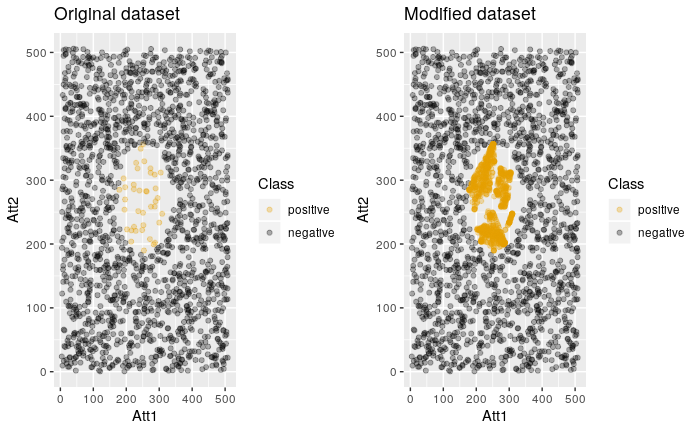
\includegraphics[width=100mm]{imagenes/MWMOTE_comparison.png}
	\caption{Ejemplo de generación de instancias con MWMOTE.}
	\label{fig:42}
\end{figure}
\verticalspace

\section{ADASYN}
ADASYN (Adaptive Synthetic Sampling) \cite{he2008adasyn} se trata de un algoritmo motivado por SMOTE. Al igual que el algoritmo de la sección anterior, propone otra forma de generar instancias. El objetivo principal de este algoritmo es reducir el sesgo entre ambas clases mientras aprende de forma adaptada. el procedimiento que sigue este algoritmo es el siguiente.\newline

Primero, calcula el ratio entre instancias de la clase minoritaria y mayoritaria; este ratio después se utiliza para calcular el número de instancias de la clase minoritaria a generar.\newline

Tras esto, por cada instancia perteneciente a la clase minoritaria, se calcula su valor $r_i$, este valor indica la dominancia de ejemplos de la clase mayoritaria en el vecindario de esta instancia; a valores mayores de esta medida es más difícil aprender sobre dicha instancia. Una vez calculadas todas las medidas se normalizan.\newline

Cuando todas las medidas $r_i$ han sido calculadas, se calcula el número de instancias a generar en el vecindario de dicha instancia de la siguiente manera: $G_i = G r_i$; donde $G$ es el número de instancias a generar que se calculó al principio.\newline
\newpage

Por último, cada una de las instancias en un vecindario $i$ se genera de la siguiente forma: se selecciona una instancia del vecindario, $x_i$; después se selecciona de forma aleatoria otra instancia vecina a la instancia $x_i$, la llamaremos $x_{zi}$; por último se calcula un número aleatorio entre 0 y 1 y se calcula la nueva instancia como la siguiente fórmula: $ s_i = x_i + (x_{zi}-x_i)\lambda$. El algoritmo \ref{algo:adasyn} muestra el pseudocodigo del algoritmo \textit{ADASYN}.

\begin{algorithm}
	\caption{ADASYN($D_{tr}, \beta, K$)}
	\label{algo:adasyn}
	\begin{algorithmic}[0]
		\State \textbf{Entrada:} Conjunto de datos de entrada $D_{tr}$; Parámetro para regular cantidad de ejemplos a crear $\beta$; Número de vecinos a tener en cuenta $K$.
		\State \textbf{Salida:} Conjunto de datos con oversampling de la clase minoritaria.
		\State $m_s$ = Número de instancias de la clase minoritaria.
		\State $m_j$ = Número de instancias de la clase mayoritaria.
		\State $d_{th}$ = Umbral máximo de desbalanceo
		\State Calcular grado de desbalanceo de clases, $d = m_s/m_j$
		\If{ $d < d_{th} $}
			\State Calcular número de instancias a generar $G = (m_j - m_s) \times \beta$
			\ForAll{$x_i \in m_s$}
				\State Calcular los $K$ vecinos más cercanos de $x_i$
				\State Calcular la dominancia de la clase positiva de $x_i$, $r_i = \bigtriangleup_i / K$, donde $\bigtriangleup_i$ es el número de vecinos de la clase positiva dentro de los $K$ vecinos de $x_i$
			\EndFor
			\State Normalizar todos los $r_i$ entre [0,1], para ello dividir cada uno sobre $\sum_{i=1}^{m_s} r_i$
			\State Calcular el número de instancias a generar por cada instancia de la clase minoritaria, $g_i = r_i \times G$
			\ForAll{$x_i \in m_s$}
				\For{$j \gets 1,g_i$}
					\State Elegir aleatoriamente un ejemplo de la clase minoritaria vecino de $x_i$, $x_{zi}$
					\State Generar una instancia sintética $s_i = x_i + (x_i - x_{zi}) \times \lambda$ donde $\lambda$ es un número aleatorio entre [0,1].
					\State Añadir $s_i$ a conjunto de datos de entrenamiento $D_{tr}$
				\EndFor
			\EndFor
		\EndIf
	\end{algorithmic}
\end{algorithm}



La figura \ref{fig:43} muestra un ejemplo de generación de instancias con ADASYN.\newline

\begin{figure}[H]
	\centering
	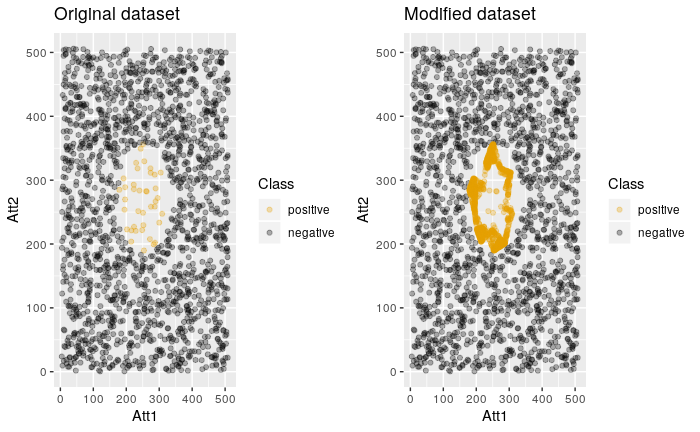
\includegraphics[width=100mm]{imagenes/ADASYN_comparison.png}
	\caption{Ejemplo de generación de instancias con ADASYN.}
	\label{fig:43}
\end{figure}
\verticalspace

Uno de los problemas de ADASYN es que puede generar instancias en vecindarios donde el número de instancias de la clase minoritaria es muy reducida, produciendo ruido.

\chapter{Tratamiento de series temporales de clasificación multivariadas}
En este capítulo se describirán las características principales de las series temporales de clasificación multivariadas, así como diferentes métodos de preprocesamiento que se han utilizado durante el estudio para limpiar dichas series he intentar mejorar los resultados.\newline

Las series temporales multivariadas de clasificación, al igual que cualquier otro conjunto de datos, deben ser preprocesadas para ofrecer un mejor rendimiento a la hora de predecir.\newline

Podemos definir una serie temporal multivariada como $S$, la cual está formada por un conjunto de series temporales univariadas, es decir $S = \{S_1,S_2,...,S_n\}$, cada una de estas series univariadas tienen sus propias características. Las series temporales multivariadas de clasificación son caso de serie temporal multivariada para las cuales además de las series univariadas existen etiquetas en el conjunto de datos. Para las series temporales multivariadas de clasificación existen dos tipos. \newline

El primer tipo de serie temporal multivariada de clasificación es aquella donde cada una de las series temporales univariadas tienen asociadas una clase, es decir $ S = \{(S_1,y_1), (S_2,y_2), ..., (S_n,y_n)\}$, donde cada $S_x$ es una serie univariada e $y_x$ es su clase asociada. Un ejemplo de serie temporal de este tipo puede ser las formadas por imágenes, cada una de las imágenes tiene una clase asociada.\newline

El segundo tipo de serie temporal multivariada es aquella donde en cada momento el conjunto de series univariadas tienen asociada un clase, es decir $S = \{(S_{11},S_{12},...,S_{1m},y_1),(S_{21},S_{22},...,S_{2m},y_2)\}, ..., (S_{n1},S_{n2},...,S_{nm},y_n) $ , donde $S_{xt}$ es el valor asociado a la serie univariada $x$ en un momento $t$ e $y_x$ es la clase asociada a dicho momento. Un ejemplo de este tipo de serie temporal puede ser predecir el movimiento de una persona a partir de los datos obtenidos de diferentes sensores.\newline

A efectos prácticos, esto significa que dependiendo del tipo de series multivariada que sea las series univariadas se encuentran como filas (primer tipo) o como columnas (segundo tipo) y se debe tener en cuenta a la hora de realizar preprocesamiento.\newline

A diferencia del tratamiento normal que se le puede hacer a  un conjunto de datos aquí se tiene que tener en cuenta que las series temporales multivariadas son un conjunto de series temporales que juntas forman la representación de un problema y hacen que sea capaz de aprender una solución. Una sola serie temporal no es suficiente para poder aprender sobre el problema que se estudie pero sí puede tener características totalmente diferentes al resto de series temporales; por ello, el preprocesamiento se debe hacer de forma individual.\newline

Un paso importante en el preprocesamiento si se están utilizando redes neuronales o cualquier otro modelo que se vea afectado por variaciones en la escala de diferentes características ( o serie temporal en este caso ) es la normalización de valores de las series.\newline

Otro tipo de tratamiento necesario para series temporales es analizar valores perdidos en la serie temporales es analizar valores perdidos en la serie. Si existen valores perdidos hay dos posibilidades; la primera es eliminar dichos valores perdidos, esta opción no es muy recomendable si la serie tiene muy pocos datos, la otra opción es imputar los valores perdidos. Para imputar dichos valores, se puede utilizar biblioteca específicas para series temporales o utilizar métodos clásicos de imputación, aunque estos no tienen por qué tener en cuenta las particularidades de las series temporales.\newline

Un buen método para imputar datos puede ser realizar un media móvil. La idea es calcular la media de los $x$ momentos anteriores y $x$ momentos siguientes, de esta forma se puede imputar cada dato con un valor cercano al resto de valores. La siguiente imagen muestra un ejemplo de media móvil. A parte de este método, se pueden utilizar métodos clásicos de predicción con series temporales como ARIMA, usando los datos anteriores al dato que se quiere imputar y realizar una predicción del valor de dicho dato con el modelo entrenado; sin embargo esto puede ser bastante costoso si hay bastantes datos perdidos ya que habría que generar un modelo para cada uno de ellos.\newline

\begin{figure}[h]
	\centering
	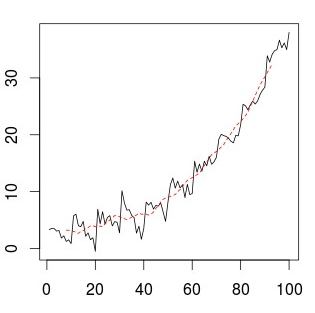
\includegraphics[width=90mm]{imagenes/moving_averages.png}
	\label{fig:11}
	\caption{Ejemplo algoritmo medias móviles.}
\end{figure}

Además de esto, también se pueden analizar los outliers que existan en la serie; si los outliers que se encuentren no aportan ninguna información adicional es mejor modificar su valor. También se podrían borrar pero esto podría provocar una pérdida de información importante, por ello es mejor no hacerlo.\newline

Para la detección de outliers se puede utilizar cualquier método de detección de outliers univariable. Un método sencillo es el cálculo de outliers mediante IQR ( InterQuartile Range, rango intercuartílico en español ), para ello se calcula el IQR, el $Q_3$ y $Q_1$ el  de los datos para los cuales se quieren detectar outliers; se consideran outliers aquellos datos que estén fuera del rango definido por $[\ Q_1 - f*IQR, Q_3+f*IQR ]\ $ , donde $f$ es una constante.\newline

Normalmente $f$ suele tomar el valor $1.5$ , pero para el caso de las series temporales este valor provoca que se detecten demasiados datos como outliers; por ello, en este estudio se ha utilizado $f=3$ para asegurarse de que los outliers detectados sean realmente anomalías en los datos de la serie y no una pequeña variación. Una vez detectados los outliers, se pueden utilizar diferentes métodos para modificar dichos outliers, por ejemplo el método comentado anteriormente ( medias móviles ).\newline

Otro proceso que se puede aplicar es crear ventanas de tiempo, es decir, en vez de utilizar solamente los datos en un momento dado, utilizar también los datos de n momentos anteriores para intentar mejorar el rendimiento de un clasificador. Elegir el tamaño de la ventana puede ser complicado ya que la ventana se aplica por igual a todas las series, por lo que requiere de experimentación para comprobar si hay una mejora en el rendimiento.\newline


\begin{figure}[h]
	\centering
	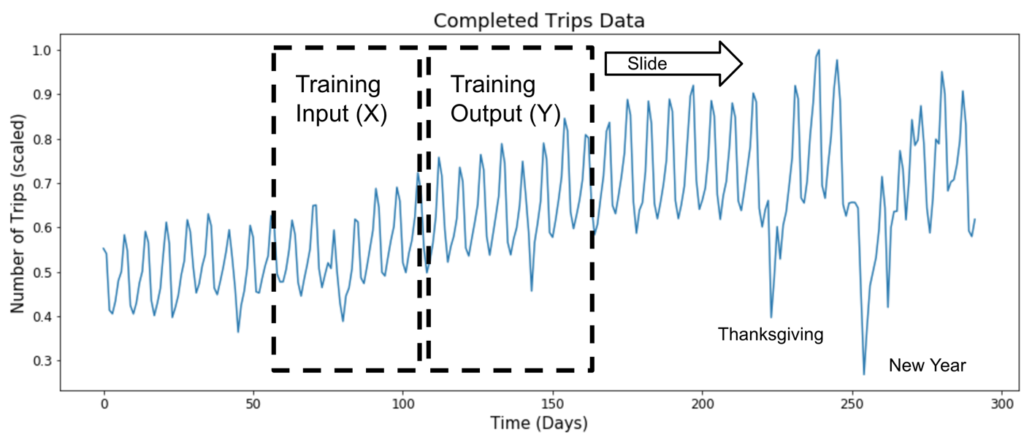
\includegraphics[width=100mm]{imagenes/sliding_window_ts.png}
	\label{fig:12}
	\caption{Ejemplo método de la ventana.}
\end{figure}
\verticalspace

Por último, se puede aplicar una selección de características, o en este caso de series temporales; para ello se pueden utilizar algoritmos de selección de características como por ejemplo Boruta, este algoritmo utiliza un modelo RandomForest y comprueba qué características son las más utilizadas 

\chapter{Marco Experimental}
En este capítulo se describirán los dataset utilizados en el estudio, además de las medidas usadas para valorar los resultados y los parámetros de la red neuronal usadas para predicción.\newline

\section{Datasets}
Los datasets utilizados para el desarrollo de este estudio son:\newline
\begin{itemize}
	\item \textbf{Adiac}. El dataset Adiac contiene los datos de un estudio sobre algas unicelulares basados en imágenes, para pasarla a series temporales se usó el contorno de cada una de las algas en las imágenes. El dataset contiene 390 instancias para entrenamiento y 391 instancias para test, cada uno de los datos cuenta con 176 características y hay 37 clases diferentes. El objetivo es aprender a diferenciar correctamente cada una de las algas.
	\item \textbf{Swedish Leaf}. El dataset Swedish Leaf se trata de un conjunto de datos que contiene el contorno de hojas de árboles suecos. Este conjunto de datos contiene 500 imágenes para entrenamiento, 625 para test, 128 características y 15 clases distintas. El objetivo es aprender a diferenciar cada una de las hojas según su silueta.
	\item \textbf{EGG eye}. La información en este dataset fue obtenida con una medición EGG (medición de actividad eléctrica en el cerebro durante un tiempo)  mediante un sensor. El objetivo de este dataset es diferenciar entre un ojo cerrado y otro abierto. El dataset contiene 14980 instancias y 15 atributos.
	\item \textbf{Face All}. El dataset contiene el contorno de 14 personas diferentes; el conjunto de entrenamiento cuenta con 560 imágenes y el conjunto de test con 1690. El objetivo es diferenciar la silueta de cada una de las personas.
	\item \textbf{Ozone}. Este dataset contiene 2536 instancias, cada una con de ellas con 73 atributos. El objetivo de este dataset es diferenciar entre un día normal y un día con niveles extraños de ozono, para ello se utilizan información de sensores sobre velocidad del viento, temperatura máxima, etc… Este conjunto de datos contiene un gran desbalanceo entre ambas clases.
	\item \textbf{HAR}. El dataset HAR contiene información sobre el movimiento de personas utilizando diferentes sensores en un móvil (giróscopo, acelerómetro, etc…). El objetivo de este dataset es diferenciar entre 6 actividades diferentes. Cada una de las instancias de este dataset contiene 561 características.
	\item \textbf{Wafer}. Este dataset contiene 2 clases, tiene 1000 datos para entrenamiento y 6164 para test; cada uno de los datos contiene 152 características. Los datos de este dataset contiene los valores de datos obtenidos por sensores (cada una de las columnas) para un proceso de creación de planchas de semiconductores para procesadores. El objetivo es distinguir entre planchas defectuosas y no defectuosas. El conjunto de datos contiene un gran desbalanceo entre clases.
	\item \textbf{Yoga}. El dataset contiene 2 clases, tiene 300 datos para entrenamiento y 3000 para test; cada uno de los datos contiene 426 características.El objetivo en este dataset es diferenciar entre una mujer y hombre realizando yoga en imágenes. Los datos que contienen este dataset transformaciones de una imagen a una señal unidimensional, para ello tomaron el outline de cada imagen y se mide la distancia de cada punto con el centro.
\end{itemize}
\verticalspace

Como se ha podido ver en la descripción, algunos de los conjuntos de datos son multiclase, por ello, dichos dataset se han transformado a problemas binarios escogiendo una clase, haciendo esa clase positiva y estableciendo el resto de clases como negativa; de esta forma también se crea desbalanceo entre clases.\newline

\section{Medidas utilizadas}
En este apartado se describirán las medidas utilizadas en el estudio, así como las características de cada una de ellas.\newline

Como ya se mencionó en el segundo capítulo, las medidas usuales no sirven para problemas con desbalanceo, por ello hay que utilizar diferentes medidas que sean útiles para este tipo de problemas.\newline

Antes de describir las diferentes medidas que se van a utilizar, se van a describir algunos conceptos básicos sobre problemas de clasificación. Un modelo de clasificación o clasificador es una función que permite decidir qué elementos de un conjunto de datos pertenecen a una cierta clase; para realizar esta decisión, el clasificador puede utilizar un umbral sobre un valor real o directamente obtener un valor discreto.\newline

Pongamos el caso de un problema de clasificación binario, en la que los datos se clasifican como positivos, lo representaremos con la letra p, o negativos, lo representaremos con la letra n. Una vez se ha entrenado un clasificador y se han obtenido los resultados, estos se pueden representar en una Matriz de confusión (para clasificación binaria es una matriz de 2x2) de la siguiente forma.\newline

\begin{figure}[h]
	\centering
	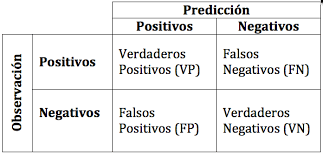
\includegraphics[width=90mm]{imagenes/conf-matrix.png}
	\label{fig:61}
	\caption{Ejemplo matriz de confusión.}
\end{figure}

Los Verdaderos Positivos (VP) son aquellos datos que han sido clasificados como positivo y su clase real es positiva, los Verdaderos Negativos (VN) son aquellos datos que han sido clasificados como negativos y su clase real es negativa, los Falsos Negativos (FN) son aquellos datos que han sido clasificados como negativos y su clase real es positiva; por último, los Falsos Positivos (FP) son aquellos datos que han sido clasificados como positivos pero su clase real es negativa.\newline

Sabiendo los valores de cada uno de estos datos, se pueden calcular medidas que contemplen un mal rendimiento por parte del clasificador al predecir alguna de las clases; esto es interesante para problemas con desbalanceo porque permite ver el rendimiento específico del clasificador para predecir la clase minoritaria.\newline

Las medidas que se utilizarán para el estudio son las siguientes: AUC, Precision, Recall, F1 Score y G-Mean.\newline

La medida Precision representa el porcentaje de los datos clasificados como positivos que realmente son positivos, es decir, de todos los datos que el clasificador ha predicho como positivos, cuántos de ellos son realmente positivos. Esta medida toma valores entre 0 y 1, valores cercanos a 1 indican un buen rendimiento por el clasificador para reconocer datos de la clase positiva. Esta medida se representa como:\newline
$$ Precision = \frac{TP}{TP + FP} $$

La medida de Recall o también conocida como True Positive Rate (TPR) representa el número el porcentaje de datos de la clase positiva que han sido clasificados como positivos. Toma valores entre 0 y 1, valores cercanos a 1 indican un buen rendimiento para reconocer la clase positiva, si el clasificador no fuera capaz de reconocer la clase positiva el número de Falsos Negativos sería muy alto y su valor se acercaría a 0.Esta medida se puede expresar como:\newline
$$ Recall = \frac{TP}{TP + FN} $$


A su vez, existe la medida True Negative Rate (TNR), que representa el porcentaje de ejemplos negativos bien clasificados, se define con la siguiente expresión.\newline
$$ TNR = \frac{TN}{TN + FP} $$

La medida F1 Score tiene en cuenta las dos anteriores para ser calculada, puede expresarse como:\newline
$$ F_1 Score = 2 * \frac{Precision*Recall}{Precision+Recall} $$

Esta medida mide el equilibrio entre las medidas Precision y Recall, si alguna de las dos tiene un valor bajo, el valor de F1 Score baja, para que aumente, el valor de ambas medidas debe aumentar. Toma valores entre 0 y 1.\newline

La medida G-Mean representa la media geométrica, sirve también para medir el equilibrio entre Precision y Recall. Se representa de la siguiente forma:\newline
$$ G-Mean = \sqrt{Precision*Recall} $$

Para esta medida, si cualquier de las medidas toma valores bajo su valor es 0.\newline
La última medida es AUC (Area Under Curve), esta medida representa el área bajo la curva ROC. La curva ROC es una representación gráfica del rendimiento entre TPR y TNR; cuanto más alto sea el valor de ambas medidas, mayor será el valor de la medida AUC.\newline

\begin{figure}[h]
	\centering
	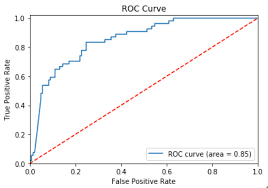
\includegraphics[width=90mm]{imagenes/auc.png}
	\label{fig:62}
	\caption{Ejemplo curva ROC.}
\end{figure}
\verticalspace

A partir de esta medida se puede medir el rendimiento de un clasificador, si el valor de AUC es 1, entonces el clasificador es perfecto. Si un clasificador hiciera las predicciones de forma aleatoria, su valor de AUC sería 0.5 y por lo tanto cualquier clasificador con valores cercanos o por debajo se considera que el clasificador es malo; para valores a partir de 0.7-0.75 se puede decir que el clasificador es aceptable.

\section{Parámetros de la red}
En este apartado se va a describir la estructura de la red utilizada en este estudio.\newline

Como se comentó anteriormente, la red usada está formada por un conjunto de LSTMs para procesar la información de las series temporales.\newline

La red básica utilizada está formada por dos capas; una capa formada por 32 LSTM y otra formada por una única neurona conectada a todas las LSTM usada para calcular la clase; para ello utiliza una función sigmoide como salida de la neurona. La estructura tendría la siguiente forma.\newline

\begin{figure}[h]
	\centering
	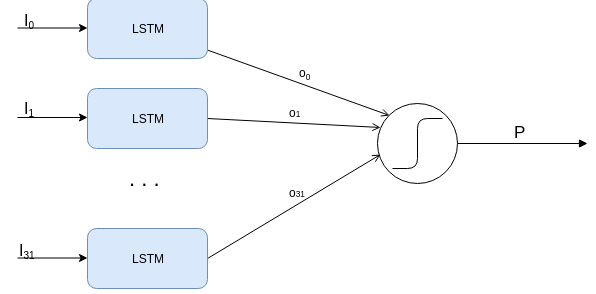
\includegraphics[width=100mm]{imagenes/Estructura_Red.png}
	\label{fig:63}
\end{figure}
\verticalspace
Cuando se define la capa de LSTM, se debe especificar el tamaño de la entrada que tendrá la LSTM; como en el caso de este estudio se utilizan diferentes tamaños de ventana, el tamaño de la entrada para la LSTM se especifica como $(1, tamventana * nseries )$, de esta forma cada LSTM procesa una ventana de información en cada momento.\newline

Por último, la red utiliza 50 epochs para entrenar y un tamaño para el batch de 16.
\chapter{Resultados y discusión}
\section{FaceAll}
\begin{table}[h]
\begin{adjustbox}{max width=16cm}
\centering
\begin{tabular}{|c|l|r|r|r|r|r|r|r|r|r|r|r|}
	\hline
	\textbf{Tam. Ventana}
	&         &      1  &      3  &      5  &      7  &      9  &      11 &      13 &      15 &      17 &      19 &      21 \\
	\hline
	\textbf{AUC} & LSTM &  0.9540 &  0.8926 &  0.8863 &  0.9315 &  0.9368 &  0.9477 &  0.9512 &  0.9432 &  0.9592 &  0.9417 &  0.9157 \\
	& SVM &  0.9423 &  0.9044 &  0.8952 &  0.8933 &  0.9216 &  0.9265 &  0.9324 &  0.9387 &  0.9276 &  0.8969 &  0.9029 \\
	& RandomForest &  0.8261 &  0.8143 &  0.8603 &  0.8182 &  0.8281 &  0.8226 &  0.8500 &  0.8276 &  0.8393 &  0.8241 &  0.8462 \\
	& XGBoost &  0.8454 &  0.8559 &  0.8673 &  0.8633 &  0.8819 &  0.9023 &  0.9000 &  0.8879 &  0.8747 &  0.8704 &  0.8365 \\
	\hline
	\textbf{F-Score} & LSTM &  0.8684 &  0.6552 &  0.4531 &  0.4549 &  0.4429 &  0.5021 &  0.4317 &  0.4628 &  0.5140 &  0.6901 &  0.5921 \\
	& SVM &  0.8951 &  0.8382 &  0.8438 &  0.8667 &  0.9076 &  0.8983 &  0.9043 &  0.9107 &  0.8972 &  0.8515 &  0.8660 \\
	& RandomForest &  0.7833 &  0.7719 &  0.8376 &  0.7778 &  0.7925 &  0.7843 &  0.8235 &  0.7917 &  0.8085 &  0.7865 &  0.8182 \\
	& XGBoost &  0.7812 &  0.8065 &  0.8403 &  0.8348 &  0.8448 &  0.8696 &  0.8889 &  0.8738 &  0.8485 &  0.8511 &  0.8046 \\
	\hline
	\textbf{G-Mean} & LSTM &  0.9533 &  0.8892 &  0.8857 &  0.9313 &  0.9362 &  0.9475 &  0.9499 &  0.9429 &  0.9590 &  0.9410 &  0.9143 \\
	& SVM &  0.9408 &  0.8999 &  0.8895 &  0.8871 &  0.9183 &  0.9237 &  0.9301 &  0.9368 &  0.9250 &  0.8913 &  0.8979 \\
	& RandomForest &  0.8077 &  0.7928 &  0.8489 &  0.7977 &  0.8101 &  0.8032 &  0.8367 &  0.8094 &  0.8238 &  0.8051 &  0.8321 \\
	& XGBoost &  0.8318 &  0.8441 &  0.8572 &  0.8525 &  0.8742 &  0.8972 &  0.8944 &  0.8808 &  0.8658 &  0.8607 &  0.8204 \\
	\hline
	\textbf{Precision} & LSTM &  0.8250 &  0.5481 &  0.3085 &  0.2986 &  0.2870 &  0.3390 &  0.2752 &  0.3043 &  0.3481 &  0.5568 &  0.4500 \\
	& SVM &  0.9014 &  0.8636 &  0.9000 &  0.9630 &  0.9818 &  0.9464 &  0.9455 &  0.9444 &  0.9412 &  0.9149 &  0.9333 \\
	& RandomForest &  0.9792 &  1.0000 &  1.0000 &  1.0000 &  1.0000 &  1.0000 &  1.0000 &  1.0000 &  1.0000 &  1.0000 &  1.0000 \\
	& XGBoost &  0.8929 &  0.9259 &  0.9804 &  0.9796 &  0.9423 &  0.9434 &  1.0000 &  1.0000 &  0.9767 &  1.0000 &  1.0000 \\
	\hline
	\textbf{Recall} & LSTM &  0.9167 &  0.8143 &  0.8529 &  0.9545 &  0.9688 &  0.9677 &  1.0000 &  0.9655 &  0.9821 &  0.9074 &  0.8654 \\
	& SVM &  0.8889 &  0.8143 &  0.7941 &  0.7879 &  0.8438 &  0.8548 &  0.8667 &  0.8793 &  0.8571 &  0.7963 &  0.8077 \\
	& RandomForest &  0.6528 &  0.6286 &  0.7206 &  0.6364 &  0.6562 &  0.6452 &  0.7000 &  0.6552 &  0.6786 &  0.6481 &  0.6923 \\
	& XGBoost &  0.6944 &  0.7143 &  0.7353 &  0.7273 &  0.7656 &  0.8065 &  0.8000 &  0.7759 &  0.7500 &  0.7407 &  0.6731 \\
	\hline
\end{tabular}
\end{adjustbox}
\label{tab:FaceAllBase}
\caption{Resultados Base FaceAll}
\end{table}
\chapter{Conclusiones y trabajos futuros}
En este capítulo se comentarán las conclusiones alcanzas después de realizar las pruebas y el análisis visto en el capítulo anterior. Tras esto, se propondrán algunas líneas de trabajo que podrían salir de este trabajo.\newline

\section{Conclusiones}
Según los resultados mostrados en el capítulo anterior, se puede afirmar que las \textit{LSTM} son un buen modelo para predicción con series temporales de clasificación, incluso si tienen desbalanceo, y competitivo con el resto de modelos de clasificación clásica.\newline

De entre los métodos de preprocesamiento utilizados, las técnicas de oversampling no han resultados ser demasiado útiles, posiblemente esto sea por el hecho de ser algoritmos generales que no están centrados en las características de las series temporales.\newline

El método de la ventana ha dado buenos resultados en la gran mayoría de casos donde el conjunto de datos era una serie temporal multivariada de clasificación con desbalanceo, o cuando la extracción de caraterísticas era la adecuada cuando se trataba de clasificación de series temporales; por lo tanto, este tipo de procesamiento es interesante utilizarlo cuando se obtienen buenos resultados de la extracción de características y cuando se trabaja con el primer tipo de serie temporal comentado.\newline

Por último, la selección de características en la mayoría de los casos ha sido la causa de obtención de modelos que clasifiquen de forma perfecta el conjunto de datos durante las pruebas, por lo que se puede concluir que la extracción de características debe ser un preprocesamiento a probar siempre y a estudiar con más profundidad para este tipo de problemas.\newline

\section{Trabajos Futuros}
Como trabajos futuros pueden realizarse las siguientes propuestas:
\begin{itemize}
	\item Desarrollo de un método de oversampling específico para series temporales que tenga en cuenta las características específicas de esta.
	\item Estudio de otras formas de combatir el desbalanceo e implementación de un optimizador de matriz de pesos con \textit{LSTMs}.
	\item Estudio del uso de la ventana en más profundidad, estudio de medidas de las redes que indiquen un cierto tamaño específico por ejemplo, algoritmo para seleccionar una ventana adecuada.
	\item Estudio de más métodos de selección de características aplicados a las series temporales de clasificación.
\end{itemize}

\nocite{*}
\addcontentsline{toc}{chapter}{Bibliografía}
\printbibliography

\chapter{Apéndice}
\appendix
\begin{table}[H]
	\begin{adjustbox}{max width=14cm}
		\centering
		\begin{tabular}{|c|l|r|r|r|r|r|r|r|r|r|r|r|}
			\hline
			\textbf{Tam. Ventana}
			&         &      1  &      3  &      5  &      7  &      9  &      11 &      13 &      15 &      17 &      19 &      21 \\
			\hline
			\textbf{AUC} & LSTM &  0.9540 &  0.8926 &  0.8863 &  0.9315 &  0.9368 &  0.9477 &  0.9512 &  0.9432 &  \textit{\textbf{0.9592}} &  0.9417 &  0.9157 \\
			& SVM &  \textbf{0.9423} &  0.9044 &  0.8952 &  0.8933 &  0.9216 &  0.9265 &  0.9324 &  0.9387 &  0.9276 &  0.8969 &  0.9029 \\
			& RandomForest &  0.8261 &  0.8143 &  \textbf{0.8603} &  0.8182 &  0.8281 &  0.8226 &  0.8500 &  0.8276 &  0.8393 &  0.8241 &  0.8462 \\
			& XGBoost &  0.8454 &  0.8559 &  0.8673 &  0.8633 &  0.8819 & \textbf{0.9023} &  0.9000 &  0.8879 &  0.8747 &  0.8704 &  0.8365 \\
			\hline
			\textbf{F-Score} & LSTM &  \textbf{0.8684} &  0.6552 &  0.4531 &  0.4549 &  0.4429 &  0.5021 &  0.4317 &  0.4628 &  0.5140 &  0.6901 &  0.5921 \\
			& SVM &  0.8951 &  0.8382 &  0.8438 &  0.8667 &  0.9076 &  0.8983 &  0.9043 &  \textit{\textbf{0.9107}} &  0.8972 &  0.8515 &  0.8660 \\
			& RandomForest &  0.7833 &  0.7719 &  \textbf{0.8376} &  0.7778 &  0.7925 &  0.7843 &  0.8235 &  0.7917 &  0.8085 &  0.7865 &  0.8182 \\
			& XGBoost &  0.7812 &  0.8065 &  0.8403 &  0.8348 &  0.8448 &  0.8696 &  \textbf{0.8889} &  0.8738 &  0.8485 &  0.8511 &  0.8046 \\
			\hline
			\textbf{G-Mean} & LSTM &  0.9533 &  0.8892 &  0.8857 &  0.9313 &  0.9362 &  0.9475 &  0.9499 &  0.9429 &  \textit{\textbf{0.9590}} &  0.9410 &  0.9143 \\
			& SVM &  \textbf{0.9408} &  0.8999 &  0.8895 &  0.8871 &  0.9183 &  0.9237 &  0.9301 &  0.9368 &  0.9250 &  0.8913 &  0.8979 \\
			& RandomForest &  0.8077 &  0.7928 &  \textbf{0.8489} &  0.7977 &  0.8101 &  0.8032 &  0.8367 &  0.8094 &  0.8238 &  0.8051 &  0.8321 \\
			& XGBoost &  0.8318 &  0.8441 &  0.8572 &  0.8525 &  0.8742 &  \textbf{0.8972} &  0.8944 &  0.8808 &  0.8658 &  0.8607 &  0.8204 \\
			\hline
			\textbf{Precision} & LSTM &  \textbf{0.8250} &  0.5481 &  0.3085 &  0.2986 &  0.2870 &  0.3390 &  0.2752 &  0.3043 &  0.3481 &  0.5568 &  0.4500 \\
			& SVM &  0.9014 &  0.8636 &  0.9000 &  0.9630 &  \textbf{0.9818} &  0.9464 &  0.9455 &  0.9444 &  0.9412 &  0.9149 &  0.9333 \\
			& RandomForest &  0.9792 &  \textit{\textbf{1.0000}} &  1.0000 &  1.0000 &  1.0000 &  1.0000 &  1.0000 &  1.0000 &  1.0000 &  1.0000 &  1.0000 \\
			& XGBoost &  0.8929 &  0.9259 &  0.9804 &  0.9796 &  0.9423 &  0.9434 &  \textbf{1.0000} &  1.0000 &  0.9767 &  1.0000 &  1.0000 \\
			\hline
			\textbf{Recall} & LSTM &  0.9167 &  0.8143 &  0.8529 &  0.9545 &  0.9688 &  0.9677 &  \textit{\textbf{1.0000}} &  0.9655 &  0.9821 &  0.9074 &  0.8654 \\
			& SVM &  \textbf{0.8889} &  0.8143 &  0.7941 &  0.7879 &  0.8438 &  0.8548 &  0.8667 &  0.8793 &  0.8571 &  0.7963 &  0.8077 \\
			& RandomForest &  0.6528 &  0.6286 &  \textbf{0.7206} &  0.6364 &  0.6562 &  0.6452 &  0.7000 &  0.6552 &  0.6786 &  0.6481 &  0.6923 \\
			& XGBoost &  0.6944 &  0.7143 &  0.7353 &  0.7273 &  0.7656 &  \textbf{0.8065} &  0.8000 &  0.7759 &  0.7500 &  0.7407 &  0.6731 \\
			\hline
		\end{tabular}
	\end{adjustbox}
	\caption{Resultados Base FaceAll.}
	\label{tab:faceAllBase}
\end{table}

\begin{table}[H]
	\centering
	\begin{adjustbox}{max width=14cm}
		\begin{tabular}{|c|l|r|r|r|r|r|r|r|r|r|r|r|}
			\hline
			\textbf{Tam. Ventana}&         &      1  &      3  &      5  &      7  &      9  &      11 &      13 &      15 &      17 &      19 &      21 \\
			\hline
			\textbf{AUC} & LSTM &  \textbf{0.9555} &  0.9228 &  0.9132 &  0.9128 &  0.9314 &  0.9255 &  0.9342 &  0.9379 &  0.9314 &  0.9083 &  0.9065 \\
			& SVM &  \textbf{0.9603} &  0.9227 &  0.9087 &  0.9303 &  0.9447 &  0.9346 &  0.9491 &  0.9473 &  0.9455 &  0.9247 &  0.9125 \\
			& RandomForest &  0.9196 &  0.8966 &  0.9173 &  0.8936 &  0.9059 &  0.9187 &  \textbf{0.9410} &  0.9221 &  0.9098 &  0.8975 &  0.9032 \\
			& XGBoost &  0.9034 &  0.9038 &  0.9092 &  0.9487 &  0.9654 &  0.9653 &  \textit{\textbf{0.9812}} &  0.9283 &  0.9141 &  0.8932 &  0.8635 \\
			\hline
			\textbf{F-Score} & LSTM &  \textbf{0.7010} &  0.6294 &  0.4300 &  0.3526 &  0.3657 &  0.3397 &  0.3604 &  0.3659 &  0.3618 &  0.3559 &  0.4299 \\
			& SVM &  0.8645 &  0.8054 &  0.8358 &  0.8906 &  \textit{\textbf{0.9268}} &  0.9076 &  0.9231 &  0.9204 &  0.9174 &  0.8846 &  0.8776 \\
			& RandomForest &  0.8356 &  0.8175 &  0.8702 &  0.8739 &  0.8889 &  0.8966 &  \textbf{0.9217} &  0.9074 &  0.8762 &  0.8687 &  0.8750 \\
			& XGBoost &  0.6857 &  0.7160 &  0.7261 &  0.8276 &  0.8889 &  0.9062 &  \textbf{0.9280} &  0.8547 &  0.7769 &  0.7611 &  0.7917 \\
			\hline
			\textbf{G-Mean} & LSTM &  \textbf{0.9555} &  0.9220 &  0.9131 &  0.9111 &  0.9289 &  0.9225 &  0.9319 &  0.9358 &  0.9300 &  0.9081 &  0.9062 \\
			& SVM &  \textbf{0.9599} &  0.9204 &  0.9047 &  0.9279 &  0.9431 &  0.9324 &  0.9478 &  0.9460 &  0.9440 &  0.9218 &  0.9085 \\
			& RandomForest &  0.9167 &  0.8914 &  0.9139 &  0.8874 &  0.9011 &  0.9152 &  \textbf{0.9393} &  0.9189 &  0.9055 &  0.8918 &  0.8982 \\
			& XGBoost &  0.9007 &  0.9006 &  0.9065 &  0.9478 &  0.9649 &  0.9648 &  \textit{\textbf{0.9811}}&  0.9259 &  0.9110 &  0.8879 &  0.8533 \\
			\hline
			\textbf{Precision} & LSTM &  \textbf{0.5574} &  0.4882 &  0.2800 &  0.2155 &  0.2238 &  0.2046 &  0.2198 &  0.2239 &  0.2218 &  0.2203 &  0.2840 \\
			& SVM &  0.8072 &  0.7595 &  0.8485 &  0.9194 &  \textbf{0.9661} &  0.9474 &  0.9474 &  0.9455 &  0.9434 &  0.9200 &  0.9348 \\
			& RandomForest &  0.8243 &  0.8358 &  0.9048 &  \textit{\textbf{0.9811}} &  0.9811 &  0.9630 &  0.9636 &  0.9800 &  0.9388 &  0.9556 &  0.9545 \\
			& XGBoost &  0.5825 &  0.6304 &  0.6404 &  0.7595 &  0.8451 &  0.8788 &  \textbf{0.8923} &  0.8475 &  0.7231 &  0.7288 &  0.8636 \\
			\hline
			\textbf{Recall} & LSTM &  0.9444 &  0.8857 &  0.9265 &  0.9697 &  \textit{\textbf{1.0000}} &  1.0000 &  1.0000 &  1.0000 &  0.9821 &  0.9259 &  0.8846 \\
			& SVM &  \textbf{0.9306} &  0.8571 &  0.8235 &  0.8636 &  0.8906 &  0.8710 &  0.9000 &  0.8966 &  0.8929 &  0.8519 &  0.8269 \\
			& RandomForest &  \textbf{0.8472} &  0.8000 &  0.8382 &  0.7879 &  0.8125 &  0.8387 &  0.8833 &  0.8448 &  0.8214 &  0.7963 &  0.8077 \\
			& XGBoost &  0.8333 &  0.8286 &  0.8382 &  0.9091 &  0.9375 &  0.9355 &  \textbf{0.9667} &  0.8621 &  0.8393 &  0.7963 &  0.7308 \\
			\hline
		\end{tabular}
	\end{adjustbox}
	\caption{Resultados FaceAll con SMOTE.}
	\label{tab:faceAllSMOTE}
\end{table}

\begin{table}[H]
	\centering
	\begin{adjustbox}{max width=14cm}
		\begin{tabular}{|c|l|r|r|r|r|r|r|r|r|r|r|r|}
			
			\hline
			\textbf{Tam. Ventana}&         &      1  &      3  &      5  &      7  &      9  &      11 &      13 &      15 &      17 &      19 &      21 \\
			\hline
			\textbf{AUC} & LSTM &  \textbf{0.9623} &  0.8861 &  0.9032 &  0.9155 &  0.9364 &  0.9140 &  0.9438 &  0.9459 &  0.9460 &  0.9157 &  0.9157 \\
			& SVM &  \textbf{0.9603} &  0.9227 &  0.9084 &  0.9230 &  0.9450 &  0.9346 &  0.9491 &  0.9387 &  0.9363 &  0.9062 &  0.9029 \\
			& RandomForest &  0.8643 &  0.8339 &  0.8597 &  0.8712 &  0.8747 &  0.8626 &  \textbf{0.8833} &  0.8017 &  0.8393 &  0.8519 &  0.8173 \\
			& XGBoost &  0.9179 &  0.8653 &  0.8890 &  0.8884 &  0.9113 &  0.9401 &  \textit{\textbf{0.9744}} &  0.8966 &  0.9018 &  0.8889 &  0.8651 \\
			\hline
			\textbf{F-Score} & LSTM &  \textbf{0.7907} &  0.5846 &  0.5221 &  0.3830 &  0.4784 &  0.3676 &  0.3974 &  0.3986 &  0.4280 &  0.4923 &  0.5000 \\
			& SVM &  0.8645 &  0.8054 &  0.8296 &  0.8889 &  \textit{\textbf{0.9344}} &  0.9076 &  0.9231 &  0.9107 &  0.8991 &  0.8627 &  0.8660 \\
			& RandomForest &  0.7737 &  0.7642 &  0.8235 &  0.8522 &  0.8496 &  0.8333 &  \textbf{0.8679} &  0.7527 &  0.8085 &  0.8261 &  0.7765 \\
			& XGBoost &  0.7086 &  0.6386 &  0.7297 &  0.7647 &  0.8413 &  0.8594 &  \textbf{0.9580} &  0.8846 &  0.8911 &  0.8750 &  0.8352 \\
			\hline
			\textbf{G-Mean} & LSTM &  \textbf{0.9622} &  0.8832 &  0.9025 &  0.9146 &  0.9362 &  0.9132 &  0.9421 &  0.9444 &  0.9453 &  0.9153 &  0.9152 \\
			& SVM &  \textbf{0.9599} &  0.9204 &  0.9044 &  0.9200 &  0.9434 &  0.9324 &  0.9478 &  0.9368 &  0.9343 &  0.9016 &  0.8979 \\
			& RandomForest &  0.8548 &  0.8179 &  0.8483 &  0.8616 &  \textbf{0.8658} &  0.8517 &  0.8756 &  0.7768 &  0.8238 &  0.8389 &  0.7966 \\
			& XGBoost &  0.9161 &  0.8585 &  0.8839 &  0.8827 &  0.9075 &  0.9387 &  \textit{\textbf{0.9741}} &  0.8906 &  0.8964 &  0.8819 &  0.8546 \\
			\hline
			\textbf{Precision} & LSTM &  \textbf{0.6800} &  0.4560 &  0.3734 &  0.2395 &  0.3194 &  0.2278 &  0.2479 &  0.2489 &  0.2736 &  0.3404 &  0.3485 \\
			& SVM &  0.8072 &  0.7595 &  0.8358 &  0.9333 &  \textbf{0.9828} &  0.9474 &  0.9474 &  0.9444 &  0.9245 &  0.9167 &  0.9333 \\
			& RandomForest &  0.8154 &  0.8868 &  0.9608 &  \textit{\textbf{1.0000}} &  0.9796 &  0.9783 &  1.0000 &  1.0000 &  1.0000 &  1.0000 &  1.0000 \\
			& XGBoost &  0.6019 &  0.5521 &  0.6750 &  0.7429 &  0.8548 &  0.8333 &  0.9661 &  \textbf{1.0000} &  1.0000 &  1.0000 &  0.9744 \\
			\hline
			\textbf{Recall} & LSTM &  0.9444 &  0.8143 &  0.8676 &  0.9545 &  0.9531 &  0.9516 &  \textit{\textbf{1.0000}} &  1.0000 &  0.9821 &  0.8889 &  0.8846 \\
			& SVM &  \textbf{0.9306} &  0.8571 &  0.8235 &  0.8485 &  0.8906 &  0.8710 &  0.9000 &  0.8793 &  0.8750 &  0.8148 &  0.8077 \\
			& RandomForest &  0.7361 &  0.6714 &  0.7206 &  0.7424 &  0.7500 &  0.7258 &  \textbf{0.7667} &  0.6034 &  0.6786 &  0.7037 &  0.6346 \\
			& XGBoost &  0.8611 &  0.7571 &  0.7941 &  0.7879 &  0.8281 &  0.8871 &  \textbf{0.9500} &  0.7931 &  0.8036 &  0.7778 &  0.7308 \\
			\hline
		\end{tabular}
	\end{adjustbox}	
	\caption{Resultados FaceAll con ADASYN.}
	\label{tab:faceAllADASYN}
\end{table}

\begin{table}[H]
	\centering
	\begin{adjustbox}{max width=14cm}
		\begin{tabular}{|c|l|r|r|r|r|r|r|r|r|r|r|r|}
			
			\hline
			\textbf{Tam. Ventana}&         &      1  &      3  &      5  &      7  &      9  &      11 &      13 &      15 &      17 &      19 &      21 \\
			\hline
			\textbf{AUC} & LSTM &  \textbf{0.9626} &  0.9240 &  0.9200 &  0.9121 &  0.9268 &  0.9292 &  0.9379 &  0.9326 &  0.9428 &  0.9101 &  0.9114 \\
			& SVM &  \textbf{0.9591} &  0.9227 &  0.9087 &  0.9306 &  0.9444 &  0.9346 &  0.9491 &  0.9470 &  0.9455 &  0.9247 &  0.9125 \\
			& RandomForest &  0.9187 &  0.8960 &  0.8964 &  0.8785 &  0.9138 &  0.8871 &  0.9083 &  0.9135 &  \textbf{0.9190} &  0.8787 &  0.8939 \\
			& XGBoost &  0.9179 &  0.9109 &  0.9249 &  0.9423 &  0.9582 &  \textit{\textbf{0.9656}} &  0.9633 &  0.9270 &  0.9055 &  0.9117 &  0.8638 \\
			\hline
			\textbf{F-Score} & LSTM &  \textbf{0.7953} &  0.5806 &  0.4649 &  0.3706 &  0.3507 &  0.3513 &  0.3738 &  0.3473 &  0.3771 &  0.3333 &  0.4646 \\
			& SVM &  0.8428 &  0.8054 &  0.8358 &  0.8976 &  0.9194 &  0.9076 &  \textit{\textbf{0.9231}} &  0.9123 &  0.9174 &  0.8846 &  0.8776 \\
			& RandomForest &  0.8188 &  0.8058 &  0.8710 &  0.8547 &  0.8983 &  0.8727 &  \textbf{0.8991} &  0.8972 &  0.8952 &  0.8367 &  0.8723 \\
			& XGBoost &  0.7086 &  0.7239 &  0.7564 &  0.8429 &  0.8939 &  \textbf{0.9134} &  0.8819 &  0.8264 &  0.7731 &  0.7826 &  0.8000 \\
			\hline
			\textbf{G-Mean} & LSTM &  \textbf{0.9625} &  0.9237 &  0.9199 &  0.9111 &  0.9239 &  0.9265 &  0.9358 &  0.9302 &  0.9411 &  0.9095 &  0.9110 \\
			& SVM &  \textbf{0.9587} &  0.9204 &  0.9047 &  0.9282 &  0.9429 &  0.9324 &  0.9478 &  0.9457 &  0.9440 &  0.9218 &  0.9085 \\
			& RandomForest &  \textbf{0.9159} &  0.8908 &  0.8906 &  0.8701 &  0.9097 &  0.8799 &  0.9037 &  0.9094 &  0.9156 &  0.8705 &  0.8877 \\
			& XGBoost &  0.9161 &  0.9084 &  0.9231 &  0.9411 &  0.9575 &  \textit{\textbf{0.9651}} &  0.9628 &  0.9247 &  0.9016 &  0.9083 &  0.8535 \\
			\hline
			\textbf{Precision} & LSTM &  \textbf{0.6869} &  0.4286 &  0.3103 &  0.2299 &  0.2126 &  0.2131 &  0.2299 &  0.2101 &  0.2324 &  0.2024 &  0.3151 \\
			& SVM &  0.7701 &  0.7595 &  0.8485 &  0.9344 &  \textbf{0.9500} &  0.9474 &  0.9474 &  0.9286 &  0.9434 &  0.9200 &  0.9348 \\
			& RandomForest &  0.7922 &  0.8116 &  0.9643 &  0.9804 &  0.9815 &  \textit{\textbf{1.0000}} &  1.0000 &  0.9796 &  0.9592 &  0.9318 &  0.9762 \\
			& XGBoost &  0.6019 &  0.6344 &  0.6705 &  0.7973 &  0.8676 &  \textbf{0.8923} &  0.8358 &  0.7937 &  0.7302 &  0.7377 &  0.8837 \\
			\hline
			\textbf{Recall} & LSTM &  0.9444 &  0.9000 &  0.9265 &  0.9545 &  \textit{\textbf{1.0000}} &  1.0000 &  1.0000 &  1.0000 &  1.0000 &  0.9444 &  0.8846 \\
			& SVM &  \textbf{0.9306} &  0.8571 &  0.8235 &  0.8636 &  0.8906 &  0.8710 &  0.9000 &  0.8966 &  0.8929 &  0.8519 &  0.8269 \\
			& RandomForest &  \textbf{0.8472} &  0.8000 &  0.7941 &  0.7576 &  0.8281 &  0.7742 &  0.8167 &  0.8276 &  0.8393 &  0.7593 &  0.7885 \\
			& XGBoost &  0.8611 &  0.8429 &  0.8676 &  0.8939 &  0.9219 &  \textbf{0.9355} &  0.9333 &  0.8621 &  0.8214 &  0.8333 &  0.7308 \\
			\hline
		\end{tabular}
	\end{adjustbox}
	\caption{Resultados FaceAll con MWMOTE.}
	\label{tab:faceAllMWMOTE}
\end{table}

\begin{table}[H]
	\centering
	\begin{adjustbox}{max width=14cm}		
		\begin{tabular}{|c|l|r|r|r|r|r|r|r|r|r|r|r|}
			\hline
			\textbf{Tam. Ventana}&         &   1  &   3  &   5  &   7  &   9  &   11 &   13 &   15 &   17 &   19 &   21 \\
			\hline
			\textbf{AUC} & LSTM &  \textit{\textbf{1.0000}} &  1.0000 &  1.0000 &  1.0000 &  1.0000 &  1.0000 &  1.0000 &  1.0000 &  1.0000 &  1.0000 &  1.0000 \\
			& SVM &  \textbf{1.0000} &  1.0000 &  1.0000 &  1.0000 &  1.0000 &  1.0000 &  1.0000 &  1.0000 &  1.0000 &  1.0000 &  1.0000 \\
			& RandomForest &  \textbf{1.0000} &  1.0000 &  1.0000 &  1.0000 &  1.0000 &  1.0000 &  1.0000 &  1.0000 &  1.0000 &  1.0000 &  1.0000 \\
			& XGBoost &  \textbf{1.0000} &  1.0000 &  1.0000 &  1.0000 &  1.0000 &  1.0000 &  1.0000 &  1.0000 &  1.0000 &  1.0000 &  1.0000 \\
			\hline
			\textbf{F-Score} & LSTM &  \textit{\textbf{1.0000}} &  1.0000 &  1.0000 &  1.0000 &  1.0000 &  1.0000 &  1.0000 &  1.0000 &  1.0000 &  1.0000 &  1.0000 \\
			& SVM &  \textbf{1.0000} &  1.0000 &  1.0000 &  1.0000 &  1.0000 &  1.0000 &  1.0000 &  1.0000 &  1.0000 &  1.0000 &  1.0000 \\
			& RandomForest &  \textbf{1.0000} &  1.0000 &  1.0000 &  1.0000 &  1.0000 &  1.0000 &  1.0000 &  1.0000 &  1.0000 &  1.0000 &  1.0000 \\
			& XGBoost &  \textbf{1.0000} &  1.0000 &  1.0000 &  1.0000 &  1.0000 &  1.0000 &  1.0000 &  1.0000 &  1.0000 &  1.0000 &  1.0000 \\
			\hline
			\textbf{G-Mean} & LSTM &  \textit{\textbf{1.0000}} &  1.0000 &  1.0000 &  1.0000 &  1.0000 &  1.0000 &  1.0000 &  1.0000 &  1.0000 &  1.0000 &  1.0000 \\
			& SVM &  \textbf{1.0000} &  1.0000 &  1.0000 &  1.0000 &  1.0000 &  1.0000 &  1.0000 &  1.0000 &  1.0000 &  1.0000 &  1.0000 \\
			& RandomForest &  \textbf{1.0000} &  1.0000 &  1.0000 &  1.0000 &  1.0000 &  1.0000 &  1.0000 &  1.0000 &  1.0000 &  1.0000 &  1.0000 \\
			& XGBoost &  \textbf{1.0000} &  1.0000 &  1.0000 &  1.0000 &  1.0000 &  1.0000 &  1.0000 &  1.0000 &  1.0000 &  1.0000 &  1.0000 \\
			\hline
			\textbf{Precision} & LSTM &  \textit{\textbf{1.0000}} &  1.0000 &  1.0000 &  1.0000 &  1.0000 &  1.0000 &  1.0000 &  1.0000 &  1.0000 &  1.0000 &  1.0000 \\
			& SVM & \textbf{1.0000} &  1.0000 &  1.0000 &  1.0000 &  1.0000 &  1.0000 &  1.0000 &  1.0000 &  1.0000 &  1.0000 &  1.0000 \\
			& RandomForest &  \textbf{1.0000} &  1.0000 &  1.0000 &  1.0000 &  1.0000 &  1.0000 &  1.0000 &  1.0000 &  1.0000 &  1.0000 &  1.0000 \\
			& XGBoost &  \textbf{1.0000} &  1.0000 &  1.0000 &  1.0000 &  1.0000 &  1.0000 &  1.0000 &  1.0000 &  1.0000 &  1.0000 &  1.0000 \\
			\hline
			\textbf{Recall} & LSTM &  \textit{\textbf{1.0000}} &  1.0000 &  1.0000 &  1.0000 &  1.0000 &  1.0000 &  1.0000 &  1.0000 &  1.0000 &  1.0000 &  1.0000 \\
			& SVM &  \textbf{1.0000} &  1.0000 &  1.0000 &  1.0000 &  1.0000 &  1.0000 &  1.0000 &  1.0000 &  1.0000 &  1.0000 &  1.0000 \\
			& RandomForest &  \textbf{1.0000} &  1.0000 &  1.0000 &  1.0000 &  1.0000 &  1.0000 &  1.0000 &  1.0000 &  1.0000 &  1.0000 &  1.0000 \\
			& XGBoost &  \textbf{1.0000} &  1.0000 &  1.0000 &  1.0000 &  1.0000 &  1.0000 &  1.0000 &  1.0000 &  1.0000 &  1.0000 &  1.0000 \\
			\hline
			
		\end{tabular}
	\end{adjustbox}
	\caption{Resultados FaceAll con SMOTE + BORUTA.}
	\label{tab:faceAllSMOTEBORUTA}
\end{table}

\begin{table}[H]
	\centering
	\begin{adjustbox}{max width=14cm}
		\begin{tabular}{|c|l|r|r|r|r|r|r|r|r|r|r|r|}
			\hline
			\textbf{Tam. Ventana}&         &   1  &   3  &   5  &   7  &   9  &   11 &   13 &   15 &   17 &   19 &   21 \\
			\hline
			\textbf{AUC} & LSTM &  \textit{\textbf{1.0000}} &  1.0000 &  1.0000 &  1.0000 &  1.0000 &  1.0000 &  1.0000 &  1.0000 &  1.0000 &  1.0000 &  1.0000 \\
			& SVM &  \textbf{1.0000} &  1.0000 &  1.0000 &  1.0000 &  1.0000 &  1.0000 &  1.0000 &  1.0000 &  1.0000 &  1.0000 &  1.0000 \\
			& RandomForest &  \textbf{1.0000} &  1.0000 &  1.0000 &  1.0000 &  1.0000 &  1.0000 &  1.0000 &  1.0000 &  1.0000 &  1.0000 &  1.0000 \\
			& XGBoost &  \textbf{1.0000} &  1.0000 &  1.0000 &  1.0000 &  1.0000 &  1.0000 &  1.0000 &  1.0000 &  1.0000 &  1.0000 &  1.0000 \\
			\hline
			\textbf{F-Score} & LSTM & \textit{ \textbf{1.0000}} &  1.0000 &  1.0000 &  1.0000 &  1.0000 &  1.0000 &  1.0000 &  1.0000 &  1.0000 &  1.0000 &  1.0000 \\
			& SVM &  \textbf{1.0000} &  1.0000 &  1.0000 &  1.0000 &  1.0000 &  1.0000 &  1.0000 &  1.0000 &  1.0000 &  1.0000 &  1.0000 \\
			& RandomForest &  \textbf{1.0000} &  1.0000 &  1.0000 &  1.0000 &  1.0000 &  1.0000 &  1.0000 &  1.0000 &  1.0000 &  1.0000 &  1.0000 \\
			& XGBoost & \textbf{ 1.0000} &  1.0000 &  1.0000 &  1.0000 &  1.0000 &  1.0000 &  1.0000 &  1.0000 &  1.0000 &  1.0000 &  1.0000 \\
			\hline
			\textbf{G-Mean} & LSTM &  \textit{\textbf{1.0000}} &  1.0000 &  1.0000 &  1.0000 &  1.0000 &  1.0000 &  1.0000 &  1.0000 &  1.0000 &  1.0000 &  1.0000 \\
			& SVM &  \textbf{1.0000} &  1.0000 &  1.0000 &  1.0000 &  1.0000 &  1.0000 &  1.0000 &  1.0000 &  1.0000 &  1.0000 &  1.0000 \\
			& RandomForest &  \textbf{1.0000} &  1.0000 &  1.0000 &  1.0000 &  1.0000 &  1.0000 &  1.0000 &  1.0000 &  1.0000 &  1.0000 &  1.0000 \\
			& XGBoost &  \textbf{1.0000} &  1.0000 &  1.0000 &  1.0000 &  1.0000 &  1.0000 &  1.0000 &  1.0000 &  1.0000 &  1.0000 &  1.0000 \\
			\hline
			\textbf{Precision} & LSTM &  \textit{\textbf{1.0000}} &  1.0000 &  1.0000 &  1.0000 &  1.0000 &  1.0000 &  1.0000 &  1.0000 &  1.0000 &  1.0000 &  1.0000 \\
			& SVM &  \textbf{1.0000} &  1.0000 &  1.0000 &  1.0000 &  1.0000 &  1.0000 &  1.0000 &  1.0000 &  1.0000 &  1.0000 &  1.0000 \\
			& RandomForest &  \textbf{1.0000} &  1.0000 &  1.0000 &  1.0000 &  1.0000 &  1.0000 &  1.0000 &  1.0000 &  1.0000 &  1.0000 &  1.0000 \\
			& XGBoost &  \textbf{1.0000} &  1.0000 &  1.0000 &  1.0000 &  1.0000 &  1.0000 &  1.0000 &  1.0000 &  1.0000 &  1.0000 &  1.0000 \\
			\hline
			\textbf{Recall} & LSTM &  \textit{\textbf{1.0000}} &  1.0000 &  1.0000 &  1.0000 &  1.0000 &  1.0000 &  1.0000 &  1.0000 &  1.0000 &  1.0000 &  1.0000 \\
			& SVM &  \textbf{1.0000} &  1.0000 &  1.0000 &  1.0000 &  1.0000 &  1.0000 &  1.0000 &  1.0000 &  1.0000 &  1.0000 &  1.0000 \\
			& RandomForest &  \textbf{1.0000} &  1.0000 &  1.0000 &  1.0000 &  1.0000 &  1.0000 &  1.0000 &  1.0000 &  1.0000 &  1.0000 &  1.0000 \\
			& XGBoost &  \textbf{1.0000} &  1.0000 &  1.0000 &  1.0000 &  1.0000 &  1.0000 &  1.0000 &  1.0000 &  1.0000 &  1.0000 &  1.0000 \\
			\hline
			
		\end{tabular}
	\end{adjustbox}	
	\caption{Resultados FaceAll con ADASYN + BORUTA.}
	\label{tab:faceAllADASYNBORUTA}
\end{table}

\begin{table}[H]
	\centering
	\begin{adjustbox}{max width=14cm}
		\begin{tabular}{|c|l|r|r|r|r|r|r|r|r|r|r|r|}
			\hline
			\textbf{Tam. Ventana}&         &   1  &   3  &   5  &   7  &   9  &   11 &   13 &   15 &   17 &   19 &   21 \\
			\hline
			\textbf{AUC} & LSTM &  \textit{\textbf{1.0000}} &  1.0000 &  1.0000 &  1.0000 &  1.0000 &  1.0000 &  1.0000 &  1.0000 &  1.0000 &  1.0000 &  1.0000 \\
			& SVM &  \textbf{1.0000} &  1.0000 &  1.0000 &  1.0000 &  1.0000 &  1.0000 &  1.0000 &  1.0000 &  1.0000 &  1.0000 &  1.0000 \\
			& RandomForest &  \textbf{1.0000} &  1.0000 &  1.0000 &  1.0000 &  1.0000 &  1.0000 &  1.0000 &  1.0000 &  1.0000 &  1.0000 &  1.0000 \\
			& XGBoost &  \textbf{1.0000} &  1.0000 &  1.0000 &  1.0000 &  1.0000 &  1.0000 &  1.0000 &  1.0000 &  1.0000 &  1.0000 &  1.0000 \\
			\hline
			\textbf{F-Score} & LSTM &  \textit{\textbf{1.0000}} &  1.0000 &  1.0000 &  1.0000 &  1.0000 &  1.0000 &  1.0000 &  1.0000 &  1.0000 &  1.0000 &  1.0000 \\
			& SVM &  \textbf{1.0000} &  1.0000 &  1.0000 &  1.0000 &  1.0000 &  1.0000 &  1.0000 &  1.0000 &  1.0000 &  1.0000 &  1.0000 \\
			& RandomForest &  \textbf{1.0000} &  1.0000 &  1.0000 &  1.0000 &  1.0000 &  1.0000 &  1.0000 &  1.0000 &  1.0000 &  1.0000 &  1.0000 \\
			& XGBoost &  \textbf{1.0000} &  1.0000 &  1.0000 &  1.0000 &  1.0000 &  1.0000 &  1.0000 &  1.0000 &  1.0000 &  1.0000 &  1.0000 \\
			\hline
			\textbf{G-Mean} & LSTM & \textit{\textbf{1.0000}} &  1.0000 &  1.0000 &  1.0000 &  1.0000 &  1.0000 &  1.0000 &  1.0000 &  1.0000 &  1.0000 &  1.0000 \\
			& SVM &  \textbf{1.0000} &  1.0000 &  1.0000 &  1.0000 &  1.0000 &  1.0000 &  1.0000 &  1.0000 &  1.0000 &  1.0000 &  1.0000 \\
			& RandomForest &  \textbf{1.0000} &  1.0000 &  1.0000 &  1.0000 &  1.0000 &  1.0000 &  1.0000 &  1.0000 &  1.0000 &  1.0000 &  1.0000 \\
			& XGBoost &  \textbf{1.0000} &  1.0000 &  1.0000 &  1.0000 &  1.0000 &  1.0000 &  1.0000 &  1.0000 &  1.0000 &  1.0000 &  1.0000 \\
			\hline
			\textbf{Precision} & LSTM &  \textit{\textbf{1.0000}} &  1.0000 &  1.0000 &  1.0000 &  1.0000 &  1.0000 &  1.0000 &  1.0000 &  1.0000 &  1.0000 &  1.0000 \\
			& SVM &  \textbf{1.0000} &  1.0000 &  1.0000 &  1.0000 &  1.0000 &  1.0000 &  1.0000 &  1.0000 &  1.0000 &  1.0000 &  1.0000 \\
			& RandomForest &  \textbf{1.0000} &  1.0000 &  1.0000 &  1.0000 &  1.0000 &  1.0000 &  1.0000 &  1.0000 &  1.0000 &  1.0000 &  1.0000 \\
			& XGBoost &  \textbf{1.0000} &  1.0000 &  1.0000 &  1.0000 &  1.0000 &  1.0000 &  1.0000 &  1.0000 &  1.0000 &  1.0000 &  1.0000 \\
			\hline
			\textbf{Recall} & LSTM &  \textit{\textbf{1.0000}} &  1.0000 &  1.0000 &  1.0000 &  1.0000 &  1.0000 &  1.0000 &  1.0000 &  1.0000 &  1.0000 &  1.0000 \\
			& SVM &  \textbf{1.0000} &  1.0000 &  1.0000 &  1.0000 &  1.0000 &  1.0000 &  1.0000 &  1.0000 &  1.0000 &  1.0000 &  1.0000 \\
			& RandomForest &  \textbf{1.0000} &  1.0000 &  1.0000 &  1.0000 &  1.0000 &  1.0000 &  1.0000 &  1.0000 &  1.0000 &  1.0000 &  1.0000 \\
			& XGBoost &  \textbf{1.0000} &  1.0000 &  1.0000 &  1.0000 &  1.0000 &  1.0000 &  1.0000 &  1.0000 &  1.0000 &  1.0000 &  1.0000 \\
			\hline
			
		\end{tabular}
	\end{adjustbox}	
	\caption{Resultados FaceAll con MWMOTE + BORUTA.}
	\label{tab:faceAllMWMOTEBORUTA}
\end{table}


\begin{table}[H]
	\centering
	\begin{adjustbox}{max width=14cm}
		\begin{tabular}{|c|l|r|r|r|r|r|r|r|r|r|r|r|}
			\hline
			\textbf{Tam. Ventana}&         &      1  &      3  &      5  &      7  &      9  &      11 &      13 &      15 &      17 &      19 &      21 \\
			\hline
			\textbf{AUC} & LSTM &  0.7666 &  0.8880 &  0.9164 &  0.9411 &  0.9485 &  0.9450 &  0.9679 &  0.9491 &  0.9693 &  0.9773 &  0.9815 \\
			& SVM &  0.6201 &  0.6315 &  0.6343 &  0.6361 &  0.6413 &  0.6503 &  0.6472 &  0.6462 &  0.6489 &  0.6646 &  0.6619 \\
			& RandomForest &  0.9282 &  0.9342 &  0.9405 &  0.9425 &  0.9496 &  0.9593 &  0.9583 &  0.9696 &  0.9658 &  0.9574 &  0.9696 \\
			& XGBoost &  0.7967 &  0.8253 &  0.8141 &  0.8253 &  0.8394 &  0.8288 &  0.8268 &  0.8466 &  0.8269 &  0.8591 &  0.8426 \\
			\hline
			\textbf{F-Score} & LSTM &  0.7275 &  0.8777 &  0.9060 &  0.9318 &  0.9447 &  0.9409 &  0.9648 &  0.9433 &  0.9637 &  0.9744 &  0.9805 \\
			& SVM &  0.4917 &  0.5100 &  0.5144 &  0.5155 &  0.5288 &  0.5483 &  0.5488 &  0.5382 &  0.5449 &  0.5774 &  0.5713 \\
			& RandomForest &  0.9196 &  0.9277 &  0.9352 &  0.9383 &  0.9457 &  0.9560 &  0.9548 &  0.9669 &  0.9635 &  0.9539 &  0.9677 \\
			& XGBoost &  0.7678 &  0.7998 &  0.7881 &  0.8014 &  0.8170 &  0.8041 &  0.8051 &  0.8272 &  0.8045 &  0.8404 &  0.8253 \\
			\hline
			\textbf{G-Mean} & LSTM &  0.7612 &  0.8878 &  0.9160 &  0.9411 &  0.9480 &  0.9439 &  0.9678 &  0.9480 &  0.9691 &  0.9773 &  0.9814 \\
			& SVM &  0.5720 &  0.5878 &  0.5903 &  0.5903 &  0.6022 &  0.6171 &  0.6164 &  0.6093 &  0.6132 &  0.6399 &  0.6341 \\
			& RandomForest &  0.9276 &  0.9339 &  0.9400 &  0.9420 &  0.9491 &  0.9591 &  0.9581 &  0.9695 &  0.9657 &  0.9573 &  0.9694 \\
			& XGBoost &  0.7934 &  0.8222 &  0.8112 &  0.8232 &  0.8376 &  0.8269 &  0.8246 &  0.8452 &  0.8251 &  0.8575 &  0.8413 \\
			\hline
			\textbf{Precision} & LSTM &  0.7881 &  0.8506 &  0.9226 &  0.9215 &  0.9720 &  0.9858 &  0.9692 &  0.8962 &  0.9386 &  0.9740 &  0.9888 \\
			& SVM &  0.6943 &  0.7016 &  0.7134 &  0.7272 &  0.7112 &  0.7138 &  0.7034 &  0.7162 &  0.7247 &  0.7135 &  0.7239 \\
			& RandomForest &  0.9436 &  0.9462 &  0.9627 &  0.9682 &  0.9746 &  0.9722 &  0.9707 &  0.9743 &  0.9773 &  0.9685 &  0.9867 \\
			& XGBoost &  0.8170 &  0.8519 &  0.8366 &  0.8388 &  0.8537 &  0.8379 &  0.8477 &  0.8576 &  0.8400 &  0.8761 &  0.8574 \\
			\hline
			\textbf{Recall} & LSTM &  0.6755 &  0.9067 &  0.8899 &  0.9423 &  0.9190 &  0.9000 &  0.9605 &  0.9956 &  0.9902 &  0.9748 &  0.9722 \\
			& SVM &  0.3807 &  0.4006 &  0.4022 &  0.3993 &  0.4209 &  0.4451 &  0.4500 &  0.4310 &  0.4365 &  0.4850 &  0.4719 \\
			& RandomForest &  0.8967 &  0.9100 &  0.9092 &  0.9103 &  0.9184 &  0.9403 &  0.9395 &  0.9597 &  0.9500 &  0.9397 &  0.9494 \\
			& XGBoost &  0.7242 &  0.7538 &  0.7449 &  0.7672 &  0.7834 &  0.7730 &  0.7667 &  0.7988 &  0.7719 &  0.8075 &  0.7956 \\
			\hline
		\end{tabular}
	\end{adjustbox}
	\caption{Resultados base EGG\_Eye.}
	\label{tab:EGGEyebase}
\end{table}
\begin{table}[H]
	\centering
	\begin{adjustbox}{max width=14cm}
		\begin{tabular}{|c|l|r|r|r|r|r|r|r|r|r|r|r|}
			\hline
			\textbf{Tam.Ventana} &         &      1  &      3  &      5  &      7  &      9  &      11 &      13 &      15 &      17 &      19 &      21 \\
			\hline
			\textbf{AUC} & LSTM &  0.5064 &  0.5433 &  0.5833 &  0.5954 &  0.5658 &  0.6151 &  0.5472 &  0.5835 &  0.5764 &  0.5581 &  0.5575 \\
			& SVM &  0.6640 &  0.6815 &  0.7013 &  0.7108 &  0.7060 &  0.7101 &  0.7139 &  0.6974 &  0.7016 &  0.7179 &  0.7150 \\
			& RandomForest &  0.9332 &  0.9389 &  0.9371 &  0.9480 &  0.9583 &  0.9538 &  0.9617 &  0.9660 &  0.9699 &  0.9710 &  0.9639 \\
			& XGBoost &  0.8069 &  0.8168 &  0.8169 &  0.8347 &  0.8491 &  0.8368 &  0.8340 &  0.8466 &  0.8471 &  0.8525 &  0.8656 \\
			\hline
			\textbf{F-Score} & LSTM &  0.6243 &  0.6367 &  0.6598 &  0.6695 &  0.6463 &  0.6805 &  0.6553 &  0.6591 &  0.6662 &  0.6415 &  0.6414 \\
			& SVM &  0.6259 &  0.6511 &  0.6697 &  0.6843 &  0.6748 &  0.6782 &  0.6853 &  0.6715 &  0.6716 &  0.6912 &  0.6844 \\
			& RandomForest &  0.9272 &  0.9345 &  0.9319 &  0.9436 &  0.9543 &  0.9499 &  0.9584 &  0.9633 &  0.9680 &  0.9691 &  0.9610 \\
			& XGBoost &  0.7866 &  0.7987 &  0.7976 &  0.8189 &  0.8316 &  0.8210 &  0.8196 &  0.8308 &  0.8354 &  0.8451 &  0.8554 \\
			\hline
			\textbf{G-Mean} & LSTM &  0.1130 &  0.2942 &  0.4088 &  0.4368 &  0.3644 &  0.4804 &  0.3074 &  0.4087 &  0.3910 &  0.3487 &  0.3391 \\
			& SVM &  0.6619 &  0.6803 &  0.7006 &  0.7100 &  0.7058 &  0.7089 &  0.7126 &  0.6972 &  0.7014 &  0.7178 &  0.7137 \\
			& RandomForest &  0.9330 &  0.9388 &  0.9364 &  0.9479 &  0.9582 &  0.9537 &  0.9617 &  0.9659 &  0.9698 &  0.9709 &  0.9638 \\
			& XGBoost &  0.8067 &  0.8166 &  0.8165 &  0.8346 &  0.8491 &  0.8363 &  0.8339 &  0.8463 &  0.8470 &  0.8525 &  0.8656 \\
			\hline
			\textbf{Precision} & LSTM &  0.4538 &  0.4670 &  0.4925 &  0.5032 &  0.4778 &  0.5159 &  0.4873 &  0.4915 &  0.4995 &  0.4736 &  0.4721 \\
			& SVM &  0.6409 &  0.6629 &  0.6684 &  0.6904 &  0.6599 &  0.6865 &  0.6998 &  0.6657 &  0.6601 &  0.6782 &  0.6962 \\
			& RandomForest &  0.9394 &  0.9434 &  0.9636 &  0.9535 &  0.9646 &  0.9633 &  0.9609 &  0.9709 &  0.9792 &  0.9811 &  0.9759 \\
			& XGBoost &  0.7834 &  0.7969 &  0.8061 &  0.8135 &  0.8248 &  0.8350 &  0.8166 &  0.8355 &  0.8351 &  0.8469 &  0.8457 \\
			\hline
			\textbf{Recall} & LSTM &  1.0000 &  1.0000 &  0.9993 &  1.0000 &  0.9985 &  0.9993 &  1.0000 &  1.0000 &  1.0000 &  0.9940 &  1.0000 \\
			& SVM &  0.6116 &  0.6398 &  0.6709 &  0.6783 &  0.6905 &  0.6701 &  0.6713 &  0.6775 &  0.6835 &  0.7046 &  0.6731 \\
			& RandomForest &  0.9152 &  0.9257 &  0.9021 &  0.9339 &  0.9443 &  0.9368 &  0.9560 &  0.9559 &  0.9571 &  0.9573 &  0.9465 \\
			& XGBoost &  0.7898 &  0.8004 &  0.7893 &  0.8243 &  0.8385 &  0.8075 &  0.8226 &  0.8262 &  0.8357 &  0.8433 &  0.8654 \\
			\hline
		\end{tabular}
	\end{adjustbox}
	\caption{Resultados base EGG\_Eye con SMOTE.}
	\label{tab:EGGEyeSMOTE}
\end{table}

\begin{table}[H]
	\centering
	\begin{adjustbox}{max width=14cm}
		\begin{tabular}{|c|l|r|r|r|r|r|r|r|r|r|r|r|}
			\hline
			\textbf{Tam. Ventana}&         &      1  &      3  &      5  &      7  &      9  &      11 &      13 &      15 &      17 &      19 &      21 \\
			\hline
			\textbf{AUC} & LSTM &  0.5047 &  0.5368 &  0.5393 &  0.5425 &  0.5511 &  0.5383 &  0.5237 &  0.5269 &  0.5411 &  0.5116 &  0.5383 \\
			& SVM &  0.6496 &  0.6801 &  0.6853 &  0.6955 &  0.7028 &  0.7078 &  0.6995 &  0.6937 &  0.7115 &  0.7075 &  0.7112 \\
			& RandomForest &  0.9299 &  0.9460 &  0.9526 &  0.9583 &  0.9660 &  0.9733 &  0.9745 &  0.9759 &  0.9694 &  0.9695 &  0.9740 \\
			& XGBoost &  0.8065 &  0.8208 &  0.8201 &  0.8338 &  0.8486 &  0.8410 &  0.8507 &  0.8487 &  0.8464 &  0.8654 &  0.8479 \\
			\hline
			\textbf{F-Score} & LSTM &  0.6094 &  0.6400 &  0.6454 &  0.6445 &  0.6433 &  0.6441 &  0.6313 &  0.6147 &  0.6453 &  0.6434 &  0.6432 \\
			& SVM &  0.6409 &  0.6556 &  0.6597 &  0.6649 &  0.6707 &  0.6700 &  0.6657 &  0.6500 &  0.6844 &  0.6790 &  0.6783 \\
			& RandomForest &  0.9217 &  0.9407 &  0.9489 &  0.9543 &  0.9623 &  0.9705 &  0.9713 &  0.9734 &  0.9667 &  0.9670 &  0.9724 \\
			& XGBoost &  0.7861 &  0.8088 &  0.8063 &  0.8203 &  0.8334 &  0.8244 &  0.8373 &  0.8328 &  0.8279 &  0.8502 &  0.8331 \\
			\hline
			\textbf{G-Mean} & LSTM &  0.0973 &  0.2714 &  0.2803 &  0.2914 &  0.3196 &  0.2768 &  0.2175 &  0.2382 &  0.2866 &  0.1525 &  0.2767 \\
			& SVM &  0.6471 &  0.6800 &  0.6853 &  0.6951 &  0.7022 &  0.7058 &  0.6987 &  0.6907 &  0.7103 &  0.7060 &  0.7080 \\
			& RandomForest &  0.9299 &  0.9460 &  0.9526 &  0.9583 &  0.9660 &  0.9733 &  0.9745 &  0.9759 &  0.9693 &  0.9695 &  0.9739 \\
			& XGBoost &  0.8061 &  0.8206 &  0.8201 &  0.8338 &  0.8486 &  0.8410 &  0.8507 &  0.8486 &  0.8464 &  0.8653 &  0.8479 \\
			\hline
			\textbf{Precision} & LSTM &  0.4383 &  0.4706 &  0.4765 &  0.4755 &  0.4742 &  0.4751 &  0.4612 &  0.4443 &  0.4764 &  0.4743 &  0.4740 \\
			& SVM &  0.5862 &  0.6404 &  0.6300 &  0.6560 &  0.6659 &  0.6856 &  0.6634 &  0.6715 &  0.6999 &  0.6979 &  0.7162 \\
			& RandomForest &  0.9220 &  0.9346 &  0.9492 &  0.9568 &  0.9663 &  0.9709 &  0.9691 &  0.9772 &  0.9729 &  0.9751 &  0.9829 \\
			& XGBoost &  0.7908 &  0.7796 &  0.7888 &  0.8138 &  0.8258 &  0.8109 &  0.8149 &  0.8148 &  0.8193 &  0.8439 &  0.8249 \\
			\hline
			\textbf{Recall} & LSTM &  1.0000 &  1.0000 &  1.0000 &  1.0000 &  1.0000 &  1.0000 &  1.0000 &  0.9969 &  1.0000 &  1.0000 &  1.0000 \\
			& SVM &  0.7068 &  0.6716 &  0.6924 &  0.6742 &  0.6755 &  0.6551 &  0.6679 &  0.6297 &  0.6696 &  0.6611 &  0.6441 \\
			& RandomForest &  0.9213 &  0.9470 &  0.9485 &  0.9518 &  0.9582 &  0.9702 &  0.9735 &  0.9698 &  0.9606 &  0.9591 &  0.9621 \\
			& XGBoost &  0.7814 &  0.8402 &  0.8247 &  0.8269 &  0.8412 &  0.8383 &  0.8610 &  0.8517 &  0.8368 &  0.8566 &  0.8415 \\
			\hline
		\end{tabular}
	\end{adjustbox}
	\caption{Resultados EGG\_Eye con ADASYN.}
	\label{tab:EGGEyeADASYN}
\end{table}
\begin{table}[H]
	\centering
	\begin{adjustbox}{max width=14cm}
		\begin{tabular}{|c|l|r|r|r|r|r|r|r|r|r|r|r|}
			\hline
			&         &      1  &      3  &      5  &      7  &      9  &      11 &      13 &      15 &      17 &      19 &      21 \\
			\hline
			\textbf{AUC} & LSTM &  0.5055 &  0.5411 &  0.5418 &  0.5724 &  0.5825 &  0.5565 &  0.5469 &  0.5439 &  0.5570 &  0.5506 &  0.5667 \\
			& SVM &  0.6911 &  0.7035 &  0.6937 &  0.6975 &  0.7044 &  0.7064 &  0.7006 &  0.7124 &  0.7046 &  0.7119 &  0.7142 \\
			& RandomForest &  0.9320 &  0.9304 &  0.9548 &  0.9546 &  0.9606 &  0.9674 &  0.9620 &  0.9648 &  0.9797 &  0.9784 &  0.9770 \\
			& XGBoost &  0.8079 &  0.8237 &  0.8284 &  0.8324 &  0.8334 &  0.8522 &  0.8398 &  0.8473 &  0.8521 &  0.8494 &  0.8739 \\
			\hline
			\textbf{F-Score} & LSTM &  0.6235 &  0.6347 &  0.6439 &  0.6558 &  0.6413 &  0.6403 &  0.6388 &  0.6550 &  0.6475 &  0.6447 &  0.6403 \\
			& SVM &  0.6726 &  0.6842 &  0.6707 &  0.6783 &  0.6811 &  0.6791 &  0.6775 &  0.6924 &  0.6758 &  0.6864 &  0.6824 \\
			& RandomForest &  0.9242 &  0.9238 &  0.9513 &  0.9499 &  0.9564 &  0.9641 &  0.9578 &  0.9618 &  0.9775 &  0.9761 &  0.9749 \\
			& XGBoost &  0.7847 &  0.8035 &  0.8128 &  0.8180 &  0.8175 &  0.8374 &  0.8211 &  0.8347 &  0.8324 &  0.8330 &  0.8665 \\
			\hline
			\textbf{G-Mean} & LSTM &  0.1045 &  0.2867 &  0.2892 &  0.3812 &  0.4062 &  0.3361 &  0.3064 &  0.2985 &  0.3375 &  0.3244 &  0.3679 \\
			& SVM &  0.6911 &  0.7034 &  0.6937 &  0.6975 &  0.7043 &  0.7064 &  0.7006 &  0.7124 &  0.7040 &  0.7118 &  0.7137 \\
			& RandomForest &  0.9320 &  0.9304 &  0.9548 &  0.9544 &  0.9605 &  0.9674 &  0.9619 &  0.9648 &  0.9797 &  0.9784 &  0.9770 \\
			& XGBoost &  0.8079 &  0.8235 &  0.8284 &  0.8324 &  0.8332 &  0.8522 &  0.8398 &  0.8473 &  0.8520 &  0.8494 &  0.8739 \\
			\hline
			\textbf{Precision} & LSTM &  0.4530 &  0.4648 &  0.4748 &  0.4880 &  0.4720 &  0.4709 &  0.4693 &  0.4874 &  0.4788 &  0.4767 &  0.4714 \\
			& SVM &  0.6609 &  0.6578 &  0.6475 &  0.6604 &  0.6705 &  0.6617 &  0.6571 &  0.6800 &  0.6753 &  0.6755 &  0.6773 \\
			& RandomForest &  0.9238 &  0.9191 &  0.9541 &  0.9598 &  0.9611 &  0.9630 &  0.9592 &  0.9664 &  0.9775 &  0.9684 &  0.9724 \\
			& XGBoost &  0.7663 &  0.7984 &  0.7971 &  0.8003 &  0.7890 &  0.8215 &  0.8000 &  0.8231 &  0.8200 &  0.8170 &  0.8601 \\
			\hline
			\textbf{Recall} & LSTM &  1.0000 &  1.0000 &  1.0000 &  0.9993 &  1.0000 &  1.0000 &  1.0000 &  0.9986 &  1.0000 &  0.9955 &  0.9977 \\
			& SVM &  0.6847 &  0.7127 &  0.6957 &  0.6971 &  0.6921 &  0.6975 &  0.6991 &  0.7053 &  0.6763 &  0.6976 &  0.6876 \\
			& RandomForest &  0.9245 &  0.9286 &  0.9486 &  0.9402 &  0.9517 &  0.9651 &  0.9564 &  0.9571 &  0.9775 &  0.9840 &  0.9774 \\
			& XGBoost &  0.8040 &  0.8086 &  0.8291 &  0.8364 &  0.8482 &  0.8540 &  0.8434 &  0.8467 &  0.8453 &  0.8497 &  0.8729 \\
			\hline
		\end{tabular}
	\end{adjustbox}
	\caption{Resultados base EGG\_Eye con MWMOTE.}
	\label{tab:EGGEyeMWMOTE}
\end{table}
\begin{table}[H]
	\centering
	\begin{adjustbox}{max width=14cm}
		\begin{tabular}{|c|l|r|r|r|r|r|r|r|r|r|r|r|}
			\hline
			\textbf{Tam. Ventana}&         &      1  &      3  &      5  &      7  &      9  &      11 &      13 &      15 &      17 &      19 &      21 \\
			\hline
			\textbf{AUC} & LSTM &  0.9566 &  0.9603 &  0.9262 &  0.9683 &  0.9513 &  0.9641 &  0.9382 &  0.9062 &  0.9459 &  0.9150 &  0.9622 \\
			& SVM &  0.9136 &  0.8876 &  0.8740 &  0.8495 &  0.8090 &  0.8109 &  0.7941 &  0.7637 &  0.7288 &  0.7557 &  0.7849 \\
			& RandomForest &  0.9512 &  0.9356 &  0.9494 &  0.9302 &  0.9262 &  0.9371 &  0.9341 &  0.9260 &  0.9545 &  0.9388 &  0.9333 \\
			& XGBoost &  0.9668 &  0.9556 &  0.9417 &  0.9543 &  0.9318 &  0.9568 &  0.9549 &  0.9408 &  0.9629 &  0.9390 &  0.9594 \\
			\hline
			\textbf{F-Score} & LSTM &  0.8814 &  0.9347 &  0.9024 &  0.9206 &  0.9239 &  0.8987 &  0.8635 &  0.8779 &  0.9223 &  0.8928 &  0.9317 \\
			& SVM &  0.8835 &  0.8394 &  0.8338 &  0.7785 &  0.7442 &  0.7420 &  0.7164 &  0.6859 &  0.6225 &  0.6645 &  0.7043 \\
			& RandomForest &  0.9238 &  0.9048 &  0.9223 &  0.9003 &  0.8939 &  0.9125 &  0.8955 &  0.8987 &  0.9216 &  0.9155 &  0.9064 \\
			& XGBoost &  0.9431 &  0.9280 &  0.9239 &  0.9242 &  0.9016 &  0.9355 &  0.9302 &  0.9010 &  0.9370 &  0.9091 &  0.9421 \\
			\hline
			\textbf{G-Mean} & LSTM &  0.9565 &  0.9598 &  0.9239 &  0.9682 &  0.9504 &  0.9641 &  0.9375 &  0.9022 &  0.9448 &  0.9117 &  0.9618 \\
			& SVM &  0.9103 &  0.8823 &  0.8662 &  0.8388 &  0.7884 &  0.7913 &  0.7700 &  0.7269 &  0.6777 &  0.7173 &  0.7575 \\
			& RandomForest &  0.9504 &  0.9341 &  0.9485 &  0.9282 &  0.9240 &  0.9355 &  0.9326 &  0.9237 &  0.9539 &  0.9373 &  0.9316 \\
			& XGBoost &  0.9665 &  0.9550 &  0.9402 &  0.9537 &  0.9300 &  0.9561 &  0.9542 &  0.9397 &  0.9625 &  0.9377 &  0.9588 \\
			\hline
			\textbf{Precision} & LSTM &  0.8273 &  0.9394 &  0.9487 &  0.8874 &  0.9362 &  0.8465 &  0.8289 &  0.9441 &  0.9453 &  0.9572 &  0.9272 \\
			& SVM &  0.9368 &  0.8950 &  0.9273 &  0.8542 &  0.9143 &  0.8951 &  0.8889 &  0.9727 &  0.9592 &  0.9273 &  0.8983 \\
			& RandomForest &  0.9353 &  0.9293 &  0.9368 &  0.9330 &  0.9267 &  0.9451 &  0.9091 &  0.9402 &  0.9216 &  0.9466 &  0.9388 \\
			& XGBoost &  0.9431 &  0.9355 &  0.9617 &  0.9289 &  0.9322 &  0.9508 &  0.9424 &  0.9055 &  0.9396 &  0.9309 &  0.9607 \\
			\hline
			\textbf{Recall} & LSTM &  0.9430 &  0.9300 &  0.8605 &  0.9563 &  0.9119 &  0.9577 &  0.9012 &  0.8204 &  0.9005 &  0.8364 &  0.9363 \\
			& SVM &  0.8359 &  0.7902 &  0.7574 &  0.7151 &  0.6275 &  0.6337 &  0.6000 &  0.5297 &  0.4608 &  0.5178 &  0.5792 \\
			& RandomForest &  0.9126 &  0.8814 &  0.9082 &  0.8698 &  0.8634 &  0.8821 &  0.8824 &  0.8607 &  0.9216 &  0.8864 &  0.8762 \\
			& XGBoost &  0.9431 &  0.9206 &  0.8889 &  0.9196 &  0.8730 &  0.9206 &  0.9184 &  0.8966 &  0.9344 &  0.8883 &  0.9243 \\
			\hline
		\end{tabular}
	\end{adjustbox}
	\caption{Resultados HAR base.}
	\label{tab:HAR_base}
\end{table}
\begin{table}[H]
	\centering
	\begin{adjustbox}{max width=14cm}
		\begin{tabular}{|c|l|r|r|r|r|r|r|r|r|r|r|r|}
			\hline
			\textbf{Tam. Ventana}&         &      1  &      3  &      5  &      7  &      9  &      11 &      13 &      15 &      17 &      19 &      21 \\
			\hline
			\textbf{AUC} & LSTM &  0.8173 &  0.8315 &  0.8459 &  0.8169 &  0.8441 &  0.8359 &  0.5000 &  0.5000 &  0.5000 &  0.5000 &  0.5000 \\
			& SVM &  0.9554 &  0.9415 &  0.9524 &  0.9429 &  0.9300 &  0.9336 &  0.9293 &  0.9208 &  0.9322 &  0.9347 &  0.9453 \\
			& RandomForest &  0.9613 &  0.9531 &  0.9581 &  0.9702 &  0.9507 &  0.9745 &  0.9449 &  0.9423 &  0.9611 &  0.9645 &  0.9541 \\
			& XGBoost &  0.9637 &  0.9576 &  0.9643 &  0.9654 &  0.9742 &  0.9591 &  0.9580 &  0.9565 &  0.9665 &  0.9663 &  0.9556 \\
			\hline
			\textbf{F-Score} & LSTM &  0.4377 &  0.4561 &  0.4855 &  0.4538 &  0.4865 &  0.4550 &  0.2313 &  0.2163 &  0.2272 &  0.2121 &  0.2261 \\
			& SVM &  0.8753 &  0.8558 &  0.8596 &  0.8414 &  0.7537 &  0.7351 &  0.7063 &  0.6904 &  0.6932 &  0.7014 &  0.7382 \\
			& RandomForest &  0.9235 &  0.9253 &  0.9227 &  0.9264 &  0.9091 &  0.9357 &  0.9110 &  0.9018 &  0.9217 &  0.9205 &  0.9152 \\
			& XGBoost &  0.9183 &  0.9066 &  0.9296 &  0.9231 &  0.9347 &  0.9096 &  0.9279 &  0.9220 &  0.9275 &  0.9364 &  0.9231 \\
			\hline
			\textbf{G-Mean} & LSTM &  0.7978 &  0.8143 &  0.8328 &  0.7961 &  0.8296 &  0.8197 &  0.0000 &  0.0000 &  0.0000 &  0.0000 &  0.0000 \\
			& SVM &  0.9553 &  0.9412 &  0.9524 &  0.9428 &  0.9300 &  0.9326 &  0.9279 &  0.9193 &  0.9304 &  0.9325 &  0.9437 \\
			& RandomForest &  0.9610 &  0.9524 &  0.9577 &  0.9701 &  0.9501 &  0.9744 &  0.9439 &  0.9413 &  0.9609 &  0.9643 &  0.9535 \\
			& XGBoost &  0.9635 &  0.9573 &  0.9640 &  0.9652 &  0.9741 &  0.9588 &  0.9575 &  0.9560 &  0.9663 &  0.9660 &  0.9551 \\
			\hline
			\textbf{Precision} & LSTM &  0.2806 &  0.2955 &  0.3211 &  0.2935 &  0.3214 &  0.2945 &  0.1308 &  0.1213 &  0.1282 &  0.1186 &  0.1275 \\
			& SVM &  0.8174 &  0.8018 &  0.7871 &  0.7671 &  0.6286 &  0.5898 &  0.5523 &  0.5344 &  0.5335 &  0.5402 &  0.5851 \\
			& RandomForest &  0.9115 &  0.9360 &  0.9158 &  0.8995 &  0.9021 &  0.9100 &  0.9206 &  0.9040 &  0.9050 &  0.8984 &  0.9082 \\
			& XGBoost &  0.8925 &  0.8824 &  0.9167 &  0.9016 &  0.9086 &  0.8844 &  0.9279 &  0.9175 &  0.9086 &  0.9293 &  0.9231 \\
			\hline
			\textbf{Recall} & LSTM &  0.9945 &  1.0000 &  0.9946 &  1.0000 &  1.0000 &  1.0000 &  1.0000 &  1.0000 &  1.0000 &  1.0000 &  1.0000 \\
			& SVM &  0.9421 &  0.9175 &  0.9469 &  0.9317 &  0.9412 &  0.9752 &  0.9794 &  0.9749 &  0.9892 &  1.0000 &  1.0000 \\
			& RandomForest &  0.9358 &  0.9148 &  0.9296 &  0.9551 &  0.9162 &  0.9630 &  0.9016 &  0.8995 &  0.9390 &  0.9438 &  0.9223 \\
			& XGBoost &  0.9455 &  0.9322 &  0.9429 &  0.9457 &  0.9624 &  0.9362 &  0.9279 &  0.9265 &  0.9471 &  0.9436 &  0.9231 \\
			\hline
		\end{tabular}
	\end{adjustbox}
	\caption{Resultados HAR con SMOTE.}
	\label{tab:HAR_SMOTE}
\end{table}

\begin{table}[H]
	\centering
	\begin{adjustbox}{max width=14cm}
		\begin{tabular}{|c|l|r|r|r|r|r|r|r|r|r|r|r|}
			\hline
			\textbf{Tam. Ventana}&         &      1  &      3  &      5  &      7  &      9  &      11 &      13 &      15 &      17 &      19 &      21 \\
			\hline
			\textbf{AUC} & LSTM &  0.8174 &  0.8349 &  0.5000 &  0.5000 &  0.5000 &  0.8418 &  0.5000 &  0.8636 &  0.8623 &  0.5000 &  0.8882 \\
			& SVM &  0.8652 &  0.8737 &  0.8931 &  0.8904 &  0.9058 &  0.9056 &  0.9126 &  0.8990 &  0.9118 &  0.9120 &  0.9170 \\
			& RandomForest &  0.9576 &  0.9440 &  0.9520 &  0.9407 &  0.9491 &  0.9500 &  0.9590 &  0.9367 &  0.9553 &  0.9593 &  0.9658 \\
			& XGBoost &  0.9582 &  0.9631 &  0.9655 &  0.9761 &  0.9405 &  0.9631 &  0.9403 &  0.9527 &  0.9590 &  0.9551 &  0.9631 \\
			\hline
			\textbf{F-Score} & LSTM &  0.4755 &  0.4809 &  0.2246 &  0.2354 &  0.2226 &  0.5019 &  0.2313 &  0.5516 &  0.5440 &  0.2272 &  0.6088 \\
			& SVM &  0.5427 &  0.5234 &  0.5924 &  0.5912 &  0.6516 &  0.6617 &  0.6475 &  0.6226 &  0.6603 &  0.6487 &  0.6688 \\
			& RandomForest &  0.9306 &  0.9038 &  0.9255 &  0.9086 &  0.9100 &  0.9091 &  0.9264 &  0.8796 &  0.9139 &  0.9077 &  0.9135 \\
			& XGBoost &  0.8790 &  0.8945 &  0.9291 &  0.9317 &  0.8951 &  0.9253 &  0.8905 &  0.9037 &  0.9023 &  0.9019 &  0.9040 \\
			\hline
			\textbf{G-Mean} & LSTM &  0.7967 &  0.8184 &  0.0000 &  0.0000 &  0.0000 &  0.8267 &  0.0000 &  0.8527 &  0.8512 &  0.0000 &  0.8818 \\
			& SVM &  0.8554 &  0.8646 &  0.8873 &  0.8836 &  0.9014 &  0.9016 &  0.9085 &  0.8949 &  0.9084 &  0.9078 &  0.9137 \\
			& RandomForest &  0.9570 &  0.9431 &  0.9513 &  0.9394 &  0.9484 &  0.9493 &  0.9586 &  0.9357 &  0.9549 &  0.9590 &  0.9657 \\
			& XGBoost &  0.9581 &  0.9630 &  0.9653 &  0.9761 &  0.9395 &  0.9628 &  0.9394 &  0.9522 &  0.9588 &  0.9548 &  0.9630 \\
			\hline
			\textbf{Precision} & LSTM &  0.3119 &  0.3166 &  0.1265 &  0.1334 &  0.1253 &  0.3350 &  0.1308 &  0.3809 &  0.3736 &  0.1282 &  0.4385 \\
			& SVM &  0.3731 &  0.3545 &  0.4217 &  0.4196 &  0.4843 &  0.4966 &  0.4788 &  0.4552 &  0.4952 &  0.4801 &  0.5037 \\
			& RandomForest &  0.9349 &  0.9038 &  0.9361 &  0.9255 &  0.9077 &  0.9043 &  0.9239 &  0.8660 &  0.9009 &  0.8792 &  0.8802 \\
			& XGBoost &  0.8203 &  0.8436 &  0.9135 &  0.8967 &  0.8929 &  0.9100 &  0.8818 &  0.8841 &  0.8661 &  0.8733 &  0.8616 \\
			\hline
			\textbf{Recall} & LSTM &  1.0000 &  1.0000 &  1.0000 &  1.0000 &  1.0000 &  1.0000 &  1.0000 &  1.0000 &  1.0000 &  1.0000 &  0.9953 \\
			& SVM &  0.9950 &  1.0000 &  0.9949 &  1.0000 &  0.9954 &  0.9910 &  1.0000 &  0.9851 &  0.9904 &  1.0000 &  0.9952 \\
			& RandomForest &  0.9263 &  0.9038 &  0.9152 &  0.8923 &  0.9124 &  0.9140 &  0.9290 &  0.8936 &  0.9272 &  0.9381 &  0.9494 \\
			& XGBoost &  0.9468 &  0.9519 &  0.9453 &  0.9695 &  0.8974 &  0.9412 &  0.8995 &  0.9242 &  0.9417 &  0.9324 &  0.9507 \\
			\hline
		\end{tabular}
	\end{adjustbox}
	\caption{Resultados HAR con ADASYN.}
	\label{tab:HAR_ADASYN}
\end{table}

\begin{table}[H]
	\centering
	\begin{adjustbox}{max width=14cm}
		\begin{tabular}{|c|l|r|r|r|r|r|r|r|r|r|r|r|}
			\hline
			\textbf{Tam. Ventana}&         &      1  &      3  &      5  &      7  &      9  &      11 &      13 &      15 &      17 &      19 &      21 \\
			\hline
			\textbf{AUC} & LSTM &  0.8216 &  0.8187 &  0.8252 &  0.5000 &  0.8431 &  0.5000 &  0.8591 &  0.5000 &  0.8857 &  0.5000 &  0.5000 \\
			& SVM &  0.8652 &  0.8737 &  0.8931 &  0.8904 &  0.9058 &  0.9056 &  0.9126 &  0.8990 &  0.9118 &  0.9120 &  0.9170 \\
			& RandomForest &  0.9740 &  0.9506 &  0.9454 &  0.9667 &  0.9536 &  0.9557 &  0.9529 &  0.9570 &  0.9524 &  0.9406 &  0.9403 \\
			& XGBoost &  0.9500 &  0.9562 &  0.9559 &  0.9538 &  0.9555 &  0.9521 &  0.9314 &  0.9462 &  0.9514 &  0.9692 &  0.9613 \\
			\hline
			\textbf{F-Score} & LSTM &  0.4977 &  0.4426 &  0.4824 &  0.2118 &  0.4833 &  0.2344 &  0.5352 &  0.2366 &  0.5706 &  0.2175 &  0.2197 \\
			& SVM &  0.5427 &  0.5234 &  0.5924 &  0.5912 &  0.6516 &  0.6617 &  0.6475 &  0.6226 &  0.6603 &  0.6487 &  0.6688 \\
			& RandomForest &  0.9457 &  0.9291 &  0.8937 &  0.9234 &  0.9263 &  0.9242 &  0.9199 &  0.9273 &  0.8976 &  0.8915 &  0.8877 \\
			& XGBoost &  0.9104 &  0.9212 &  0.9320 &  0.9039 &  0.9029 &  0.9167 &  0.8987 &  0.9081 &  0.9222 &  0.9344 &  0.9284 \\
			\hline
			\textbf{G-Mean} & LSTM &  0.8020 &  0.7983 &  0.8064 &  0.0000 &  0.8284 &  0.0000 &  0.8474 &  0.0000 &  0.8790 &  0.0000 &  0.0000 \\
			& SVM &  0.8554 &  0.8646 &  0.8873 &  0.8836 &  0.9014 &  0.9016 &  0.9085 &  0.8949 &  0.9084 &  0.9078 &  0.9137 \\
			& RandomForest &  0.9739 &  0.9497 &  0.9448 &  0.9665 &  0.9529 &  0.9552 &  0.9522 &  0.9564 &  0.9520 &  0.9398 &  0.9395 \\
			& XGBoost &  0.9494 &  0.9557 &  0.9552 &  0.9534 &  0.9552 &  0.9514 &  0.9296 &  0.9454 &  0.9506 &  0.9690 &  0.9610 \\
			\hline
			\textbf{Precision} & LSTM &  0.3313 &  0.2842 &  0.3179 &  0.1184 &  0.3186 &  0.1327 &  0.3654 &  0.1342 &  0.4000 &  0.1220 &  0.1234 \\
			& SVM &  0.3731 &  0.3545 &  0.4217 &  0.4196 &  0.4843 &  0.4966 &  0.4788 &  0.4552 &  0.4952 &  0.4801 &  0.5037 \\
			& RandomForest &  0.9337 &  0.9500 &  0.8768 &  0.8977 &  0.9362 &  0.9242 &  0.9223 &  0.9296 &  0.8724 &  0.8813 &  0.8763 \\
			& XGBoost &  0.9059 &  0.9167 &  0.9439 &  0.8832 &  0.8776 &  0.9167 &  0.9251 &  0.9105 &  0.9326 &  0.9194 &  0.9216 \\
			\hline
			\textbf{Recall} & LSTM &  1.0000 &  1.0000 &  1.0000 &  1.0000 &  1.0000 &  1.0000 &  1.0000 &  1.0000 &  0.9948 &  1.0000 &  1.0000 \\
			& SVM &  0.9950 &  1.0000 &  0.9949 &  1.0000 &  0.9954 &  0.9910 &  1.0000 &  0.9851 &  0.9904 &  1.0000 &  0.9952 \\
			& RandomForest &  0.9581 &  0.9091 &  0.9113 &  0.9507 &  0.9167 &  0.9242 &  0.9175 &  0.9250 &  0.9243 &  0.9019 &  0.8995 \\
			& XGBoost &  0.9150 &  0.9257 &  0.9204 &  0.9255 &  0.9297 &  0.9167 &  0.8737 &  0.9058 &  0.9121 &  0.9500 &  0.9353 \\
			\hline
		\end{tabular}
	\end{adjustbox}
	\caption{Resultados HAR con MWMOTE.}
	\label{tab:HAR_MWMOTE}
\end{table}

\begin{table}[H]
	\centering
	\begin{adjustbox}{max width=14cm}
		\begin{tabular}{|c|l|r|r|r|r|r|r|r|r|r|r|r|}
			\hline
			\textbf{Tam. Ventana}&         &      1  &      3  &      5  &      7  &      9  &      11 &      13 &      15 &      17 &      19 &      21 \\
			\hline
			\textbf{AUC} & LSTM &  0.8237 &  0.8395 &  0.8209 &  0.5000 &  0.8427 &  0.5000 &  0.8341 &  0.8596 &  0.5000 &  0.5000 &  0.8894 \\
			& SVM &  0.9515 &  0.9440 &  0.9491 &  0.9451 &  0.9515 &  0.9395 &  0.9435 &  0.9235 &  0.9365 &  0.9481 &  0.9404 \\
			& RandomForest &  0.9596 &  0.9684 &  0.9598 &  0.9508 &  0.9520 &  0.9580 &  0.9672 &  0.9713 &  0.9704 &  0.9575 &  0.9777 \\
			& XGBoost &  0.9659 &  0.9587 &  0.9588 &  0.9551 &  0.9533 &  0.9636 &  0.9745 &  0.9698 &  0.9568 &  0.9626 &  0.9800 \\
			\hline
			\textbf{F-Score} & LSTM &  0.4860 &  0.4804 &  0.4751 &  0.2226 &  0.4733 &  0.2291 &  0.4988 &  0.5358 &  0.2452 &  0.2357 &  0.5489 \\
			& SVM &  0.8852 &  0.8657 &  0.8556 &  0.8515 &  0.8402 &  0.7638 &  0.7083 &  0.7154 &  0.7191 &  0.7614 &  0.7251 \\
			& RandomForest &  0.9287 &  0.9293 &  0.9389 &  0.9150 &  0.9310 &  0.9254 &  0.9306 &  0.9400 &  0.9455 &  0.9197 &  0.9403 \\
			& XGBoost &  0.9208 &  0.9254 &  0.9064 &  0.8992 &  0.9105 &  0.9169 &  0.9437 &  0.9200 &  0.9188 &  0.9282 &  0.9528 \\
			\hline
			\textbf{G-Mean} & LSTM &  0.8056 &  0.8240 &  0.8012 &  0.0000 &  0.8278 &  0.0000 &  0.8175 &  0.8488 &  0.0000 &  0.0000 &  0.8825 \\
			& SVM &  0.9512 &  0.9437 &  0.9489 &  0.9450 &  0.9515 &  0.9393 &  0.9421 &  0.9230 &  0.9359 &  0.9470 &  0.9394 \\
			& RandomForest &  0.9592 &  0.9682 &  0.9593 &  0.9501 &  0.9510 &  0.9576 &  0.9670 &  0.9711 &  0.9702 &  0.9570 &  0.9777 \\
			& XGBoost &  0.9657 &  0.9583 &  0.9585 &  0.9548 &  0.9528 &  0.9634 &  0.9744 &  0.9697 &  0.9564 &  0.9623 &  0.9800 \\
			\hline
			\textbf{Precision} & LSTM &  0.3215 &  0.3161 &  0.3116 &  0.1253 &  0.3101 &  0.1293 &  0.3323 &  0.3666 &  0.1397 &  0.1336 &  0.3783 \\
			& SVM &  0.8447 &  0.8166 &  0.7913 &  0.7831 &  0.7482 &  0.6360 &  0.5502 &  0.5728 &  0.5709 &  0.6166 &  0.5742 \\
			& RandomForest &  0.9265 &  0.9096 &  0.9505 &  0.9150 &  0.9529 &  0.9231 &  0.9141 &  0.9261 &  0.9409 &  0.9121 &  0.9120 \\
			& XGBoost &  0.8942 &  0.9208 &  0.8807 &  0.8700 &  0.8990 &  0.8894 &  0.9263 &  0.8846 &  0.9083 &  0.9188 &  0.9352 \\
			\hline
			\textbf{Recall} & LSTM &  0.9952 &  1.0000 &  1.0000 &  1.0000 &  1.0000 &  1.0000 &  1.0000 &  0.9951 &  1.0000 &  1.0000 &  1.0000 \\
			& SVM &  0.9296 &  0.9212 &  0.9314 &  0.9330 &  0.9579 &  0.9558 &  0.9942 &  0.9526 &  0.9713 &  0.9950 &  0.9834 \\
			& RandomForest &  0.9310 &  0.9500 &  0.9275 &  0.9150 &  0.9101 &  0.9278 &  0.9476 &  0.9543 &  0.9502 &  0.9274 &  0.9704 \\
			& XGBoost &  0.9490 &  0.9300 &  0.9337 &  0.9305 &  0.9223 &  0.9461 &  0.9617 &  0.9583 &  0.9296 &  0.9378 &  0.9712 \\
			\hline
		\end{tabular}
	\end{adjustbox}
	\caption{Resultados HAR con SMOTE + BORUTA.}
	\label{tab:HAR_SMOTE_BORUTA}
\end{table}

\begin{table}[H]
	\centering
	\begin{adjustbox}{max width=14cm}
		\begin{tabular}{|c|l|r|r|r|r|r|r|r|r|r|r|r|}
			\hline
			&         &      1  &      3  &      5  &      7  &      9  &      11 &      13 &      15 &      17 &      19 &      21 \\
			\hline
			\textbf{AUC} & LSTM &  0.8185 &  0.8274 &  0.8214 &  0.8379 &  0.8479 &  0.8349 &  0.8414 &  0.8230 &  0.8807 &  0.5000 &  0.8502 \\
			& SVM &  0.8579 &  0.8771 &  0.8871 &  0.8882 &  0.8995 &  0.8969 &  0.9102 &  0.9207 &  0.9157 &  0.9356 &  0.9364 \\
			& RandomForest &  0.9473 &  0.9601 &  0.9571 &  0.9417 &  0.9417 &  0.9537 &  0.9566 &  0.9578 &  0.9724 &  0.9642 &  0.9629 \\
			& XGBoost &  0.9624 &  0.9588 &  0.9567 &  0.9383 &  0.9515 &  0.9494 &  0.9614 &  0.9563 &  0.9648 &  0.9600 &  0.9590 \\
			\hline
			\textbf{F-Score} & LSTM &  0.4329 &  0.4828 &  0.4909 &  0.4945 &  0.5188 &  0.5054 &  0.4762 &  0.4580 &  0.5723 &  0.2421 &  0.5116 \\
			& SVM &  0.4839 &  0.5626 &  0.5680 &  0.5684 &  0.6130 &  0.6224 &  0.6624 &  0.6805 &  0.6392 &  0.6916 &  0.7044 \\
			& RandomForest &  0.9145 &  0.9271 &  0.9311 &  0.8978 &  0.9029 &  0.9227 &  0.9282 &  0.9219 &  0.9223 &  0.9037 &  0.9319 \\
			& XGBoost &  0.8688 &  0.8998 &  0.8995 &  0.8724 &  0.8768 &  0.8954 &  0.9272 &  0.8922 &  0.9346 &  0.9187 &  0.9282 \\
			\hline
			\textbf{G-Mean} & LSTM &  0.7981 &  0.8092 &  0.8017 &  0.8221 &  0.8341 &  0.8184 &  0.8263 &  0.8038 &  0.8745 &  0.0000 &  0.8368 \\
			& SVM &  0.8460 &  0.8705 &  0.8799 &  0.8818 &  0.8944 &  0.8920 &  0.9070 &  0.9185 &  0.9123 &  0.9334 &  0.9343 \\
			& RandomForest &  0.9465 &  0.9597 &  0.9565 &  0.9408 &  0.9408 &  0.9531 &  0.9560 &  0.9573 &  0.9724 &  0.9641 &  0.9626 \\
			& XGBoost &  0.9624 &  0.9587 &  0.9566 &  0.9379 &  0.9513 &  0.9489 &  0.9611 &  0.9561 &  0.9645 &  0.9597 &  0.9585 \\
			\hline
			\textbf{Precision} & LSTM &  0.2762 &  0.3183 &  0.3253 &  0.3284 &  0.3503 &  0.3381 &  0.3125 &  0.2970 &  0.4034 &  0.1377 &  0.3437 \\
			& SVM &  0.3192 &  0.3938 &  0.3967 &  0.3978 &  0.4430 &  0.4537 &  0.4988 &  0.5198 &  0.4709 &  0.5286 &  0.5437 \\
			& RandomForest &  0.9209 &  0.9223 &  0.9378 &  0.8955 &  0.9073 &  0.9278 &  0.9330 &  0.9150 &  0.8837 &  0.8622 &  0.9271 \\
			& XGBoost &  0.7901 &  0.8596 &  0.8640 &  0.8379 &  0.8279 &  0.8720 &  0.9183 &  0.8517 &  0.9279 &  0.9014 &  0.9282 \\
			\hline
			\textbf{Recall} & LSTM &  1.0000 &  1.0000 &  1.0000 &  1.0000 &  1.0000 &  1.0000 &  1.0000 &  1.0000 &  0.9846 &  1.0000 &  1.0000 \\
			& SVM &  1.0000 &  0.9845 &  1.0000 &  0.9946 &  0.9950 &  0.9904 &  0.9857 &  0.9850 &  0.9947 &  1.0000 &  1.0000 \\
			& RandomForest &  0.9083 &  0.9319 &  0.9245 &  0.9000 &  0.8986 &  0.9176 &  0.9235 &  0.9289 &  0.9645 &  0.9494 &  0.9368 \\
			& XGBoost &  0.9648 &  0.9439 &  0.9381 &  0.9099 &  0.9319 &  0.9200 &  0.9363 &  0.9368 &  0.9415 &  0.9366 &  0.9282 \\
			\hline
		\end{tabular}
	\end{adjustbox}
	\caption{Resultados HAR con ADASYN + BORUTA.}
	\label{tab:HAR_ADASYN_BORUTA}
\end{table}

\begin{table}[H]
	\centering
	\begin{adjustbox}{max width=14cm}
		\begin{tabular}{|c|l|r|r|r|r|r|r|r|r|r|r|r|}
			\hline
			\textbf{Tam. Ventana}&         &      1  &      3  &      5  &      7  &      9  &      11 &      13 &      15 &      17 &      19 &      21 \\
			\hline
			\textbf{AUC} & LSTM &  0.8185 &  0.8274 &  0.8214 &  0.8379 &  0.8479 &  0.8349 &  0.8414 &  0.8230 &  0.8807 &  0.5000 &  0.8502 \\
			& SVM &  0.8579 &  0.8771 &  0.8871 &  0.8882 &  0.8995 &  0.8969 &  0.9102 &  0.9207 &  0.9157 &  0.9356 &  0.9364 \\
			& RandomForest &  0.9473 &  0.9601 &  0.9571 &  0.9417 &  0.9417 &  0.9537 &  0.9566 &  0.9578 &  0.9724 &  0.9642 &  0.9629 \\
			& XGBoost &  0.9624 &  0.9588 &  0.9567 &  0.9383 &  0.9515 &  0.9494 &  0.9614 &  0.9563 &  0.9648 &  0.9600 &  0.9590 \\
			\hline
			\textbf{F-Score} & LSTM &  0.4329 &  0.4828 &  0.4909 &  0.4945 &  0.5188 &  0.5054 &  0.4762 &  0.4580 &  0.5723 &  0.2421 &  0.5116 \\
			& SVM &  0.4839 &  0.5626 &  0.5680 &  0.5684 &  0.6130 &  0.6224 &  0.6624 &  0.6805 &  0.6392 &  0.6916 &  0.7044 \\
			& RandomForest &  0.9145 &  0.9271 &  0.9311 &  0.8978 &  0.9029 &  0.9227 &  0.9282 &  0.9219 &  0.9223 &  0.9037 &  0.9319 \\
			& XGBoost &  0.8688 &  0.8998 &  0.8995 &  0.8724 &  0.8768 &  0.8954 &  0.9272 &  0.8922 &  0.9346 &  0.9187 &  0.9282 \\
			\hline
			\textbf{G-Mean} & LSTM &  0.7981 &  0.8092 &  0.8017 &  0.8221 &  0.8341 &  0.8184 &  0.8263 &  0.8038 &  0.8745 &  0.0000 &  0.8368 \\
			& SVM &  0.8460 &  0.8705 &  0.8799 &  0.8818 &  0.8944 &  0.8920 &  0.9070 &  0.9185 &  0.9123 &  0.9334 &  0.9343 \\
			& RandomForest &  0.9465 &  0.9597 &  0.9565 &  0.9408 &  0.9408 &  0.9531 &  0.9560 &  0.9573 &  0.9724 &  0.9641 &  0.9626 \\
			& XGBoost &  0.9624 &  0.9587 &  0.9566 &  0.9379 &  0.9513 &  0.9489 &  0.9611 &  0.9561 &  0.9645 &  0.9597 &  0.9585 \\
			\hline
			\textbf{Precision} & LSTM &  0.2762 &  0.3183 &  0.3253 &  0.3284 &  0.3503 &  0.3381 &  0.3125 &  0.2970 &  0.4034 &  0.1377 &  0.3437 \\
			& SVM &  0.3192 &  0.3938 &  0.3967 &  0.3978 &  0.4430 &  0.4537 &  0.4988 &  0.5198 &  0.4709 &  0.5286 &  0.5437 \\
			& RandomForest &  0.9209 &  0.9223 &  0.9378 &  0.8955 &  0.9073 &  0.9278 &  0.9330 &  0.9150 &  0.8837 &  0.8622 &  0.9271 \\
			& XGBoost &  0.7901 &  0.8596 &  0.8640 &  0.8379 &  0.8279 &  0.8720 &  0.9183 &  0.8517 &  0.9279 &  0.9014 &  0.9282 \\
			\hline
			\textbf{Recall} & LSTM &  1.0000 &  1.0000 &  1.0000 &  1.0000 &  1.0000 &  1.0000 &  1.0000 &  1.0000 &  0.9846 &  1.0000 &  1.0000 \\
			& SVM &  1.0000 &  0.9845 &  1.0000 &  0.9946 &  0.9950 &  0.9904 &  0.9857 &  0.9850 &  0.9947 &  1.0000 &  1.0000 \\
			& RandomForest &  0.9083 &  0.9319 &  0.9245 &  0.9000 &  0.8986 &  0.9176 &  0.9235 &  0.9289 &  0.9645 &  0.9494 &  0.9368 \\
			& XGBoost &  0.9648 &  0.9439 &  0.9381 &  0.9099 &  0.9319 &  0.9200 &  0.9363 &  0.9368 &  0.9415 &  0.9366 &  0.9282 \\
			\hline
		\end{tabular}
	\end{adjustbox}
	\caption{Resultados HAR con MWMOTE + BORUTA.}
	\label{tab:HAR_MWMOTE_BORUTA}
\end{table}
\begin{table}[H]
	\centering
	\begin{adjustbox}{max width=14cm}
		\begin{tabular}{|c|l|r|r|r|r|r|r|r|r|r|r|r|}
			\hline
			\textbf{Tam. Ventana} &         &      1  &   3  &   5  &   7  &   9  &   11 &   13 &   15 &   17 &   19 &   21 \\
			\hline
			\textbf{AUC} & LSTM &  0.5000 &  0.5 &  0.5 &  0.5 &  0.5 &  0.5 &  0.5 &  0.5 &  0.5 &  0.5 &  0.5 \\
			& SVM &  0.5000 &  0.5 &  0.5 &  0.5 &  0.5 &  0.5 &  0.5 &  0.5 &  0.5 &  0.5 &  0.5 \\
			& RandomForest &  0.5000 &  0.5 &  0.5 &  0.5 &  0.5 &  0.5 &  0.5 &  0.5 &  0.5 &  0.5 &  0.5 \\
			& XGBoost &  0.4986 &  0.5 &  0.5 &  0.5 &  0.5 &  0.5 &  0.5 &  0.5 &  0.5 &  0.5 &  0.5 \\
			\hline
			\textbf{F-Score} & LSTM &  0.0000 &  0.0 &  0.0 &  0.0 &  0.0 &  0.0 &  0.0 &  0.0 &  0.0 &  0.0 &  0.0 \\
			& SVM &  0.0000 &  0.0 &  0.0 &  0.0 &  0.0 &  0.0 &  0.0 &  0.0 &  0.0 &  0.0 &  0.0 \\
			& RandomForest &  0.0000 &  0.0 &  0.0 &  0.0 &  0.0 &  0.0 &  0.0 &  0.0 &  0.0 &  0.0 &  0.0 \\
			& XGBoost &  0.0000 &  0.0 &  0.0 &  0.0 &  0.0 &  0.0 &  0.0 &  0.0 &  0.0 &  0.0 &  0.0 \\
			\hline
			\textbf{G-Mean} & LSTM &  0.0000 &  0.0 &  0.0 &  0.0 &  0.0 &  0.0 &  0.0 &  0.0 &  0.0 &  0.0 &  0.0 \\
			& SVM &  0.0000 &  0.0 &  0.0 &  0.0 &  0.0 &  0.0 &  0.0 &  0.0 &  0.0 &  0.0 &  0.0 \\
			& RandomForest &  0.0000 &  0.0 &  0.0 &  0.0 &  0.0 &  0.0 &  0.0 &  0.0 &  0.0 &  0.0 &  0.0 \\
			& XGBoost &  0.0000 &  0.0 &  0.0 &  0.0 &  0.0 &  0.0 &  0.0 &  0.0 &  0.0 &  0.0 &  0.0 \\
			\hline
			\textbf{Precision} & LSTM &  0.0000 &  0.0 &  0.0 &  0.0 &  0.0 &  0.0 &  0.0 &  0.0 &  0.0 &  0.0 &  0.0 \\
			& SVM &  0.0000 &  0.0 &  0.0 &  0.0 &  0.0 &  0.0 &  0.0 &  0.0 &  0.0 &  0.0 &  0.0 \\
			& RandomForest &  0.0000 &  0.0 &  0.0 &  0.0 &  0.0 &  0.0 &  0.0 &  0.0 &  0.0 &  0.0 &  0.0 \\
			& XGBoost &  0.0000 &  0.0 &  0.0 &  0.0 &  0.0 &  0.0 &  0.0 &  0.0 &  0.0 &  0.0 &  0.0 \\
			\hline
			\textbf{Recall} & LSTM &  0.0000 &  0.0 &  0.0 &  0.0 &  0.0 &  0.0 &  0.0 &  0.0 &  0.0 &  0.0 &  0.0 \\
			& SVM &  0.0000 &  0.0 &  0.0 &  0.0 &  0.0 &  0.0 &  0.0 &  0.0 &  0.0 &  0.0 &  0.0 \\
			& RandomForest &  0.0000 &  0.0 &  0.0 &  0.0 &  0.0 &  0.0 &  0.0 &  0.0 &  0.0 &  0.0 &  0.0 \\
			& XGBoost &  0.0000 &  0.0 &  0.0 &  0.0 &  0.0 &  0.0 &  0.0 &  0.0 &  0.0 &  0.0 &  0.0 \\
			\hline
		\end{tabular}
	\end{adjustbox}
	\caption{Resultados Ozone base.}
	\label{tab:Ozone_base}
\end{table}

\begin{table}[H]
	\centering
	\begin{adjustbox}{max width=14cm}
		\begin{tabular}{|c|l|r|r|r|r|r|r|r|r|r|r|r|}
			\hline
			\textbf{Tam. Ventana} &         &      1  &      3  &      5  &      7  &      9  &      11 &      13 &      15 &      17 &      19 &      21 \\
			\hline
			\textbf{AUC} & LSTM &  0.6944 &  0.7332 &  0.5000 &  0.5000 &  0.5000 &  0.5000 &  0.5000 &  0.5000 &  0.5000 &  0.5000 &  0.5000 \\
			& SVM &  0.8032 &  0.8528 &  0.8343 &  0.6475 &  0.7764 &  0.5278 &  0.7522 &  0.7373 &  0.7088 &  0.6020 &  0.6362 \\
			& RandomForest &  0.4916 &  0.4972 &  0.4986 &  0.4986 &  0.5000 &  0.5371 &  0.4986 &  0.4986 &  0.5000 &  0.5000 &  0.5000 \\
			& XGBoost &  0.5776 &  0.5554 &  0.5472 &  0.4819 &  0.5399 &  0.4807 &  0.4902 &  0.4819 &  0.5402 &  0.4902 &  0.4916 \\
			\hline
			\textbf{F-Score} & LSTM &  0.0733 &  0.1033 &  0.0476 &  0.0579 &  0.0632 &  0.0477 &  0.0633 &  0.0582 &  0.0479 &  0.0584 &  0.0584 \\
			& SVM &  0.1345 &  0.1452 &  0.1806 &  0.1364 &  0.1069 &  0.0476 &  0.0690 &  0.1566 &  0.1295 &  0.0678 &  0.1295 \\
			& RandomForest &  0.0000 &  0.0000 &  0.0000 &  0.0000 &  0.0000 &  0.1333 &  0.0000 &  0.0000 &  0.0000 &  0.0000 &  0.0000 \\
			& XGBoost &  0.1395 &  0.1600 &  0.1250 &  0.0000 &  0.1250 &  0.0000 &  0.0000 &  0.0000 &  0.0952 &  0.0000 &  0.0000 \\
			\hline
			\textbf{G-Mean} & LSTM &  0.6705 &  0.6830 &  0.0000 &  0.0000 &  0.0000 &  0.0000 &  0.0000 &  0.0000 &  0.0000 &  0.0000 &  0.0000 \\
			& SVM &  0.7986 &  0.8400 &  0.8176 &  0.6457 &  0.7701 &  0.5052 &  0.7507 &  0.7259 &  0.7076 &  0.5933 &  0.6352 \\
			& RandomForest &  0.0000 &  0.0000 &  0.0000 &  0.0000 &  0.0000 &  0.2770 &  0.0000 &  0.0000 &  0.0000 &  0.0000 &  0.0000 \\
			& XGBoost &  0.4619 &  0.3610 &  0.3305 &  0.0000 &  0.2998 &  0.0000 &  0.0000 &  0.0000 &  0.3282 &  0.0000 &  0.0000 \\
			\hline
			\textbf{Precision} & LSTM &  0.0383 &  0.0545 &  0.0244 &  0.0298 &  0.0326 &  0.0245 &  0.0327 &  0.0300 &  0.0245 &  0.0301 &  0.0301 \\
			& SVM &  0.0727 &  0.0783 &  0.0992 &  0.0769 &  0.0569 &  0.0254 &  0.0360 &  0.0861 &  0.0709 &  0.0364 &  0.0726 \\
			& RandomForest &  0.0000 &  0.0000 &  0.0000 &  0.0000 &  0.0000 &  0.5000 &  0.0000 &  0.0000 &  0.0000 &  0.0000 &  0.0000 \\
			& XGBoost &  0.1000 &  0.2000 &  0.1429 &  0.0000 &  0.2000 &  0.0000 &  0.0000 &  0.0000 &  0.0833 &  0.0000 &  0.0000 \\
			\hline
			\textbf{Recall} & LSTM &  0.8750 &  1.0000 &  1.0000 &  1.0000 &  1.0000 &  1.0000 &  1.0000 &  1.0000 &  1.0000 &  1.0000 &  1.0000 \\
			& SVM &  0.8889 &  1.0000 &  1.0000 &  0.6000 &  0.8750 &  0.3750 &  0.8000 &  0.8667 &  0.7500 &  0.5000 &  0.6000 \\
			& RandomForest &  0.0000 &  0.0000 &  0.0000 &  0.0000 &  0.0000 &  0.0769 &  0.0000 &  0.0000 &  0.0000 &  0.0000 &  0.0000 \\
			& XGBoost &  0.2308 &  0.1333 &  0.1111 &  0.0000 &  0.0909 &  0.0000 &  0.0000 &  0.0000 &  0.1111 &  0.0000 &  0.0000 \\
			\hline
		\end{tabular}
	\end{adjustbox}
	\caption{Resultados Ozone con SMOTE.}
	\label{tab:Ozone_SMOTE}
\end{table}

\begin{table}[H]
	\centering
	\begin{adjustbox}{max width=14cm}
		\begin{tabular}{|c|l|r|r|r|r|r|r|r|r|r|r|r|}
			\hline
			\textbf{Tam. Ventana} &         &      1  &      3  &      5  &      7  &      9  &      11 &      13 &      15 &      17 &      19 &      21 \\
			\hline
			\textbf{AUC} & LSTM &  0.6396 &  0.6826 &  0.5000 &  0.5000 &  0.5000 &  0.5000 &  0.5000 &  0.5000 &  0.5000 &  0.5000 &  0.5000 \\
			& SVM &  0.7949 &  0.8333 &  0.7541 &  0.7238 &  0.6093 &  0.5792 &  0.6323 &  0.7745 &  0.6948 &  0.7431 &  0.6909 \\
			& RandomForest &  0.4944 &  0.4986 &  0.4972 &  0.5000 &  0.5000 &  0.5000 &  0.5000 &  0.5000 &  0.5000 &  0.5000 &  0.5000 \\
			& XGBoost &  0.5503 &  0.5361 &  0.4819 &  0.5473 &  0.5227 &  0.5360 &  0.4872 &  0.4889 &  0.6151 &  0.5684 &  0.5430 \\
			\hline
			\textbf{F-Score} & LSTM &  0.0714 &  0.0853 &  0.0630 &  0.0630 &  0.0426 &  0.0580 &  0.0322 &  0.0735 &  0.1034 &  0.0737 &  0.0428 \\
			& SVM &  0.1571 &  0.1678 &  0.1374 &  0.1517 &  0.0741 &  0.0593 &  0.1026 &  0.1615 &  0.1497 &  0.0735 &  0.1418 \\
			& RandomForest &  0.0000 &  0.0000 &  0.0000 &  0.0000 &  0.0000 &  0.0000 &  0.0000 &  0.0000 &  0.0000 &  0.0000 &  0.0000 \\
			& XGBoost &  0.1176 &  0.0833 &  0.0000 &  0.1000 &  0.0870 &  0.0952 &  0.0000 &  0.0000 &  0.2727 &  0.1905 &  0.1250 \\
			\hline
			\textbf{G-Mean} & LSTM &  0.6245 &  0.6470 &  0.0000 &  0.0000 &  0.0000 &  0.0000 &  0.0000 &  0.0000 &  0.0000 &  0.0000 &  0.0000 \\
			& SVM &  0.7855 &  0.8165 &  0.7513 &  0.7212 &  0.6069 &  0.5737 &  0.6263 &  0.7590 &  0.6937 &  0.7376 &  0.6906 \\
			& RandomForest &  0.0000 &  0.0000 &  0.0000 &  0.0000 &  0.0000 &  0.0000 &  0.0000 &  0.0000 &  0.0000 &  0.0000 &  0.0000 \\
			& XGBoost &  0.3817 &  0.3268 &  0.0000 &  0.3481 &  0.2479 &  0.3118 &  0.0000 &  0.0000 &  0.4950 &  0.3889 &  0.3140 \\
			\hline
			\textbf{Precision} & LSTM &  0.0374 &  0.0448 &  0.0325 &  0.0325 &  0.0217 &  0.0299 &  0.0163 &  0.0381 &  0.0545 &  0.0383 &  0.0219 \\
			& SVM &  0.0859 &  0.0916 &  0.0750 &  0.0840 &  0.0397 &  0.0315 &  0.0566 &  0.0884 &  0.0833 &  0.0385 &  0.0787 \\
			& RandomForest &  0.0000 &  0.0000 &  0.0000 &  0.0000 &  0.0000 &  0.0000 &  0.0000 &  0.0000 &  0.0000 &  0.0000 &  0.0000 \\
			& XGBoost &  0.0952 &  0.0667 &  0.0000 &  0.0833 &  0.1429 &  0.0909 &  0.0000 &  0.0000 &  0.3000 &  0.2500 &  0.1667 \\
			\hline
			\textbf{Recall} & LSTM &  0.7778 &  0.9000 &  1.0000 &  1.0000 &  1.0000 &  1.0000 &  1.0000 &  1.0000 &  1.0000 &  1.0000 &  1.0000 \\
			& SVM &  0.9167 &  1.0000 &  0.8182 &  0.7857 &  0.5556 &  0.5000 &  0.5455 &  0.9286 &  0.7333 &  0.8333 &  0.7143 \\
			& RandomForest &  0.0000 &  0.0000 &  0.0000 &  0.0000 &  0.0000 &  0.0000 &  0.0000 &  0.0000 &  0.0000 &  0.0000 &  0.0000 \\
			& XGBoost &  0.1538 &  0.1111 &  0.0000 &  0.1250 &  0.0625 &  0.1000 &  0.0000 &  0.0000 &  0.2500 &  0.1538 &  0.1000 \\
			\hline
		\end{tabular}
	\end{adjustbox}
	\caption{Resultados Ozone con ADASYN.}
	\label{tab:Ozone_ADASYN}
\end{table}

\begin{table}[H]
	\centering
	\begin{adjustbox}{max width=14cm}
		\begin{tabular}{|c|l|r|r|r|r|r|r|r|r|r|r|r|}
			\hline
			\textbf{Tam. Ventana} &         &      1  &      3  &      5  &      7  &      9  &      11 &      13 &      15 &      17 &      19 &      21 \\
			\hline
			\textbf{AUC} & LSTM &  0.7331 &  0.5892 &  0.5000 &  0.5000 &  0.5000 &  0.5000 &  0.5000 &  0.5000 &  0.5000 &  0.5000 &  0.5000 \\
			& SVM &  0.6644 &  0.7773 &  0.7357 &  0.7468 &  0.6698 &  0.6919 &  0.5643 &  0.6763 &  0.7363 &  0.6407 &  0.6134 \\
			& RandomForest &  0.5343 &  0.5357 &  0.6364 &  0.5305 &  0.4986 &  0.5000 &  0.5000 &  0.5000 &  0.4986 &  0.5000 &  0.5000 \\
			& XGBoost &  0.4998 &  0.5305 &  0.5986 &  0.5629 &  0.5755 &  0.5764 &  0.5721 &  0.5778 &  0.4916 &  0.5220 &  0.4888 \\
			\hline
			\textbf{F-Score} & LSTM &  0.1448 &  0.0485 &  0.0731 &  0.0579 &  0.0373 &  0.0268 &  0.0684 &  0.0785 &  0.0374 &  0.0428 &  0.0737 \\
			& SVM &  0.0876 &  0.1259 &  0.1176 &  0.1250 &  0.0959 &  0.1418 &  0.0508 &  0.1176 &  0.1259 &  0.0972 &  0.1077 \\
			& RandomForest &  0.1000 &  0.1250 &  0.4286 &  0.1111 &  0.0000 &  0.0000 &  0.0000 &  0.0000 &  0.0000 &  0.0000 &  0.0000 \\
			& XGBoost &  0.0465 &  0.0800 &  0.2000 &  0.1600 &  0.2500 &  0.1667 &  0.1818 &  0.1818 &  0.0000 &  0.0870 &  0.0000 \\
			\hline
			\textbf{G-Mean} & LSTM &  0.6827 &  0.5758 &  0.0000 &  0.0000 &  0.0000 &  0.0000 &  0.0000 &  0.0000 &  0.0000 &  0.0000 &  0.0000 \\
			& SVM &  0.6644 &  0.7676 &  0.7328 &  0.7449 &  0.6692 &  0.6915 &  0.5477 &  0.6751 &  0.7318 &  0.6407 &  0.6088 \\
			& RandomForest &  0.2981 &  0.2766 &  0.5222 &  0.2575 &  0.0000 &  0.0000 &  0.0000 &  0.0000 &  0.0000 &  0.0000 &  0.0000 \\
			& XGBoost &  0.2763 &  0.3100 &  0.4655 &  0.3867 &  0.3917 &  0.4054 &  0.4036 &  0.4060 &  0.0000 &  0.2343 &  0.0000 \\
			\hline
			\textbf{Precision} & LSTM &  0.0780 &  0.0251 &  0.0379 &  0.0298 &  0.0190 &  0.0136 &  0.0354 &  0.0409 &  0.0191 &  0.0219 &  0.0383 \\
			& SVM &  0.0469 &  0.0677 &  0.0635 &  0.0678 &  0.0515 &  0.0787 &  0.0270 &  0.0648 &  0.0682 &  0.0526 &  0.0598 \\
			& RandomForest &  0.1111 &  0.3333 &  1.0000 &  0.3333 &  0.0000 &  0.0000 &  0.0000 &  0.0000 &  0.0000 &  0.0000 &  0.0000 \\
			& XGBoost &  0.0323 &  0.0667 &  0.1818 &  0.1667 &  0.6667 &  0.1667 &  0.2000 &  0.2000 &  0.0000 &  0.2000 &  0.0000 \\
			\hline
			\textbf{Recall} & LSTM &  1.0000 &  0.7143 &  1.0000 &  1.0000 &  1.0000 &  1.0000 &  1.0000 &  1.0000 &  1.0000 &  1.0000 &  1.0000 \\
			& SVM &  0.6667 &  0.9000 &  0.8000 &  0.8000 &  0.7000 &  0.7143 &  0.4286 &  0.6364 &  0.8182 &  0.6364 &  0.5385 \\
			& RandomForest &  0.0909 &  0.0769 &  0.2727 &  0.0667 &  0.0000 &  0.0000 &  0.0000 &  0.0000 &  0.0000 &  0.0000 &  0.0000 \\
			& XGBoost &  0.0833 &  0.1000 &  0.2222 &  0.1538 &  0.1538 &  0.1667 &  0.1667 &  0.1667 &  0.0000 &  0.0556 &  0.0000 \\
			\hline
		\end{tabular}
	\end{adjustbox}
	\caption{Resultados Ozone con MWMOTE.}
	\label{tab:Ozone_MWMOTE}
\end{table}

\begin{table}[H]
	\centering
	\begin{adjustbox}{max width=14cm}
		\begin{tabular}{|c|l|r|r|r|r|r|r|r|r|r|r|r|}
			\hline
			\textbf{Tam. Ventana} &         &      1  &      3  &      5  &      7  &      9  &      11 &      13 &      15 &      17 &      19 &      21 \\
			\hline
			\textbf{AUC} & LSTM &  0.6500 &  0.6300 &  0.6256 &  0.6253 &  0.6176 &  0.6062 &  0.6385 &  0.6039 &  0.6389 &  0.6391 &  0.6092 \\
			& SVM &  0.7048 &  0.7621 &  0.6880 &  0.6338 &  0.7764 &  0.6411 &  0.7102 &  0.6551 &  0.3995 &  0.5213 &  0.7276 \\
			& RandomForest &  0.5696 &  0.4818 &  0.4861 &  0.4873 &  0.4986 &  0.4901 &  0.4944 &  0.4959 &  0.4986 &  0.4958 &  0.4986 \\
			& XGBoost &  0.6577 &  0.5245 &  0.6064 &  0.5008 &  0.4526 &  0.5333 &  0.5092 &  0.4568 &  0.5131 &  0.5275 &  0.5845 \\
			\hline
			\textbf{F-Score} & LSTM &  0.0766 &  0.1008 &  0.0807 &  0.0932 &  0.0700 &  0.0884 &  0.0813 &  0.0880 &  0.0511 &  0.0816 &  0.0939 \\
			& SVM &  0.0842 &  0.1437 &  0.1227 &  0.0704 &  0.1625 &  0.1081 &  0.1304 &  0.1429 &  0.0159 &  0.0620 &  0.1884 \\
			& RandomForest &  0.0976 &  0.0000 &  0.0000 &  0.0000 &  0.0000 &  0.0000 &  0.0000 &  0.0000 &  0.0000 &  0.0000 &  0.0000 \\
			& XGBoost &  0.1942 &  0.0328 &  0.1356 &  0.0455 &  0.0000 &  0.0769 &  0.0606 &  0.0000 &  0.0645 &  0.0667 &  0.1333 \\
			\hline
			\textbf{G-Mean} & LSTM &  0.6000 &  0.5876 &  0.5952 &  0.5850 &  0.5493 &  0.5566 &  0.5784 &  0.5531 &  0.5270 &  0.5792 &  0.5187 \\
			& SVM &  0.6804 &  0.7449 &  0.6832 &  0.6338 &  0.7614 &  0.6339 &  0.7091 &  0.6528 &  0.2903 &  0.4969 &  0.7267 \\
			& RandomForest &  0.4514 &  0.0000 &  0.0000 &  0.0000 &  0.0000 &  0.0000 &  0.0000 &  0.0000 &  0.0000 &  0.0000 &  0.0000 \\
			& XGBoost &  0.6445 &  0.4120 &  0.5415 &  0.2877 &  0.0000 &  0.3258 &  0.2519 &  0.0000 &  0.2611 &  0.3239 &  0.4587 \\
			\hline
			\textbf{Precision} & LSTM &  0.0400 &  0.0536 &  0.0425 &  0.0493 &  0.0364 &  0.0466 &  0.0426 &  0.0464 &  0.0262 &  0.0427 &  0.0494 \\
			& SVM &  0.0442 &  0.0779 &  0.0667 &  0.0373 &  0.0890 &  0.0600 &  0.0714 &  0.0811 &  0.0085 &  0.0339 &  0.1074 \\
			& RandomForest &  0.0625 &  0.0000 &  0.0000 &  0.0000 &  0.0000 &  0.0000 &  0.0000 &  0.0000 &  0.0000 &  0.0000 &  0.0000 \\
			& XGBoost &  0.1190 &  0.0179 &  0.0851 &  0.0303 &  0.0000 &  0.0588 &  0.0556 &  0.0000 &  0.0588 &  0.0476 &  0.0952 \\
			\hline
			\textbf{Recall} & LSTM &  0.9000 &  0.8571 &  0.8182 &  0.8462 &  0.9000 &  0.8462 &  0.9091 &  0.8462 &  1.0000 &  0.9091 &  0.9286 \\
			& SVM &  0.8889 &  0.9231 &  0.7692 &  0.6250 &  0.9286 &  0.5455 &  0.7500 &  0.6000 &  0.1250 &  0.3636 &  0.7647 \\
			& RandomForest &  0.2222 &  0.0000 &  0.0000 &  0.0000 &  0.0000 &  0.0000 &  0.0000 &  0.0000 &  0.0000 &  0.0000 &  0.0000 \\
			& XGBoost &  0.5263 &  0.2000 &  0.3333 &  0.0909 &  0.0000 &  0.1111 &  0.0667 &  0.0000 &  0.0714 &  0.1111 &  0.2222 \\
			\hline
		\end{tabular}
	\end{adjustbox}
	\caption{Resultados Ozone con SMOTE + BORUTA.}
	\label{tab:Ozone_SMOTE_BORUTA}
\end{table}

\begin{table}[H]
	\centering
	\begin{adjustbox}{max width=14cm}
		\begin{tabular}{|c|l|r|r|r|r|r|r|r|r|r|r|r|}
			\hline
			\textbf{Tam. Ventana} &         &      1  &      3  &      5  &      7  &      9  &      11 &      13 &      15 &      17 &      19 &      21 \\
			\hline
			\textbf{AUC} & LSTM &  0.6688 &  0.6754 &  0.6905 &  0.6676 &  0.6783 &  0.6838 &  0.5683 &  0.6046 &  0.6768 &  0.5632 &  0.5817 \\
			& SVM &  0.7805 &  0.7548 &  0.8259 &  0.6296 &  0.6882 &  0.6159 &  0.6189 &  0.5890 &  0.6707 &  0.6633 &  0.6567 \\
			& RandomForest &  0.5161 &  0.5258 &  0.4915 &  0.4930 &  0.4957 &  0.5328 &  0.4972 &  0.4986 &  0.4972 &  0.4986 &  0.4986 \\
			& XGBoost &  0.6176 &  0.7922 &  0.5399 &  0.5469 &  0.6061 &  0.5066 &  0.4649 &  0.5131 &  0.5423 &  0.5135 &  0.4787 \\
			\hline
			\textbf{F-Score} & LSTM &  0.0741 &  0.0978 &  0.0980 &  0.0846 &  0.0723 &  0.0735 &  0.0676 &  0.0551 &  0.0410 &  0.1173 &  0.0580 \\
			& SVM &  0.1370 &  0.1564 &  0.1379 &  0.0915 &  0.1169 &  0.0930 &  0.1295 &  0.1168 &  0.1356 &  0.1094 &  0.1017 \\
			& RandomForest &  0.0667 &  0.0870 &  0.0000 &  0.0000 &  0.0000 &  0.1111 &  0.0000 &  0.0000 &  0.0000 &  0.0000 &  0.0000 \\
			& XGBoost &  0.1220 &  0.1695 &  0.0889 &  0.1000 &  0.1818 &  0.0526 &  0.0000 &  0.0645 &  0.0690 &  0.0541 &  0.0000 \\
			\hline
			\textbf{G-Mean} & LSTM &  0.6316 &  0.6309 &  0.6172 &  0.5790 &  0.5971 &  0.6064 &  0.4548 &  0.5408 &  0.5946 &  0.4092 &  0.4940 \\
			& SVM &  0.7698 &  0.7334 &  0.8073 &  0.6296 &  0.6854 &  0.6118 &  0.6163 &  0.5823 &  0.6684 &  0.6627 &  0.6543 \\
			& RandomForest &  0.2711 &  0.2738 &  0.0000 &  0.0000 &  0.0000 &  0.2758 &  0.0000 &  0.0000 &  0.0000 &  0.0000 &  0.0000 \\
			& XGBoost &  0.5840 &  0.7884 &  0.3901 &  0.3931 &  0.5145 &  0.2784 &  0.0000 &  0.2611 &  0.3668 &  0.3045 &  0.0000 \\
			\hline
			\textbf{Precision} & LSTM &  0.0386 &  0.0516 &  0.0515 &  0.0442 &  0.0375 &  0.0381 &  0.0351 &  0.0285 &  0.0209 &  0.0625 &  0.0300 \\
			& SVM &  0.0741 &  0.0854 &  0.0741 &  0.0493 &  0.0634 &  0.0508 &  0.0732 &  0.0661 &  0.0762 &  0.0598 &  0.0556 \\
			& RandomForest &  0.0588 &  0.1000 &  0.0000 &  0.0000 &  0.0000 &  0.2000 &  0.0000 &  0.0000 &  0.0000 &  0.0000 &  0.0000 \\
			& XGBoost &  0.0714 &  0.0962 &  0.0606 &  0.0714 &  0.1333 &  0.0385 &  0.0000 &  0.0588 &  0.0455 &  0.0370 &  0.0000 \\
			\hline
			\textbf{Recall} & LSTM &  0.8889 &  0.9167 &  1.0000 &  1.0000 &  1.0000 &  1.0000 &  0.9091 &  0.8750 &  1.0000 &  0.9500 &  0.8889 \\
			& SVM &  0.9091 &  0.9333 &  1.0000 &  0.6364 &  0.7500 &  0.5455 &  0.5625 &  0.5000 &  0.6154 &  0.6364 &  0.6000 \\
			& RandomForest &  0.0769 &  0.0769 &  0.0000 &  0.0000 &  0.0000 &  0.0769 &  0.0000 &  0.0000 &  0.0000 &  0.0000 &  0.0000 \\
			& XGBoost &  0.4167 &  0.7143 &  0.1667 &  0.1667 &  0.2857 &  0.0833 &  0.0000 &  0.0714 &  0.1429 &  0.1000 &  0.0000 \\
			\hline
		\end{tabular}
	\end{adjustbox}
	\caption{Resultados Ozone con ADASYN + BORUTA.}
	\label{tab:Ozone_ADASYN_BORUTA}
\end{table}

\begin{table}[H]
	\centering
	\begin{adjustbox}{max width=14cm}
		\begin{tabular}{|c|l|r|r|r|r|r|r|r|r|r|r|r|}
			\hline
			\textbf{Tam. Ventana} &         &      1  &      3  &      5  &      7  &      9  &      11 &      13 &      15 &      17 &      19 &      21 \\
			\hline
			\textbf{AUC} & LSTM &  0.6688 &  0.6754 &  0.6905 &  0.6676 &  0.6783 &  0.6838 &  0.5683 &  0.6046 &  0.6768 &  0.5632 &  0.5817 \\
			& SVM &  0.7805 &  0.7548 &  0.8259 &  0.6296 &  0.6882 &  0.6159 &  0.6189 &  0.5890 &  0.6707 &  0.6633 &  0.6567 \\
			& RandomForest &  0.5161 &  0.5258 &  0.4915 &  0.4930 &  0.4957 &  0.5328 &  0.4972 &  0.4986 &  0.4972 &  0.4986 &  0.4986 \\
			& XGBoost &  0.6176 &  0.7922 &  0.5399 &  0.5469 &  0.6061 &  0.5066 &  0.4649 &  0.5131 &  0.5423 &  0.5135 &  0.4787 \\
			\hline
			\textbf{F-Score} & LSTM &  0.0741 &  0.0978 &  0.0980 &  0.0846 &  0.0723 &  0.0735 &  0.0676 &  0.0551 &  0.0410 &  0.1173 &  0.0580 \\
			& SVM &  0.1370 &  0.1564 &  0.1379 &  0.0915 &  0.1169 &  0.0930 &  0.1295 &  0.1168 &  0.1356 &  0.1094 &  0.1017 \\
			& RandomForest &  0.0667 &  0.0870 &  0.0000 &  0.0000 &  0.0000 &  0.1111 &  0.0000 &  0.0000 &  0.0000 &  0.0000 &  0.0000 \\
			& XGBoost &  0.1220 &  0.1695 &  0.0889 &  0.1000 &  0.1818 &  0.0526 &  0.0000 &  0.0645 &  0.0690 &  0.0541 &  0.0000 \\
			\hline
			\textbf{G-Mean} & LSTM &  0.6316 &  0.6309 &  0.6172 &  0.5790 &  0.5971 &  0.6064 &  0.4548 &  0.5408 &  0.5946 &  0.4092 &  0.4940 \\
			& SVM &  0.7698 &  0.7334 &  0.8073 &  0.6296 &  0.6854 &  0.6118 &  0.6163 &  0.5823 &  0.6684 &  0.6627 &  0.6543 \\
			& RandomForest &  0.2711 &  0.2738 &  0.0000 &  0.0000 &  0.0000 &  0.2758 &  0.0000 &  0.0000 &  0.0000 &  0.0000 &  0.0000 \\
			& XGBoost &  0.5840 &  0.7884 &  0.3901 &  0.3931 &  0.5145 &  0.2784 &  0.0000 &  0.2611 &  0.3668 &  0.3045 &  0.0000 \\
			\hline
			\textbf{Precision} & LSTM &  0.0386 &  0.0516 &  0.0515 &  0.0442 &  0.0375 &  0.0381 &  0.0351 &  0.0285 &  0.0209 &  0.0625 &  0.0300 \\
			& SVM &  0.0741 &  0.0854 &  0.0741 &  0.0493 &  0.0634 &  0.0508 &  0.0732 &  0.0661 &  0.0762 &  0.0598 &  0.0556 \\
			& RandomForest &  0.0588 &  0.1000 &  0.0000 &  0.0000 &  0.0000 &  0.2000 &  0.0000 &  0.0000 &  0.0000 &  0.0000 &  0.0000 \\
			& XGBoost &  0.0714 &  0.0962 &  0.0606 &  0.0714 &  0.1333 &  0.0385 &  0.0000 &  0.0588 &  0.0455 &  0.0370 &  0.0000 \\
			\hline
			\textbf{Recall} & LSTM &  0.8889 &  0.9167 &  1.0000 &  1.0000 &  1.0000 &  1.0000 &  0.9091 &  0.8750 &  1.0000 &  0.9500 &  0.8889 \\
			& SVM &  0.9091 &  0.9333 &  1.0000 &  0.6364 &  0.7500 &  0.5455 &  0.5625 &  0.5000 &  0.6154 &  0.6364 &  0.6000 \\
			& RandomForest &  0.0769 &  0.0769 &  0.0000 &  0.0000 &  0.0000 &  0.0769 &  0.0000 &  0.0000 &  0.0000 &  0.0000 &  0.0000 \\
			& XGBoost &  0.4167 &  0.7143 &  0.1667 &  0.1667 &  0.2857 &  0.0833 &  0.0000 &  0.0714 &  0.1429 &  0.1000 &  0.0000 \\
			\hline
		\end{tabular}
	\end{adjustbox}
	\caption{Resultados Ozone con MWMOTE + BORUTA.}
	\label{tab:Ozone_MWMOTE_BORUTA}
\end{table}\begin{table}[H]
\centering
\begin{adjustbox}{max width=14cm}
	\begin{tabular}{|c|l|r|r|r|r|r|r|r|r|r|r|r|}
		\hline
		\textbf{Tam. Ventana} &         &      1  &      3  &      5  &      7  &      9  &      11 &      13 &      15 &      17 &      19 &      21 \\
		\hline
		\textbf{AUC} & LSTM &  0.7405 &  0.6009 &  0.5383 &  0.5656 &  0.5494 &  0.5339 &  0.5166 &  0.5000 &  0.5000 &  0.5000 &  0.5000 \\
		& SVM &  0.5000 &  0.5000 &  0.5000 &  0.5000 &  0.5000 &  0.5000 &  0.5000 &  0.5000 &  0.5000 &  0.5000 &  0.5000 \\
		& RandomForest &  0.6052 &  0.5000 &  0.5000 &  0.5000 &  0.5000 &  0.5000 &  0.5000 &  0.5000 &  0.5000 &  0.5000 &  0.5000 \\
		& XGBoost &  0.6779 &  0.6370 &  0.5609 &  0.5392 &  0.5401 &  0.5494 &  0.5411 &  0.5410 &  0.5192 &  0.5410 &  0.5296 \\
		\hline
		\textbf{F-Score} & LSTM &  0.5750 &  0.3077 &  0.1429 &  0.2121 &  0.1754 &  0.1311 &  0.0755 &  0.0000 &  0.0000 &  0.0000 &  0.0000 \\
		& SVM &  0.0000 &  0.0000 &  0.0000 &  0.0000 &  0.0000 &  0.0000 &  0.0000 &  0.0000 &  0.0000 &  0.0000 &  0.0000 \\
		& RandomForest &  0.3333 &  0.0000 &  0.0000 &  0.0000 &  0.0000 &  0.0000 &  0.0000 &  0.0000 &  0.0000 &  0.0000 &  0.0000 \\
		& XGBoost &  0.4789 &  0.4062 &  0.2105 &  0.1455 &  0.1481 &  0.1754 &  0.1509 &  0.1509 &  0.0800 &  0.1509 &  0.1154 \\
		\hline
		\textbf{G-Mean} & LSTM &  0.7004 &  0.4626 &  0.2933 &  0.3896 &  0.3313 &  0.2950 &  0.2119 &  0.0000 &  0.0000 &  0.0000 &  0.0000 \\
		& SVM &  0.0000 &  0.0000 &  0.0000 &  0.0000 &  0.0000 &  0.0000 &  0.0000 &  0.0000 &  0.0000 &  0.0000 &  0.0000 \\
		& RandomForest &  0.4646 &  0.0000 &  0.0000 &  0.0000 &  0.0000 &  0.0000 &  0.0000 &  0.0000 &  0.0000 &  0.0000 &  0.0000 \\
		& XGBoost &  0.6037 &  0.5293 &  0.3596 &  0.2966 &  0.2968 &  0.3313 &  0.3002 &  0.3002 &  0.2124 &  0.3002 &  0.2600 \\
		\hline
		\textbf{Precision} & LSTM &  0.6765 &  0.5263 &  0.4000 &  0.3333 &  0.4167 &  0.2500 &  0.2222 &  0.0000 &  0.0000 &  0.0000 &  0.0000 \\
		& SVM &  0.0000 &  0.0000 &  0.0000 &  0.0000 &  0.0000 &  0.0000 &  0.0000 &  0.0000 &  0.0000 &  0.0000 &  0.0000 \\
		& RandomForest &  0.7143 &  0.0000 &  0.0000 &  0.0000 &  0.0000 &  0.0000 &  0.0000 &  0.0000 &  0.0000 &  0.0000 &  0.0000 \\
		& XGBoost &  0.6800 &  0.7222 &  0.5455 &  0.4000 &  0.4444 &  0.4167 &  0.4444 &  0.4444 &  0.3333 &  0.4444 &  0.3750 \\
		\hline
		\textbf{Recall} & LSTM &  0.5000 &  0.2174 &  0.0870 &  0.1556 &  0.1111 &  0.0889 &  0.0455 &  0.0000 &  0.0000 &  0.0000 &  0.0000 \\
		& SVM &  0.0000 &  0.0000 &  0.0000 &  0.0000 &  0.0000 &  0.0000 &  0.0000 &  0.0000 &  0.0000 &  0.0000 &  0.0000 \\
		& RandomForest &  0.2174 &  0.0000 &  0.0000 &  0.0000 &  0.0000 &  0.0000 &  0.0000 &  0.0000 &  0.0000 &  0.0000 &  0.0000 \\
		& XGBoost &  0.3696 &  0.2826 &  0.1304 &  0.0889 &  0.0889 &  0.1111 &  0.0909 &  0.0909 &  0.0455 &  0.0909 &  0.0682 \\
		\hline
	\end{tabular}
\end{adjustbox}
\caption{Resultados Swedish Leaf base.}
\label{tab:SLeaf_base}
\end{table}

\begin{table}[H]
\centering
\begin{adjustbox}{max width=14cm}
	\begin{tabular}{|c|l|r|r|r|r|r|r|r|r|r|r|r|}
		\hline
		\textbf{Tam. Ventana} &         &      1  &      3  &      5  &      7  &      9  &      11 &      13 &      15 &      17 &      19 &      21 \\
		\hline
		\textbf{AUC} & LSTM &  0.9044 &  0.8695 &  0.5078 &  0.5000 &  0.5000 &  0.5000 &  0.5000 &  0.5000 &  0.5000 &  0.5000 &  0.5000 \\
		& SVM &  0.9095 &  0.8797 &  0.7487 &  0.6431 &  0.5629 &  0.5339 &  0.5699 &  0.5157 &  0.5052 &  0.5051 &  0.5165 \\
		& RandomForest &  0.7988 &  0.7079 &  0.6083 &  0.6024 &  0.6322 &  0.6161 &  0.5821 &  0.5690 &  0.5611 &  0.5629 &  0.5847 \\
		& XGBoost &  0.8523 &  0.7879 &  0.7735 &  0.6928 &  0.7047 &  0.7056 &  0.7018 &  0.6851 &  0.6572 &  0.7358 &  0.7043 \\
		\hline
		\textbf{F-Score} & LSTM &  0.5309 &  0.4257 &  0.1398 &  0.1355 &  0.1360 &  0.1364 &  0.1339 &  0.1344 &  0.1348 &  0.1352 &  0.1356 \\
		& SVM &  0.5513 &  0.5735 &  0.4685 &  0.3448 &  0.2029 &  0.1311 &  0.2258 &  0.0741 &  0.0385 &  0.0385 &  0.0755 \\
		& RandomForest &  0.6170 &  0.5195 &  0.3143 &  0.3077 &  0.3611 &  0.3492 &  0.2581 &  0.2222 &  0.2069 &  0.2143 &  0.2712 \\
		& XGBoost &  0.6800 &  0.6022 &  0.5625 &  0.4471 &  0.4706 &  0.4762 &  0.4810 &  0.4286 &  0.4054 &  0.5366 &  0.5000 \\
		\hline
		\textbf{G-Mean} & LSTM &  0.9038 &  0.8670 &  0.1251 &  0.0000 &  0.0000 &  0.0000 &  0.0000 &  0.0000 &  0.0000 &  0.0000 &  0.0000 \\
		& SVM &  0.9092 &  0.8791 &  0.7259 &  0.5636 &  0.3885 &  0.2950 &  0.3950 &  0.2117 &  0.1498 &  0.1498 &  0.2119 \\
		& RandomForest &  0.7809 &  0.6531 &  0.4835 &  0.4673 &  0.5309 &  0.4914 &  0.4226 &  0.3946 &  0.3667 &  0.3673 &  0.4237 \\
		& XGBoost &  0.8447 &  0.7672 &  0.7507 &  0.6378 &  0.6549 &  0.6555 &  0.6478 &  0.6271 &  0.5761 &  0.6970 &  0.6495 \\
		\hline
		\textbf{Precision} & LSTM &  0.3707 &  0.2756 &  0.0752 &  0.0727 &  0.0729 &  0.0732 &  0.0718 &  0.0720 &  0.0722 &  0.0725 &  0.0727 \\
		& SVM &  0.3909 &  0.4333 &  0.4000 &  0.3571 &  0.2917 &  0.2500 &  0.3889 &  0.2000 &  0.1250 &  0.1250 &  0.2222 \\
		& RandomForest &  0.6042 &  0.6452 &  0.4583 &  0.5000 &  0.4815 &  0.6111 &  0.4444 &  0.3684 &  0.4286 &  0.5000 &  0.5333 \\
		& XGBoost &  0.6296 &  0.5957 &  0.5400 &  0.4750 &  0.5000 &  0.5128 &  0.5429 &  0.4500 &  0.5000 &  0.5789 &  0.5938 \\
		\hline
		\textbf{Recall} & LSTM &  0.9348 &  0.9348 &  1.0000 &  1.0000 &  1.0000 &  1.0000 &  1.0000 &  1.0000 &  1.0000 &  1.0000 &  1.0000 \\
		& SVM &  0.9348 &  0.8478 &  0.5652 &  0.3333 &  0.1556 &  0.0889 &  0.1591 &  0.0455 &  0.0227 &  0.0227 &  0.0455 \\
		& RandomForest &  0.6304 &  0.4348 &  0.2391 &  0.2222 &  0.2889 &  0.2444 &  0.1818 &  0.1591 &  0.1364 &  0.1364 &  0.1818 \\
		& XGBoost &  0.7391 &  0.6087 &  0.5870 &  0.4222 &  0.4444 &  0.4444 &  0.4318 &  0.4091 &  0.3409 &  0.5000 &  0.4318 \\
		\hline
	\end{tabular}
\end{adjustbox}
\caption{Resultados Swedish Leaf con SMOTE.}
\label{tab:SLeaf_SMOTE}
\end{table}

\begin{table}[H]
\centering
\begin{adjustbox}{max width=14cm}
	\begin{tabular}{|c|l|r|r|r|r|r|r|r|r|r|r|r|}
		\hline
		\textbf{Tam. Ventana} &         &      1  &      3  &      5  &      7  &      9  &      11 &      13 &      15 &      17 &      19 &      21 \\
		\hline
		\textbf{AUC} & LSTM &  0.9049 &  0.8660 &  0.8130 &  0.6885 &  0.5000 &  0.5000 &  0.5000 &  0.5000 &  0.5000 &  0.5000 &  0.5000 \\
		& SVM &  0.9161 &  0.8871 &  0.7561 &  0.6294 &  0.5638 &  0.5339 &  0.5699 &  0.5166 &  0.5043 &  0.5051 &  0.5069 \\
		& RandomForest &  0.7545 &  0.7170 &  0.6191 &  0.5904 &  0.6024 &  0.5921 &  0.6171 &  0.6162 &  0.5506 &  0.5515 &  0.6092 \\
		& XGBoost &  0.8606 &  0.8262 &  0.7878 &  0.7373 &  0.7141 &  0.7158 &  0.7674 &  0.7219 &  0.6755 &  0.6886 &  0.7008 \\
		\hline
		\textbf{F-Score} & LSTM &  0.5029 &  0.4175 &  0.3320 &  0.3172 &  0.1360 &  0.1364 &  0.1339 &  0.1344 &  0.1348 &  0.1352 &  0.1356 \\
		& SVM &  0.5432 &  0.5674 &  0.4655 &  0.3146 &  0.2059 &  0.1311 &  0.2258 &  0.0755 &  0.0377 &  0.0385 &  0.0400 \\
		& RandomForest &  0.5495 &  0.5250 &  0.3380 &  0.2769 &  0.3077 &  0.2857 &  0.3438 &  0.3385 &  0.1786 &  0.1818 &  0.3390 \\
		& XGBoost &  0.6731 &  0.6214 &  0.6022 &  0.5169 &  0.4773 &  0.4884 &  0.5682 &  0.5000 &  0.4198 &  0.4500 &  0.4750 \\
		\hline
		\textbf{G-Mean} & LSTM &  0.9034 &  0.8633 &  0.8069 &  0.6652 &  0.0000 &  0.0000 &  0.0000 &  0.0000 &  0.0000 &  0.0000 &  0.0000 \\
		& SVM &  0.9152 &  0.8869 &  0.7369 &  0.5430 &  0.3889 &  0.2950 &  0.3950 &  0.2119 &  0.1497 &  0.1498 &  0.1501 \\
		& RandomForest &  0.7244 &  0.6680 &  0.5049 &  0.4429 &  0.4673 &  0.4437 &  0.4960 &  0.4956 &  0.3350 &  0.3353 &  0.4746 \\
		& XGBoost &  0.8548 &  0.8158 &  0.7672 &  0.7017 &  0.6699 &  0.6710 &  0.7411 &  0.6792 &  0.6105 &  0.6293 &  0.6471 \\
		\hline
		\textbf{Precision} & LSTM &  0.3411 &  0.2688 &  0.2029 &  0.2300 &  0.0729 &  0.0732 &  0.0718 &  0.0720 &  0.0722 &  0.0725 &  0.0727 \\
		& SVM &  0.3793 &  0.4211 &  0.3857 &  0.3182 &  0.3043 &  0.2500 &  0.3889 &  0.2222 &  0.1111 &  0.1250 &  0.1667 \\
		& RandomForest &  0.5556 &  0.6176 &  0.4800 &  0.4500 &  0.5000 &  0.5000 &  0.5500 &  0.5238 &  0.4167 &  0.4545 &  0.6667 \\
		& XGBoost &  0.6034 &  0.5614 &  0.5957 &  0.5227 &  0.4884 &  0.5122 &  0.5682 &  0.5250 &  0.4595 &  0.5000 &  0.5278 \\
		\hline
		\textbf{Recall} & LSTM &  0.9565 &  0.9348 &  0.9130 &  0.5111 &  1.0000 &  1.0000 &  1.0000 &  1.0000 &  1.0000 &  1.0000 &  1.0000 \\
		& SVM &  0.9565 &  0.8696 &  0.5870 &  0.3111 &  0.1556 &  0.0889 &  0.1591 &  0.0455 &  0.0227 &  0.0227 &  0.0227 \\
		& RandomForest &  0.5435 &  0.4565 &  0.2609 &  0.2000 &  0.2222 &  0.2000 &  0.2500 &  0.2500 &  0.1136 &  0.1136 &  0.2273 \\
		& XGBoost &  0.7609 &  0.6957 &  0.6087 &  0.5111 &  0.4667 &  0.4667 &  0.5682 &  0.4773 &  0.3864 &  0.4091 &  0.4318 \\
		\hline
	\end{tabular}
\end{adjustbox}
\caption{Resultados Swedish Leaf con ADASYN.}
\label{tab:SLeaf_ADASYN}
\end{table}

\begin{table}[H]
\centering
\begin{adjustbox}{max width=14cm}
	\begin{tabular}{|c|l|r|r|r|r|r|r|r|r|r|r|r|}
		\hline
		\textbf{Tam. Ventana} &         &      1  &      3  &      5  &      7  &      9  &      11 &      13 &      15 &      17 &      19 &      21 \\
		\hline
		\textbf{AUC} & LSTM &  0.9083 &  0.8681 &  0.7717 &  0.5000 &  0.5000 &  0.5000 &  0.5000 &  0.5000 &  0.5000 &  0.5000 &  0.5000 \\
		& SVM &  0.9178 &  0.8640 &  0.7130 &  0.6262 &  0.5562 &  0.5322 &  0.5603 &  0.5270 &  0.5061 &  0.4956 &  0.4973 \\
		& RandomForest &  0.7923 &  0.7079 &  0.7170 &  0.6024 &  0.6015 &  0.6152 &  0.6084 &  0.5979 &  0.5506 &  0.5323 &  0.5419 \\
		& XGBoost &  0.8071 &  0.8262 &  0.7826 &  0.7475 &  0.6945 &  0.7047 &  0.7246 &  0.6983 &  0.6790 &  0.6440 &  0.6344 \\
		\hline
		\textbf{F-Score} & LSTM &  0.5146 &  0.4908 &  0.4079 &  0.1355 &  0.1360 &  0.1364 &  0.1339 &  0.1344 &  0.1348 &  0.1352 &  0.1356 \\
		& SVM &  0.5500 &  0.5827 &  0.4490 &  0.3291 &  0.1905 &  0.1270 &  0.2034 &  0.1091 &  0.0392 &  0.0000 &  0.0000 \\
		& RandomForest &  0.6364 &  0.5195 &  0.5250 &  0.3077 &  0.3030 &  0.3438 &  0.3333 &  0.3103 &  0.1786 &  0.1224 &  0.1538 \\
		& XGBoost &  0.6122 &  0.6214 &  0.5657 &  0.5275 &  0.4578 &  0.4706 &  0.5185 &  0.4578 &  0.4416 &  0.3733 &  0.3611 \\
		\hline
		\textbf{G-Mean} & LSTM &  0.9070 &  0.8681 &  0.7655 &  0.0000 &  0.0000 &  0.0000 &  0.0000 &  0.0000 &  0.0000 &  0.0000 &  0.0000 \\
		& SVM &  0.9170 &  0.8620 &  0.6733 &  0.5276 &  0.3613 &  0.2945 &  0.3663 &  0.2593 &  0.1500 &  0.0000 &  0.0000 \\
		& RandomForest &  0.7707 &  0.6531 &  0.6680 &  0.4673 &  0.4668 &  0.4909 &  0.4742 &  0.4503 &  0.3350 &  0.2607 &  0.3004 \\
		& XGBoost &  0.7921 &  0.8158 &  0.7630 &  0.7162 &  0.6389 &  0.6549 &  0.6811 &  0.6454 &  0.6127 &  0.5555 &  0.5362 \\
		\hline
		\textbf{Precision} & LSTM &  0.3520 &  0.3419 &  0.2925 &  0.0727 &  0.0729 &  0.0732 &  0.0718 &  0.0720 &  0.0722 &  0.0725 &  0.0727 \\
		& SVM &  0.3860 &  0.4568 &  0.4231 &  0.3824 &  0.3333 &  0.2222 &  0.4000 &  0.2727 &  0.1429 &  0.0000 &  0.0000 \\
		& RandomForest &  0.6667 &  0.6452 &  0.6176 &  0.5000 &  0.4762 &  0.5789 &  0.6250 &  0.6429 &  0.4167 &  0.6000 &  0.5000 \\
		& XGBoost &  0.5769 &  0.5614 &  0.5283 &  0.5217 &  0.5000 &  0.5000 &  0.5676 &  0.4872 &  0.5152 &  0.4516 &  0.4643 \\
		\hline
		\textbf{Recall} & LSTM &  0.9565 &  0.8696 &  0.6739 &  1.0000 &  1.0000 &  1.0000 &  1.0000 &  1.0000 &  1.0000 &  1.0000 &  1.0000 \\
		& SVM &  0.9565 &  0.8043 &  0.4783 &  0.2889 &  0.1333 &  0.0889 &  0.1364 &  0.0682 &  0.0227 &  0.0000 &  0.0000 \\
		& RandomForest &  0.6087 &  0.4348 &  0.4565 &  0.2222 &  0.2222 &  0.2444 &  0.2273 &  0.2045 &  0.1136 &  0.0682 &  0.0909 \\
		& XGBoost &  0.6522 &  0.6957 &  0.6087 &  0.5333 &  0.4222 &  0.4444 &  0.4773 &  0.4318 &  0.3864 &  0.3182 &  0.2955 \\
		\hline
	\end{tabular}
\end{adjustbox}
\caption{Resultados Swedish Leaf con MWMOTE.}
\label{tab:SLeaf_MWMOTE}
\end{table}

\begin{table}[H]
\centering
\begin{adjustbox}{max width=14cm}
	\begin{tabular}{|c|l|r|r|r|r|r|r|r|r|r|r|r|}
		\hline
		\textbf{Tam. Ventana} &         &      1  &      3  &      5  &      7  &      9  &      11 &      13 &      15 &      17 &      19 &      21 \\
		\hline
		\textbf{AUC} & LSTM &  0.8795 &  0.9060 &  0.9422 &  0.9656 &  0.9849 &  0.9946 &  0.9956 &  0.9989 &  1.0000 &  0.9989 &  1.0000 \\
		& SVM &  0.8910 &  0.9079 &  0.9324 &  0.9344 &  0.9471 &  0.9653 &  0.9728 &  0.9726 &  0.9402 &  0.9790 &  0.9834 \\
		& RandomForest &  1.0000 &  1.0000 &  1.0000 &  1.0000 &  1.0000 &  1.0000 &  1.0000 &  1.0000 &  1.0000 &  1.0000 &  1.0000 \\
		& XGBoost &  0.9968 &  0.9989 &  1.0000 &  1.0000 &  1.0000 &  1.0000 &  1.0000 &  1.0000 &  1.0000 &  1.0000 &  1.0000 \\
		\hline
		\textbf{F-Score} & LSTM &  0.3942 &  0.4341 &  0.5179 &  0.6444 &  0.8056 &  0.9206 &  0.9355 &  0.9831 &  1.0000 &  0.9831 &  1.0000 \\
		& SVM &  0.4771 &  0.4909 &  0.5385 &  0.5490 &  0.6222 &  0.6444 &  0.6988 &  0.6988 &  0.6835 &  0.7532 &  0.7945 \\
		& RandomForest &  1.0000 &  1.0000 &  1.0000 &  1.0000 &  1.0000 &  1.0000 &  1.0000 &  1.0000 &  1.0000 &  1.0000 &  1.0000 \\
		& XGBoost &  0.9508 &  0.9831 &  1.0000 &  1.0000 &  1.0000 &  1.0000 &  1.0000 &  1.0000 &  1.0000 &  1.0000 &  1.0000 \\
		\hline
		\textbf{G-Mean} & LSTM &  0.8780 &  0.9040 &  0.9404 &  0.9650 &  0.9848 &  0.9946 &  0.9956 &  0.9989 &  1.0000 &  0.9989 &  1.0000 \\
		& SVM &  0.8909 &  0.9077 &  0.9319 &  0.9339 &  0.9469 &  0.9647 &  0.9724 &  0.9723 &  0.9402 &  0.9788 &  0.9832 \\
		& RandomForest &  1.0000 &  1.0000 &  1.0000 &  1.0000 &  1.0000 &  1.0000 &  1.0000 &  1.0000 &  1.0000 &  1.0000 &  1.0000 \\
		& XGBoost &  0.9968 &  0.9989 &  1.0000 &  1.0000 &  1.0000 &  1.0000 &  1.0000 &  1.0000 &  1.0000 &  1.0000 &  1.0000 \\
		\hline
		\textbf{Precision} & LSTM &  0.2500 &  0.2800 &  0.3494 &  0.4754 &  0.6744 &  0.8529 &  0.8788 &  0.9667 &  1.0000 &  0.9667 &  1.0000 \\
		& SVM &  0.3250 &  0.3333 &  0.3733 &  0.3836 &  0.4590 &  0.4754 &  0.5370 &  0.5370 &  0.5400 &  0.6042 &  0.6591 \\
		& RandomForest &  1.0000 &  1.0000 &  1.0000 &  1.0000 &  1.0000 &  1.0000 &  1.0000 &  1.0000 &  1.0000 &  1.0000 &  1.0000 \\
		& XGBoost &  0.9062 &  0.9667 &  1.0000 &  1.0000 &  1.0000 &  1.0000 &  1.0000 &  1.0000 &  1.0000 &  1.0000 &  1.0000 \\
		\hline
		\textbf{Recall} & LSTM &  0.9310 &  0.9655 &  1.0000 &  1.0000 &  1.0000 &  1.0000 &  1.0000 &  1.0000 &  1.0000 &  1.0000 &  1.0000 \\
		& SVM &  0.8966 &  0.9310 &  0.9655 &  0.9655 &  0.9655 &  1.0000 &  1.0000 &  1.0000 &  0.9310 &  1.0000 &  1.0000 \\
		& RandomForest &  1.0000 &  1.0000 &  1.0000 &  1.0000 &  1.0000 &  1.0000 &  1.0000 &  1.0000 &  1.0000 &  1.0000 &  1.0000 \\
		& XGBoost &  1.0000 &  1.0000 &  1.0000 &  1.0000 &  1.0000 &  1.0000 &  1.0000 &  1.0000 &  1.0000 &  1.0000 &  1.0000 \\
		\hline
	\end{tabular}
\end{adjustbox}
\caption{Resultados Swedish Leaf con SMOTE + BORUTA.}
\label{tab:SLeaf_SMOTE_BORUTA}
\end{table}

\begin{table}[H]
\centering
\begin{adjustbox}{max width=14cm}
	\begin{tabular}{|c|l|r|r|r|r|r|r|r|r|r|r|r|}
		\hline
		\textbf{Tam. Ventana} &         &      1  &      3  &      5  &      7  &      9  &      11 &      13 &      15 &      17 &      19 &      21 \\
		\hline
		\textbf{AUC} & LSTM &  0.8785 &  0.9211 &  0.9465 &  0.9559 &  0.9741 &  0.9848 &  0.9902 &  0.9978 &  1.0000 &  0.9989 &  1.0000 \\
		& SVM &  0.9384 &  0.9241 &  0.9346 &  0.9387 &  0.9644 &  0.9588 &  0.9728 &  0.9716 &  0.9714 &  0.9629 &  0.9650 \\
		& RandomForest &  1.0000 &  1.0000 &  1.0000 &  1.0000 &  1.0000 &  1.0000 &  1.0000 &  1.0000 &  1.0000 &  1.0000 &  1.0000 \\
		& XGBoost &  0.9958 &  1.0000 &  1.0000 &  1.0000 &  1.0000 &  1.0000 &  1.0000 &  1.0000 &  1.0000 &  1.0000 &  1.0000 \\
		\hline
		\textbf{F-Score} & LSTM &  0.3913 &  0.4394 &  0.5370 &  0.5859 &  0.7073 &  0.8056 &  0.8657 &  0.9667 &  1.0000 &  0.9831 &  1.0000 \\
		& SVM &  0.5000 &  0.5000 &  0.5490 &  0.5714 &  0.6374 &  0.6042 &  0.6988 &  0.6905 &  0.6905 &  0.7467 &  0.7671 \\
		& RandomForest &  1.0000 &  1.0000 &  1.0000 &  1.0000 &  1.0000 &  1.0000 &  1.0000 &  1.0000 &  1.0000 &  1.0000 &  1.0000 \\
		& XGBoost &  0.9355 &  1.0000 &  1.0000 &  1.0000 &  1.0000 &  1.0000 &  1.0000 &  1.0000 &  1.0000 &  1.0000 &  1.0000 \\
		\hline
		\textbf{G-Mean} & LSTM &  0.8769 &  0.9177 &  0.9450 &  0.9549 &  0.9737 &  0.9847 &  0.9901 &  0.9978 &  1.0000 &  0.9989 &  1.0000 \\
		& SVM &  0.9364 &  0.9232 &  0.9341 &  0.9383 &  0.9637 &  0.9579 &  0.9724 &  0.9711 &  0.9710 &  0.9629 &  0.9650 \\
		& RandomForest &  1.0000 &  1.0000 &  1.0000 &  1.0000 &  1.0000 &  1.0000 &  1.0000 &  1.0000 &  1.0000 &  1.0000 &  1.0000 \\
		& XGBoost &  0.9957 &  1.0000 &  1.0000 &  1.0000 &  1.0000 &  1.0000 &  1.0000 &  1.0000 &  1.0000 &  1.0000 &  1.0000 \\
		\hline
		\textbf{Precision} & LSTM &  0.2477 &  0.2816 &  0.3671 &  0.4143 &  0.5472 &  0.6744 &  0.7632 &  0.9355 &  1.0000 &  0.9667 &  1.0000 \\
		& SVM &  0.3333 &  0.3373 &  0.3836 &  0.4058 &  0.4677 &  0.4328 &  0.5370 &  0.5273 &  0.5273 &  0.6087 &  0.6364 \\
		& RandomForest &  1.0000 &  1.0000 &  1.0000 &  1.0000 &  1.0000 &  1.0000 &  1.0000 &  1.0000 &  1.0000 &  1.0000 &  1.0000 \\
		& XGBoost &  0.8788 &  1.0000 &  1.0000 &  1.0000 &  1.0000 &  1.0000 &  1.0000 &  1.0000 &  1.0000 &  1.0000 &  1.0000 \\
		\hline
		\textbf{Recall} & LSTM &  0.9310 &  1.0000 &  1.0000 &  1.0000 &  1.0000 &  1.0000 &  1.0000 &  1.0000 &  1.0000 &  1.0000 &  1.0000 \\
		& SVM &  1.0000 &  0.9655 &  0.9655 &  0.9655 &  1.0000 &  1.0000 &  1.0000 &  1.0000 &  1.0000 &  0.9655 &  0.9655 \\
		& RandomForest &  1.0000 &  1.0000 &  1.0000 &  1.0000 &  1.0000 &  1.0000 &  1.0000 &  1.0000 &  1.0000 &  1.0000 &  1.0000 \\
		& XGBoost &  1.0000 &  1.0000 &  1.0000 &  1.0000 &  1.0000 &  1.0000 &  1.0000 &  1.0000 &  1.0000 &  1.0000 &  1.0000 \\
		\hline
	\end{tabular}
\end{adjustbox}
\caption{Resultados Swedish Leaf ADASYN + BORUTA.}
\label{tab:SLeaf_ADASYN_BORUTA}
\end{table}

\begin{table}[H]
\centering
\begin{adjustbox}{max width=14cm}
	\begin{tabular}{|c|l|r|r|r|r|r|r|r|r|r|r|r|}
		\hline
		\textbf{Tam. Ventana}&         &      1  &      3  &      5  &      7  &      9  &      11 &      13 &      15 &      17 &      19 &      21 \\
		\hline
		\textbf{AUC} & LSTM &  0.8817 &  0.9286 &  0.9454 &  0.9667 &  0.9903 &  0.9957 &  0.9956 &  0.9978 &  0.9989 &  0.9989 &  1.0000 \\
		& SVM &  0.9222 &  0.9305 &  0.9346 &  0.9354 &  0.9622 &  0.9566 &  0.9339 &  0.9587 &  0.9091 &  0.9629 &  0.9467 \\
		& RandomForest &  1.0000 &  1.0000 &  1.0000 &  1.0000 &  1.0000 &  1.0000 &  1.0000 &  1.0000 &  1.0000 &  1.0000 &  1.0000 \\
		& XGBoost &  0.9947 &  0.9989 &  1.0000 &  1.0000 &  1.0000 &  1.0000 &  1.0000 &  1.0000 &  1.0000 &  1.0000 &  1.0000 \\
		\hline
		\textbf{F-Score} & LSTM &  0.4000 &  0.4640 &  0.5321 &  0.6517 &  0.8657 &  0.9355 &  0.9355 &  0.9667 &  0.9831 &  0.9831 &  1.0000 \\
		& SVM &  0.4912 &  0.5283 &  0.5490 &  0.5545 &  0.6237 &  0.5918 &  0.6353 &  0.7089 &  0.6757 &  0.7467 &  0.7397 \\
		& RandomForest &  1.0000 &  1.0000 &  1.0000 &  1.0000 &  1.0000 &  1.0000 &  1.0000 &  1.0000 &  1.0000 &  1.0000 &  1.0000 \\
		& XGBoost &  0.9206 &  0.9831 &  1.0000 &  1.0000 &  1.0000 &  1.0000 &  1.0000 &  1.0000 &  1.0000 &  1.0000 &  1.0000 \\
		\hline
		\textbf{G-Mean} & LSTM &  0.8803 &  0.9258 &  0.9438 &  0.9661 &  0.9902 &  0.9957 &  0.9956 &  0.9978 &  0.9989 &  0.9989 &  1.0000 \\
		& SVM &  0.9212 &  0.9299 &  0.9341 &  0.9350 &  0.9615 &  0.9556 &  0.9339 &  0.9587 &  0.9078 &  0.9629 &  0.9465 \\
		& RandomForest &  1.0000 &  1.0000 &  1.0000 &  1.0000 &  1.0000 &  1.0000 &  1.0000 &  1.0000 &  1.0000 &  1.0000 &  1.0000 \\
		& XGBoost &  0.9947 &  0.9989 &  1.0000 &  1.0000 &  1.0000 &  1.0000 &  1.0000 &  1.0000 &  1.0000 &  1.0000 &  1.0000 \\
		\hline
		\textbf{Precision} & LSTM &  0.2547 &  0.3021 &  0.3625 &  0.4833 &  0.7632 &  0.8788 &  0.8788 &  0.9355 &  0.9667 &  0.9667 &  1.0000 \\
		& SVM &  0.3294 &  0.3636 &  0.3836 &  0.3889 &  0.4531 &  0.4203 &  0.4821 &  0.5600 &  0.5556 &  0.6087 &  0.6136 \\
		& RandomForest &  1.0000 &  1.0000 &  1.0000 &  1.0000 &  1.0000 &  1.0000 &  1.0000 &  1.0000 &  1.0000 &  1.0000 &  1.0000 \\
		& XGBoost &  0.8529 &  0.9667 &  1.0000 &  1.0000 &  1.0000 &  1.0000 &  1.0000 &  1.0000 &  1.0000 &  1.0000 &  1.0000 \\
		\hline
		\textbf{Recall} & LSTM &  0.9310 &  1.0000 &  1.0000 &  1.0000 &  1.0000 &  1.0000 &  1.0000 &  1.0000 &  1.0000 &  1.0000 &  1.0000 \\
		& SVM &  0.9655 &  0.9655 &  0.9655 &  0.9655 &  1.0000 &  1.0000 &  0.9310 &  0.9655 &  0.8621 &  0.9655 &  0.9310 \\
		& RandomForest &  1.0000 &  1.0000 &  1.0000 &  1.0000 &  1.0000 &  1.0000 &  1.0000 &  1.0000 &  1.0000 &  1.0000 &  1.0000 \\
		& XGBoost &  1.0000 &  1.0000 &  1.0000 &  1.0000 &  1.0000 &  1.0000 &  1.0000 &  1.0000 &  1.0000 &  1.0000 &  1.0000 \\
		\hline
	\end{tabular}
\end{adjustbox}
\caption{Resultados Swedish Leaf MWMOTE + BORUTA.}
\label{tab:SLeaf_MWMOTE_BORUTA}
\end{table}


\begin{table}[H]
	\centering
	\begin{adjustbox}{max width=14cm}
		\begin{tabular}{|c|l|r|r|r|r|r|r|r|r|r|r|r|}
			\hline
			\textbf{Tam. Ventana}&         &      1  &      3  &      5  &      7  &      9  &      11 &      13 &      15 &      17 &      19 &      21 \\
			\hline
			\textbf{AUC} & LSTM &  0.8192 &  0.5617 &  0.5244 &  0.5196 &  0.5066 &  0.5080 &  0.5121 &  0.5033 &  0.4983 &  0.4874 &  0.4949 \\
			& SVM &  0.6633 &  0.5242 &  0.5114 &  0.5086 &  0.5043 &  0.4993 &  0.5019 &  0.4970 &  0.4973 &  0.4939 &  0.4913 \\
			& RandomForest &  0.8151 &  0.7325 &  0.6451 &  0.6069 &  0.6038 &  0.5830 &  0.5740 &  0.5839 &  0.5642 &  0.5679 &  0.5715 \\
			& XGBoost &  0.7721 &  0.7418 &  0.7104 &  0.6779 &  0.6797 &  0.6538 &  0.6479 &  0.6436 &  0.6261 &  0.6195 &  0.6235 \\
			\hline
			\textbf{F-Score} & LSTM &  0.8446 &  0.6118 &  0.5849 &  0.5931 &  0.5714 &  0.5644 &  0.5634 &  0.5471 &  0.5819 &  0.5613 &  0.5547 \\
			& SVM &  0.7165 &  0.6332 &  0.6298 &  0.6311 &  0.6239 &  0.6201 &  0.6176 &  0.6169 &  0.6116 &  0.6123 &  0.6231 \\
			& RandomForest &  0.8324 &  0.7711 &  0.6994 &  0.6667 &  0.6773 &  0.6599 &  0.6555 &  0.6588 &  0.6483 &  0.6450 &  0.6535 \\
			& XGBoost &  0.7981 &  0.7721 &  0.7415 &  0.7271 &  0.7214 &  0.7082 &  0.6924 &  0.6902 &  0.6769 &  0.6675 &  0.6797 \\
			\hline
			\textbf{G-Mean} & LSTM &  0.8160 &  0.5566 &  0.5162 &  0.5052 &  0.4970 &  0.5017 &  0.5074 &  0.5006 &  0.4782 &  0.4738 &  0.4876 \\
			& SVM &  0.6538 &  0.4770 &  0.4529 &  0.4444 &  0.4455 &  0.4395 &  0.4491 &  0.4386 &  0.4471 &  0.4386 &  0.4148 \\
			& RandomForest &  0.8144 &  0.7271 &  0.6359 &  0.5965 &  0.5847 &  0.5629 &  0.5509 &  0.5652 &  0.5396 &  0.5487 &  0.5483 \\
			& XGBoost &  0.7702 &  0.7393 &  0.7083 &  0.6698 &  0.6751 &  0.6442 &  0.6430 &  0.6381 &  0.6194 &  0.6141 &  0.6144 \\
			\hline
			\textbf{Precision} & LSTM &  0.8027 &  0.5886 &  0.5562 &  0.5517 &  0.5416 &  0.5429 &  0.5467 &  0.5388 &  0.5348 &  0.5260 &  0.5319 \\
			& SVM &  0.6660 &  0.5524 &  0.5434 &  0.5418 &  0.5390 &  0.5356 &  0.5374 &  0.5338 &  0.5343 &  0.5321 &  0.5306 \\
			& RandomForest &  0.8184 &  0.7267 &  0.6523 &  0.6219 &  0.6145 &  0.5989 &  0.5914 &  0.5998 &  0.5839 &  0.5881 &  0.5896 \\
			& XGBoost &  0.7716 &  0.7438 &  0.7194 &  0.6795 &  0.6870 &  0.6590 &  0.6608 &  0.6560 &  0.6406 &  0.6369 &  0.6361 \\
			\hline
			\textbf{Recall} & LSTM &  0.8911 &  0.6370 &  0.6168 &  0.6411 &  0.6047 &  0.5876 &  0.5811 &  0.5556 &  0.6381 &  0.6016 &  0.5795 \\
			& SVM &  0.7754 &  0.7416 &  0.7489 &  0.7558 &  0.7406 &  0.7361 &  0.7260 &  0.7306 &  0.7150 &  0.7211 &  0.7547 \\
			& RandomForest &  0.8469 &  0.8213 &  0.7539 &  0.7184 &  0.7544 &  0.7349 &  0.7353 &  0.7306 &  0.7288 &  0.7142 &  0.7328 \\
			& XGBoost &  0.8264 &  0.8026 &  0.7651 &  0.7819 &  0.7594 &  0.7654 &  0.7272 &  0.7281 &  0.7175 &  0.7011 &  0.7297 \\
			\hline
		\end{tabular}
	\end{adjustbox}
	\caption{Resultados Yoga base.}
	\label{tab:Yoga_base}
\end{table}

\begin{table}[H]
	\centering
	\begin{adjustbox}{max width=14cm}
		\begin{tabular}{|c|l|r|r|r|r|r|r|r|r|r|r|r|}
			\hline
			\textbf{Tam. Ventana}&         &      1  &      3  &      5  &      7  &      9  &      11 &      13 &      15 &      17 &      19 &      21 \\
			\hline
			\textbf{AUC} & LSTM &  0.8256 &  0.5619 &  0.5163 &  0.5067 &  0.5107 &  0.5096 &  0.5144 &  0.5018 &  0.5024 &  0.4979 &  0.4912 \\
			& SVM &  0.6698 &  0.5253 &  0.5102 &  0.5087 &  0.5077 &  0.4937 &  0.5037 &  0.4941 &  0.4938 &  0.4941 &  0.5043 \\
			& RandomForest &  0.8071 &  0.7307 &  0.6755 &  0.6148 &  0.5831 &  0.5746 &  0.5818 &  0.5877 &  0.5650 &  0.5382 &  0.5541 \\
			& XGBoost &  0.7766 &  0.7423 &  0.7072 &  0.6670 &  0.6565 &  0.6451 &  0.6292 &  0.6368 &  0.6056 &  0.6124 &  0.6199 \\
			\hline
			\textbf{F-Score} & LSTM &  0.8529 &  0.6068 &  0.5638 &  0.5626 &  0.5666 &  0.5620 &  0.5676 &  0.5446 &  0.5691 &  0.5160 &  0.5378 \\
			& SVM &  0.6959 &  0.5568 &  0.5586 &  0.5787 &  0.5800 &  0.5653 &  0.5643 &  0.5612 &  0.5626 &  0.5846 &  0.6019 \\
			& RandomForest &  0.8259 &  0.7572 &  0.7087 &  0.6520 &  0.6303 &  0.6290 &  0.6434 &  0.6342 &  0.6223 &  0.5998 &  0.5964 \\
			& XGBoost &  0.7959 &  0.7631 &  0.7337 &  0.6958 &  0.6933 &  0.6785 &  0.6617 &  0.6716 &  0.6335 &  0.6457 &  0.6628 \\
			\hline
			\textbf{G-Mean} & LSTM &  0.8211 &  0.5584 &  0.5125 &  0.5006 &  0.5045 &  0.5046 &  0.5091 &  0.4993 &  0.4920 &  0.4979 &  0.4880 \\
			& SVM &  0.6691 &  0.5245 &  0.5063 &  0.4966 &  0.4943 &  0.4811 &  0.4959 &  0.4837 &  0.4826 &  0.4692 &  0.4724 \\
			& RandomForest &  0.8064 &  0.7294 &  0.6734 &  0.6126 &  0.5787 &  0.5678 &  0.5716 &  0.5834 &  0.5572 &  0.5294 &  0.5514 \\
			& XGBoost &  0.7760 &  0.7418 &  0.7061 &  0.6659 &  0.6539 &  0.6434 &  0.6278 &  0.6349 &  0.6050 &  0.6110 &  0.6162 \\
			\hline
			\textbf{Precision} & LSTM &  0.8018 &  0.5900 &  0.5501 &  0.5418 &  0.5452 &  0.5444 &  0.5486 &  0.5374 &  0.5382 &  0.5341 &  0.5284 \\
			& SVM &  0.6912 &  0.5594 &  0.5447 &  0.5432 &  0.5423 &  0.5310 &  0.5392 &  0.5310 &  0.5311 &  0.5318 &  0.5394 \\
			& RandomForest &  0.8098 &  0.7405 &  0.6901 &  0.6380 &  0.6076 &  0.5986 &  0.6024 &  0.6114 &  0.5902 &  0.5679 &  0.5844 \\
			& XGBoost &  0.7863 &  0.7572 &  0.7220 &  0.6871 &  0.6727 &  0.6657 &  0.6527 &  0.6575 &  0.6345 &  0.6380 &  0.6397 \\
			\hline
			\textbf{Recall} & LSTM &  0.9110 &  0.6245 &  0.5782 &  0.5850 &  0.5898 &  0.5808 &  0.5880 &  0.5519 &  0.6038 &  0.4991 &  0.5476 \\
			& SVM &  0.7007 &  0.5542 &  0.5732 &  0.6193 &  0.6234 &  0.6045 &  0.5918 &  0.5950 &  0.5981 &  0.6492 &  0.6809 \\
			& RandomForest &  0.8426 &  0.7746 &  0.7283 &  0.6667 &  0.6546 &  0.6625 &  0.6904 &  0.6587 &  0.6581 &  0.6354 &  0.6089 \\
			& XGBoost &  0.8058 &  0.7690 &  0.7458 &  0.7047 &  0.7151 &  0.6918 &  0.6710 &  0.6862 &  0.6325 &  0.6535 &  0.6877 \\
			\hline
		\end{tabular}
	\end{adjustbox}
	\caption{Resultados Yoga con SMOTE.}
	\label{tab:Yoga_SMOTE}
\end{table}
\begin{table}[H]
	\centering
	\begin{adjustbox}{max width=14cm}
		\begin{tabular}{|c|l|r|r|r|r|r|r|r|r|r|r|r|}
			\hline
			\textbf{Tam. Ventana}&         &      1  &      3  &      5  &      7  &      9  &      11 &      13 &      15 &      17 &      19 &      21 \\
			\hline
			\textbf{AUC} & LSTM &  0.8386 &  0.5795 &  0.5277 &  0.5139 &  0.5167 &  0.5121 &  0.5079 &  0.5124 &  0.4810 &  0.4894 &  0.4832 \\
			& SVM &  0.6773 &  0.5390 &  0.5172 &  0.5131 &  0.5069 &  0.5018 &  0.5003 &  0.4974 &  0.4932 &  0.4944 &  0.4920 \\
			& RandomForest &  0.8062 &  0.7110 &  0.6626 &  0.6114 &  0.6048 &  0.5722 &  0.5872 &  0.5827 &  0.5892 &  0.5683 &  0.5604 \\
			& XGBoost &  0.7916 &  0.7472 &  0.7156 &  0.6783 &  0.6620 &  0.6601 &  0.6329 &  0.6627 &  0.6145 &  0.5983 &  0.5988 \\
			\hline
			\textbf{F-Score} & LSTM &  0.8574 &  0.6161 &  0.5676 &  0.5462 &  0.5461 &  0.5478 &  0.5361 &  0.5594 &  0.5128 &  0.5437 &  0.5369 \\
			& SVM &  0.7055 &  0.5632 &  0.5899 &  0.5923 &  0.5971 &  0.5761 &  0.5675 &  0.5824 &  0.5593 &  0.5816 &  0.5660 \\
			& RandomForest &  0.8216 &  0.7301 &  0.6913 &  0.6546 &  0.6357 &  0.6215 &  0.6227 &  0.6347 &  0.6383 &  0.6144 &  0.6028 \\
			& XGBoost &  0.8088 &  0.7640 &  0.7386 &  0.7081 &  0.6880 &  0.6879 &  0.6596 &  0.6920 &  0.6464 &  0.6304 &  0.6394 \\
			\hline
			\textbf{G-Mean} & LSTM &  0.8372 &  0.5777 &  0.5256 &  0.5131 &  0.5161 &  0.5108 &  0.5074 &  0.5089 &  0.4803 &  0.4841 &  0.4781 \\
			& SVM &  0.6762 &  0.5388 &  0.5031 &  0.4954 &  0.4814 &  0.4875 &  0.4898 &  0.4764 &  0.4834 &  0.4719 &  0.4782 \\
			& RandomForest &  0.8059 &  0.7109 &  0.6615 &  0.6077 &  0.6038 &  0.5673 &  0.5856 &  0.5766 &  0.5841 &  0.5645 &  0.5576 \\
			& XGBoost &  0.7912 &  0.7471 &  0.7150 &  0.6770 &  0.6614 &  0.6593 &  0.6324 &  0.6616 &  0.6134 &  0.5972 &  0.5961 \\
			\hline
			\textbf{Precision} & LSTM &  0.8299 &  0.6074 &  0.5608 &  0.5491 &  0.5519 &  0.5473 &  0.5436 &  0.5469 &  0.5182 &  0.5270 &  0.5215 \\
			& SVM &  0.6957 &  0.5732 &  0.5495 &  0.5463 &  0.5413 &  0.5375 &  0.5364 &  0.5339 &  0.5306 &  0.5319 &  0.5297 \\
			& RandomForest &  0.8163 &  0.7335 &  0.6831 &  0.6324 &  0.6323 &  0.5980 &  0.6151 &  0.6056 &  0.6122 &  0.5958 &  0.5898 \\
			& XGBoost &  0.8018 &  0.7671 &  0.7327 &  0.6957 &  0.6852 &  0.6822 &  0.6594 &  0.6829 &  0.6405 &  0.6262 &  0.6233 \\
			\hline
			\textbf{Recall} & LSTM &  0.8867 &  0.6252 &  0.5745 &  0.5433 &  0.5405 &  0.5483 &  0.5287 &  0.5725 &  0.5075 &  0.5616 &  0.5532 \\
			& SVM &  0.7156 &  0.5535 &  0.6368 &  0.6467 &  0.6658 &  0.6207 &  0.6024 &  0.6406 &  0.5913 &  0.6417 &  0.6076 \\
			& RandomForest &  0.8270 &  0.7267 &  0.6997 &  0.6785 &  0.6390 &  0.6469 &  0.6305 &  0.6669 &  0.6669 &  0.6341 &  0.6164 \\
			& XGBoost &  0.8158 &  0.7609 &  0.7445 &  0.7209 &  0.6908 &  0.6937 &  0.6598 &  0.7012 &  0.6525 &  0.6348 &  0.6564 \\
			\hline
		\end{tabular}
	\end{adjustbox}
	\caption{Resultados Yoga con MWMOTE.}
	\label{tab:Yoga_MWMOTE}
\end{table}

\begin{table}[H]
	\centering
	\begin{adjustbox}{max width=14cm}
		\begin{tabular}{|c|l|r|r|r|r|r|r|r|r|r|r|r|}
			\hline
			\textbf{Tam. Ventana}&         &      1  &      3  &      5  &      7  &      9  &      11 &      13 &      15 &      17 &      19 &      21 \\
			\hline
			\textbf{AUC} & LSTM &  0.6197 &  0.7470 &  0.9263 &  0.9962 &  1.0000 &  1.0000 &  1.0000 &  1.0000 &  1.0000 &  1.0000 &  1.0000 \\
			& SVM &  0.6906 &  0.6867 &  0.7450 &  0.7628 &  0.8009 &  0.7833 &  0.8388 &  0.8378 &  0.8605 &  0.8559 &  0.8611 \\
			& RandomForest &  1.0000 &  1.0000 &  1.0000 &  1.0000 &  1.0000 &  1.0000 &  1.0000 &  1.0000 &  1.0000 &  1.0000 &  1.0000 \\
			& XGBoost &  0.9543 &  0.9716 &  0.9963 &  1.0000 &  1.0000 &  1.0000 &  1.0000 &  1.0000 &  1.0000 &  1.0000 &  1.0000 \\
			\hline
			\textbf{F-Score} & LSTM &  0.6054 &  0.7678 &  0.9308 &  0.9969 &  1.0000 &  1.0000 &  1.0000 &  1.0000 &  1.0000 &  1.0000 &  1.0000 \\
			& SVM &  0.7316 &  0.7103 &  0.7664 &  0.7864 &  0.8165 &  0.8157 &  0.8544 &  0.8607 &  0.8754 &  0.8710 &  0.8782 \\
			& RandomForest &  1.0000 &  1.0000 &  1.0000 &  1.0000 &  1.0000 &  1.0000 &  1.0000 &  1.0000 &  1.0000 &  1.0000 &  1.0000 \\
			& XGBoost &  0.9610 &  0.9758 &  0.9969 &  1.0000 &  1.0000 &  1.0000 &  1.0000 &  1.0000 &  1.0000 &  1.0000 &  1.0000 \\
			\hline
			\textbf{G-Mean} & LSTM &  0.6153 &  0.7469 &  0.9263 &  0.9962 &  1.0000 &  1.0000 &  1.0000 &  1.0000 &  1.0000 &  1.0000 &  1.0000 \\
			& SVM &  0.6870 &  0.6866 &  0.7447 &  0.7624 &  0.8008 &  0.7805 &  0.8386 &  0.8361 &  0.8602 &  0.8555 &  0.8604 \\
			& RandomForest &  1.0000 &  1.0000 &  1.0000 &  1.0000 &  1.0000 &  1.0000 &  1.0000 &  1.0000 &  1.0000 &  1.0000 &  1.0000 \\
			& XGBoost &  0.9539 &  0.9715 &  0.9963 &  1.0000 &  1.0000 &  1.0000 &  1.0000 &  1.0000 &  1.0000 &  1.0000 &  1.0000 \\
			\hline
			\textbf{Precision} & LSTM &  0.6794 &  0.7750 &  0.9427 &  0.9938 &  1.0000 &  1.0000 &  1.0000 &  1.0000 &  1.0000 &  1.0000 &  1.0000 \\
			& SVM &  0.7045 &  0.7215 &  0.7688 &  0.7840 &  0.8269 &  0.7849 &  0.8544 &  0.8323 &  0.8671 &  0.8599 &  0.8616 \\
			& RandomForest &  1.0000 &  1.0000 &  1.0000 &  1.0000 &  1.0000 &  1.0000 &  1.0000 &  1.0000 &  1.0000 &  1.0000 &  1.0000 \\
			& XGBoost &  0.9412 &  0.9641 &  0.9938 &  1.0000 &  1.0000 &  1.0000 &  1.0000 &  1.0000 &  1.0000 &  1.0000 &  1.0000 \\
			\hline
			\textbf{Recall} & LSTM &  0.5460 &  0.7607 &  0.9193 &  1.0000 &  1.0000 &  1.0000 &  1.0000 &  1.0000 &  1.0000 &  1.0000 &  1.0000 \\
			& SVM &  0.7607 &  0.6994 &  0.7640 &  0.7888 &  0.8062 &  0.8491 &  0.8544 &  0.8910 &  0.8839 &  0.8824 &  0.8954 \\
			& RandomForest &  1.0000 &  1.0000 &  1.0000 &  1.0000 &  1.0000 &  1.0000 &  1.0000 &  1.0000 &  1.0000 &  1.0000 &  1.0000 \\
			& XGBoost &  0.9816 &  0.9877 &  1.0000 &  1.0000 &  1.0000 &  1.0000 &  1.0000 &  1.0000 &  1.0000 &  1.0000 &  1.0000 \\
			\hline
		\end{tabular}
	\end{adjustbox}
	\caption{Resultados Yoga con SMOTE+BORUTA.}
	\label{tab:Yoga_SMOTE_BORUTA}
\end{table}
\begin{table}[H]
	\centering
	\begin{adjustbox}{max width=14cm}
		\begin{tabular}{|c|l|r|r|r|r|r|r|r|r|r|r|r|}
			\hline
			\textbf{Tam. Ventana}&         &      1  &      3  &      5  &      7  &      9  &      11 &      13 &      15 &      17 &      19 &      21 \\
			\hline
			\textbf{AUC} & LSTM &  0.6381 &  0.7630 &  0.9232 &  1.0000 &  1.0000 &  1.0000 &  1.0000 &  1.0000 &  1.0000 &  1.0000 &  1.0000 \\
			& SVM &  0.6665 &  0.6738 &  0.7146 &  0.7409 &  0.7924 &  0.8096 &  0.8485 &  0.8244 &  0.8560 &  0.8714 &  0.8794 \\
			& RandomForest &  1.0000 &  1.0000 &  1.0000 &  1.0000 &  1.0000 &  1.0000 &  1.0000 &  1.0000 &  1.0000 &  1.0000 &  1.0000 \\
			& XGBoost &  0.9482 &  0.9852 &  0.9963 &  1.0000 &  1.0000 &  1.0000 &  1.0000 &  1.0000 &  1.0000 &  1.0000 &  1.0000 \\
			\hline
			\textbf{F-Score} & LSTM &  0.6333 &  0.7853 &  0.9274 &  1.0000 &  1.0000 &  1.0000 &  1.0000 &  1.0000 &  1.0000 &  1.0000 &  1.0000 \\
			& SVM &  0.6855 &  0.6959 &  0.7375 &  0.7706 &  0.8218 &  0.8254 &  0.8571 &  0.8474 &  0.8734 &  0.8824 &  0.8939 \\
			& RandomForest &  1.0000 &  1.0000 &  1.0000 &  1.0000 &  1.0000 &  1.0000 &  1.0000 &  1.0000 &  1.0000 &  1.0000 &  1.0000 \\
			& XGBoost &  0.9547 &  0.9879 &  0.9969 &  1.0000 &  1.0000 &  1.0000 &  1.0000 &  1.0000 &  1.0000 &  1.0000 &  1.0000 \\
			\hline
			\textbf{G-Mean} & LSTM &  0.6357 &  0.7627 &  0.9231 &  1.0000 &  1.0000 &  1.0000 &  1.0000 &  1.0000 &  1.0000 &  1.0000 &  1.0000 \\
			& SVM &  0.6665 &  0.6738 &  0.7144 &  0.7398 &  0.7903 &  0.8095 &  0.8484 &  0.8230 &  0.8553 &  0.8713 &  0.8790 \\
			& RandomForest &  1.0000 &  1.0000 &  1.0000 &  1.0000 &  1.0000 &  1.0000 &  1.0000 &  1.0000 &  1.0000 &  1.0000 &  1.0000 \\
			& XGBoost &  0.9479 &  0.9851 &  0.9963 &  1.0000 &  1.0000 &  1.0000 &  1.0000 &  1.0000 &  1.0000 &  1.0000 &  1.0000 \\
			\hline
			\textbf{Precision} & LSTM &  0.6934 &  0.7853 &  0.9423 &  1.0000 &  1.0000 &  1.0000 &  1.0000 &  1.0000 &  1.0000 &  1.0000 &  1.0000 \\
			& SVM &  0.7032 &  0.7115 &  0.7421 &  0.7590 &  0.7953 &  0.8333 &  0.8800 &  0.8242 &  0.8571 &  0.8824 &  0.8797 \\
			& RandomForest &  1.0000 &  1.0000 &  1.0000 &  1.0000 &  1.0000 &  1.0000 &  1.0000 &  1.0000 &  1.0000 &  1.0000 &  1.0000 \\
			& XGBoost &  0.9405 &  0.9760 &  0.9938 &  1.0000 &  1.0000 &  1.0000 &  1.0000 &  1.0000 &  1.0000 &  1.0000 &  1.0000 \\
			\hline
			\textbf{Recall} & LSTM &  0.5828 &  0.7853 &  0.9130 &  1.0000 &  1.0000 &  1.0000 &  1.0000 &  1.0000 &  1.0000 &  1.0000 &  1.0000 \\
			& SVM &  0.6687 &  0.6810 &  0.7329 &  0.7826 &  0.8500 &  0.8176 &  0.8354 &  0.8718 &  0.8903 &  0.8824 &  0.9085 \\
			& RandomForest &  1.0000 &  1.0000 &  1.0000 &  1.0000 &  1.0000 &  1.0000 &  1.0000 &  1.0000 &  1.0000 &  1.0000 &  1.0000 \\
			& XGBoost &  0.9693 &  1.0000 &  1.0000 &  1.0000 &  1.0000 &  1.0000 &  1.0000 &  1.0000 &  1.0000 &  1.0000 &  1.0000 \\
			\hline
		\end{tabular}
	\end{adjustbox}
	\caption{Resultados Yoga con MWMOTE + BORUTA.}
	\label{tab:Yoga_MWMOTE_BORUTA}
\end{table}


\begin{table}[H]
	\centering
	\begin{adjustbox}{max width=14cm}
		\begin{tabular}{|c|l|r|r|r|r|r|r|r|r|r|r|r|}
			\hline
			\textbf{Tam. Ventana}&         &      1  &      3  &      5  &      7  &      9  &      11 &      13 &      15 &   17 &   19 &   21 \\
			\hline
			\textbf{AUC} & LSTM &  0.5000 &  0.5000 &  0.5000 &  0.5000 &  0.5000 &  0.5000 &  0.5000 &  0.5000 &  0.5 &  0.5 &  0.5 \\
			& SVM &  0.5000 &  0.5000 &  0.5000 &  0.5000 &  0.5000 &  0.5000 &  0.5000 &  0.5000 &  0.5 &  0.5 &  0.5 \\
			& RandomForest &  0.5714 &  0.5000 &  0.5000 &  0.5000 &  0.5000 &  0.5000 &  0.5000 &  0.5000 &  0.5 &  0.5 &  0.5 \\
			& XGBoost &  0.7143 &  0.7143 &  0.6415 &  0.6415 &  0.5714 &  0.5701 &  0.5701 &  0.5701 &  0.5 &  0.5 &  0.5 \\
			\hline
			\textbf{F-Score} & LSTM &  0.0000 &  0.0000 &  0.0000 &  0.0000 &  0.0000 &  0.0000 &  0.0000 &  0.0000 &  0.0 &  0.0 &  0.0 \\
			& SVM &  0.0000 &  0.0000 &  0.0000 &  0.0000 &  0.0000 &  0.0000 &  0.0000 &  0.0000 &  0.0 &  0.0 &  0.0 \\
			& RandomForest &  0.2500 &  0.0000 &  0.0000 &  0.0000 &  0.0000 &  0.0000 &  0.0000 &  0.0000 &  0.0 &  0.0 &  0.0 \\
			& XGBoost &  0.6000 &  0.6000 &  0.4000 &  0.4000 &  0.2500 &  0.2222 &  0.2222 &  0.2222 &  0.0 &  0.0 &  0.0 \\
			\hline
			\textbf{G-Mean} & LSTM &  0.0000 &  0.0000 &  0.0000 &  0.0000 &  0.0000 &  0.0000 &  0.0000 &  0.0000 &  0.0 &  0.0 &  0.0 \\
			& SVM &  0.0000 &  0.0000 &  0.0000 &  0.0000 &  0.0000 &  0.0000 &  0.0000 &  0.0000 &  0.0 &  0.0 &  0.0 \\
			& RandomForest &  0.3780 &  0.0000 &  0.0000 &  0.0000 &  0.0000 &  0.0000 &  0.0000 &  0.0000 &  0.0 &  0.0 &  0.0 \\
			& XGBoost &  0.6547 &  0.6547 &  0.5338 &  0.5338 &  0.3780 &  0.3775 &  0.3775 &  0.3775 &  0.0 &  0.0 &  0.0 \\
			\hline
			\textbf{Precision} & LSTM &  0.0000 &  0.0000 &  0.0000 &  0.0000 &  0.0000 &  0.0000 &  0.0000 &  0.0000 &  0.0 &  0.0 &  0.0 \\
			& SVM &  0.0000 &  0.0000 &  0.0000 &  0.0000 &  0.0000 &  0.0000 &  0.0000 &  0.0000 &  0.0 &  0.0 &  0.0 \\
			& RandomForest &  1.0000 &  0.0000 &  0.0000 &  0.0000 &  0.0000 &  0.0000 &  0.0000 &  0.0000 &  0.0 &  0.0 &  0.0 \\
			& XGBoost &  1.0000 &  1.0000 &  0.6667 &  0.6667 &  1.0000 &  0.5000 &  0.5000 &  0.5000 &  0.0 &  0.0 &  0.0 \\
			\hline
			\textbf{Recall} & LSTM &  0.0000 &  0.0000 &  0.0000 &  0.0000 &  0.0000 &  0.0000 &  0.0000 &  0.0000 &  0.0 &  0.0 &  0.0 \\
			& SVM &  0.0000 &  0.0000 &  0.0000 &  0.0000 &  0.0000 &  0.0000 &  0.0000 &  0.0000 &  0.0 &  0.0 &  0.0 \\
			& RandomForest &  0.1429 &  0.0000 &  0.0000 &  0.0000 &  0.0000 &  0.0000 &  0.0000 &  0.0000 &  0.0 &  0.0 &  0.0 \\
			& XGBoost &  0.4286 &  0.4286 &  0.2857 &  0.2857 &  0.1429 &  0.1429 &  0.1429 &  0.1429 &  0.0 &  0.0 &  0.0 \\
			\hline
		\end{tabular}
	\end{adjustbox}
	\caption{Resultados Adiac base.}
	\label{tab:Adiac_base}
\end{table}

\begin{table}[H]
	\centering
	\begin{adjustbox}{max width=14cm}
		\begin{tabular}{|c|l|r|r|r|r|r|r|r|r|r|r|r|}
			\hline
			\textbf{Tam. Ventana}&         &      1  &      3  &      5  &      7  &      9  &      11 &      13 &      15 &      17 &      19 &      21 \\
			\hline
			\textbf{AUC} & LSTM &  0.6367 &  0.5000 &  0.5000 &  0.5000 &  0.5000 &  0.5000 &  0.5000 &  0.5000 &  0.5000 &  0.5000 &  0.5000 \\
			& SVM &  0.7812 &  0.6171 &  0.5571 &  0.6389 &  0.5446 &  0.5831 &  0.4589 &  0.5075 &  0.4323 &  0.4379 &  0.5481 \\
			& RandomForest &  0.7844 &  0.7805 &  0.7103 &  0.5701 &  0.5701 &  0.5714 &  0.5714 &  0.5000 &  0.5000 &  0.5000 &  0.5000 \\
			& XGBoost &  0.8532 &  0.8545 &  0.7051 &  0.7050 &  0.7050 &  0.7777 &  0.7062 &  0.7075 &  0.7075 &  0.7789 &  0.7074 \\
			\hline
			\textbf{F-Score} & LSTM &  0.0478 &  0.0354 &  0.0355 &  0.0357 &  0.0359 &  0.0361 &  0.0363 &  0.0365 &  0.0366 &  0.0368 &  0.0370 \\
			& SVM &  0.0769 &  0.0478 &  0.0417 &  0.0517 &  0.0405 &  0.0461 &  0.0300 &  0.0368 &  0.0244 &  0.0252 &  0.0435 \\
			& RandomForest &  0.6667 &  0.5333 &  0.4615 &  0.2222 &  0.2222 &  0.2500 &  0.2500 &  0.0000 &  0.0000 &  0.0000 &  0.0000 \\
			& XGBoost &  0.6667 &  0.7143 &  0.3529 &  0.3529 &  0.3529 &  0.4706 &  0.3750 &  0.4000 &  0.4000 &  0.5000 &  0.4000 \\
			\hline
			\textbf{G-Mean} & LSTM &  0.5229 &  0.0000 &  0.0000 &  0.0000 &  0.0000 &  0.0000 &  0.0000 &  0.0000 &  0.0000 &  0.0000 &  0.0000 \\
			& SVM &  0.7500 &  0.5684 &  0.5345 &  0.6005 &  0.5175 &  0.5681 &  0.4579 &  0.5013 &  0.4067 &  0.4106 &  0.5476 \\
			& RandomForest &  0.7549 &  0.7520 &  0.6521 &  0.3775 &  0.3775 &  0.3780 &  0.3780 &  0.0000 &  0.0000 &  0.0000 &  0.0000 \\
			& XGBoost &  0.8418 &  0.8429 &  0.6486 &  0.6486 &  0.6485 &  0.7498 &  0.6494 &  0.6502 &  0.6502 &  0.7507 &  0.6501 \\
			\hline
			\textbf{Precision} & LSTM &  0.0245 &  0.0180 &  0.0181 &  0.0182 &  0.0183 &  0.0184 &  0.0185 &  0.0186 &  0.0187 &  0.0188 &  0.0189 \\
			& SVM &  0.0400 &  0.0246 &  0.0215 &  0.0267 &  0.0208 &  0.0238 &  0.0155 &  0.0192 &  0.0127 &  0.0132 &  0.0226 \\
			& RandomForest &  0.8000 &  0.5000 &  0.5000 &  0.5000 &  0.5000 &  1.0000 &  1.0000 &  0.0000 &  0.0000 &  0.0000 &  0.0000 \\
			& XGBoost &  0.6250 &  0.7143 &  0.3000 &  0.3000 &  0.3000 &  0.4000 &  0.3333 &  0.3750 &  0.3750 &  0.4444 &  0.3750 \\
			\hline
			\textbf{Recall} & LSTM &  1.0000 &  1.0000 &  1.0000 &  1.0000 &  1.0000 &  1.0000 &  1.0000 &  1.0000 &  1.0000 &  1.0000 &  1.0000 \\
			& SVM &  1.0000 &  0.8571 &  0.7143 &  0.8571 &  0.7143 &  0.7143 &  0.4286 &  0.4286 &  0.2857 &  0.2857 &  0.5714 \\
			& RandomForest &  0.5714 &  0.5714 &  0.4286 &  0.1429 &  0.1429 &  0.1429 &  0.1429 &  0.0000 &  0.0000 &  0.0000 &  0.0000 \\
			& XGBoost &  0.7143 &  0.7143 &  0.4286 &  0.4286 &  0.4286 &  0.5714 &  0.4286 &  0.4286 &  0.4286 &  0.5714 &  0.4286 \\
			\hline
		\end{tabular}
	\end{adjustbox}
	\caption{Resultados Adiac con SMOTE.}
	\label{tab:Adiac_SMOTE}
\end{table}
\begin{table}[H]
	\centering
	\begin{adjustbox}{max width=14cm}
		\begin{tabular}{|c|l|r|r|r|r|r|r|r|r|r|r|r|}
			\hline
			\textbf{Tam. Ventana} &         &      1  &      3  &      5  &      7  &      9  &      11 &      13 &      15 &      17 &      19 &      21 \\
			\hline
			\textbf{AUC} & LSTM &  0.6185 &  0.5000 &  0.5000 &  0.5000 &  0.5000 &  0.5000 &  0.5000 &  0.5000 &  0.5000 &  0.5000 &  0.5000 \\
			& SVM &  0.7461 &  0.6223 &  0.5664 &  0.6362 &  0.5606 &  0.5951 &  0.4441 &  0.5519 &  0.3956 &  0.4229 &  0.4148 \\
			& RandomForest &  0.7831 &  0.7091 &  0.6415 &  0.6415 &  0.5701 &  0.5701 &  0.6429 &  0.5714 &  0.5000 &  0.4986 &  0.5000 \\
			& XGBoost &  0.8558 &  0.8558 &  0.8479 &  0.7050 &  0.7050 &  0.7777 &  0.7076 &  0.7075 &  0.7075 &  0.7075 &  0.7074 \\
			\hline
			\textbf{F-Score} & LSTM &  0.0456 &  0.0354 &  0.0355 &  0.0357 &  0.0359 &  0.0361 &  0.0363 &  0.0365 &  0.0366 &  0.0368 &  0.0370 \\
			& SVM &  0.0670 &  0.0486 &  0.0429 &  0.0513 &  0.0426 &  0.0481 &  0.0284 &  0.0435 &  0.0209 &  0.0235 &  0.0229 \\
			& RandomForest &  0.6154 &  0.4286 &  0.4000 &  0.4000 &  0.2222 &  0.2222 &  0.4444 &  0.2500 &  0.0000 &  0.0000 &  0.0000 \\
			& XGBoost &  0.7692 &  0.7692 &  0.5263 &  0.3529 &  0.3529 &  0.4706 &  0.4000 &  0.4000 &  0.4000 &  0.4000 &  0.4000 \\
			\hline
			\textbf{G-Mean} & LSTM &  0.4868 &  0.0000 &  0.0000 &  0.0000 &  0.0000 &  0.0000 &  0.0000 &  0.0000 &  0.0000 &  0.0000 &  0.0000 \\
			& SVM &  0.7016 &  0.5763 &  0.5467 &  0.5967 &  0.5391 &  0.5831 &  0.4439 &  0.5516 &  0.3800 &  0.4000 &  0.3942 \\
			& RandomForest &  0.7540 &  0.6512 &  0.5338 &  0.5338 &  0.3775 &  0.3775 &  0.5345 &  0.3780 &  0.0000 &  0.0000 &  0.0000 \\
			& XGBoost &  0.8441 &  0.8440 &  0.8373 &  0.6486 &  0.6485 &  0.7498 &  0.6502 &  0.6502 &  0.6502 &  0.6502 &  0.6501 \\
			\hline
			\textbf{Precision} & LSTM &  0.0233 &  0.0180 &  0.0181 &  0.0182 &  0.0183 &  0.0184 &  0.0185 &  0.0186 &  0.0187 &  0.0188 &  0.0189 \\
			& SVM &  0.0347 &  0.0250 &  0.0221 &  0.0264 &  0.0219 &  0.0249 &  0.0147 &  0.0226 &  0.0109 &  0.0123 &  0.0119 \\
			& RandomForest &  0.6667 &  0.4286 &  0.6667 &  0.6667 &  0.5000 &  0.5000 &  1.0000 &  1.0000 &  0.0000 &  0.0000 &  0.0000 \\
			& XGBoost &  0.8333 &  0.8333 &  0.4167 &  0.3000 &  0.3000 &  0.4000 &  0.3750 &  0.3750 &  0.3750 &  0.3750 &  0.3750 \\
			\hline
			\textbf{Recall} & LSTM &  1.0000 &  1.0000 &  1.0000 &  1.0000 &  1.0000 &  1.0000 &  1.0000 &  1.0000 &  1.0000 &  1.0000 &  1.0000 \\
			& SVM &  1.0000 &  0.8571 &  0.7143 &  0.8571 &  0.7143 &  0.7143 &  0.4286 &  0.5714 &  0.2857 &  0.2857 &  0.2857 \\
			& RandomForest &  0.5714 &  0.4286 &  0.2857 &  0.2857 &  0.1429 &  0.1429 &  0.2857 &  0.1429 &  0.0000 &  0.0000 &  0.0000 \\
			& XGBoost &  0.7143 &  0.7143 &  0.7143 &  0.4286 &  0.4286 &  0.5714 &  0.4286 &  0.4286 &  0.4286 &  0.4286 &  0.4286 \\
			\hline
		\end{tabular}
	\end{adjustbox}
	\caption{Resultados Adiac con ADASYN.}
	\label{tab:Adiac_ADASYN}
\end{table}

\begin{table}[H]
	\centering
	\begin{adjustbox}{max width=14cm}
		\begin{tabular}{|c|l|r|r|r|r|r|r|r|r|r|r|r|}
			\hline
			&         &      1  &      3  &      5  &      7  &      9  &      11 &      13 &      15 &      17 &      19 &      21 \\
			\hline
			\textbf{AUC} & LSTM &  0.6185 &  0.5000 &  0.5000 &  0.5000 &  0.5000 &  0.5000 &  0.5000 &  0.5000 &  0.5000 &  0.5000 &  0.5000 \\
			& SVM &  0.7461 &  0.6223 &  0.5664 &  0.6362 &  0.5606 &  0.5951 &  0.4441 &  0.5519 &  0.3956 &  0.4229 &  0.4148 \\
			& RandomForest &  0.7831 &  0.7091 &  0.6415 &  0.6415 &  0.5701 &  0.5701 &  0.6429 &  0.5714 &  0.5000 &  0.4986 &  0.5000 \\
			& XGBoost &  0.8558 &  0.8558 &  0.8479 &  0.7050 &  0.7050 &  0.7777 &  0.7076 &  0.7075 &  0.7075 &  0.7075 &  0.7074 \\
			\hline
			\textbf{F-Score} & LSTM &  0.0456 &  0.0354 &  0.0355 &  0.0357 &  0.0359 &  0.0361 &  0.0363 &  0.0365 &  0.0366 &  0.0368 &  0.0370 \\
			& SVM &  0.0670 &  0.0486 &  0.0429 &  0.0513 &  0.0426 &  0.0481 &  0.0284 &  0.0435 &  0.0209 &  0.0235 &  0.0229 \\
			& RandomForest &  0.6154 &  0.4286 &  0.4000 &  0.4000 &  0.2222 &  0.2222 &  0.4444 &  0.2500 &  0.0000 &  0.0000 &  0.0000 \\
			& XGBoost &  0.7692 &  0.7692 &  0.5263 &  0.3529 &  0.3529 &  0.4706 &  0.4000 &  0.4000 &  0.4000 &  0.4000 &  0.4000 \\
			\hline
			\textbf{G-Mean} & LSTM &  0.4868 &  0.0000 &  0.0000 &  0.0000 &  0.0000 &  0.4000 &  0.4000 &  0.4000 &  0.4000 &  0.4000 & 0.0000 \\
			& SVM &  0.7016 &  0.5763 &  0.5467 &  0.5967 &  0.5391 &  0.5831 &  0.4439 &  0.5516 &  0.3800 &  0.4000 &  0.3942 \\
			& RandomForest &  0.7540 &  0.6512 &  0.5338 &  0.5338 &  0.3775 &  0.3775 &  0.5345 &  0.3780 &  0.0000 &  0.0000 &  0.0000 \\
			& XGBoost &  0.8441 &  0.8440 &  0.8373 &  0.6486 &  0.6485 &  0.7498 &  0.6502 &  0.6502 &  0.6502 &  0.6502 &  0.6501 \\
			\hline
			\textbf{Precision} & LSTM &  0.0233 &  0.0180 &  0.0181 &  0.0182 &  0.0183 &  0.0184 &  0.0185 &  0.0186 &  0.0187 &  0.0188 &  0.0189 \\
			& SVM &  0.0347 &  0.0250 &  0.0221 &  0.0264 &  0.0219 &  0.0249 &  0.0147 &  0.0226 &  0.0109 &  0.0123 &  0.0119 \\
			& RandomForest &  0.6667 &  0.4286 &  0.6667 &  0.6667 &  0.5000 &  0.5000 &  1.0000 &  1.0000 &  0.0000 &  0.0000 &  0.0000 \\
			& XGBoost &  0.8333 &  0.8333 &  0.4167 &  0.3000 &  0.3000 &  0.4000 &  0.3750 &  0.3750 &  0.3750 &  0.3750 &  0.3750 \\
			\hline
			\textbf{Recall} & LSTM &  1.0000 &  1.0000 &  1.0000 &  1.0000 &  1.0000 &  1.0000 &  1.0000 &  1.0000 &  1.0000 &  1.0000 &  1.0000 \\
			& SVM &  1.0000 &  0.8571 &  0.7143 &  0.8571 &  0.7143 &  0.7143 &  0.4286 &  0.5714 &  0.2857 &  0.2857 &  0.2857 \\
			& RandomForest &  0.5714 &  0.4286 &  0.2857 &  0.2857 &  0.1429 &  0.1429 &  0.2857 &  0.1429 &  0.0000 &  0.0000 &  0.0000 \\
			& XGBoost &  0.7143 &  0.7143 &  0.7143 &  0.4286 &  0.4286 &  0.5714 &  0.4286 &  0.4286 &  0.4286 &  0.4286 &  0.4286 \\
			\hline
		\end{tabular}
	\end{adjustbox}
	\caption{Resultados Adiac con MWMOTE.}
	\label{tab:Adiac_MWMOTE}
\end{table}
\begin{table}[H]
	\centering
	\begin{adjustbox}{max width=14cm}
		\begin{tabular}{|c|l|r|r|r|r|r|r|r|r|r|r|r|}
			\hline
			\textbf{Tam. Ventana} &         &      1  &      3  &      5  &      7  &      9  &      11 &      13 &      15 &      17 &      19 &      21 \\
			\hline
			\textbf{AUC} & LSTM &  0.5026 &  0.5196 &  0.5000 &  0.5000 &  0.5000 &  0.4794 &  0.5000 &  0.5000 &  0.5000 &  0.5055 &  0.5000 \\
			& SVM &  0.8242 &  0.7749 &  0.7645 &  0.6944 &  0.6772 &  0.7334 &  0.7243 &  0.7205 &  0.6683 &  0.7151 &  0.5701 \\
			& RandomForest &  0.9169 &  0.9194 &  0.7791 &  0.8545 &  0.7103 &  0.6402 &  0.6375 &  0.5701 &  0.5000 &  0.5701 &  0.5000 \\
			& XGBoost &  0.9169 &  0.9168 &  0.8479 &  0.9167 &  0.9179 &  0.9152 &  0.9192 &  0.9151 &  0.9204 &  0.9217 &  0.9217 \\
			\hline
			\textbf{F-Score} & LSTM &  0.0354 &  0.0367 &  0.0355 &  0.0357 &  0.0359 &  0.0344 &  0.0363 &  0.0365 &  0.0366 &  0.0372 &  0.0370 \\
			& SVM &  0.0940 &  0.0753 &  0.0725 &  0.0632 &  0.0594 &  0.0755 &  0.0727 &  0.0719 &  0.0662 &  0.0862 &  0.0476 \\
			& RandomForest &  0.5455 &  0.6000 &  0.5000 &  0.7143 &  0.4615 &  0.3636 &  0.3077 &  0.2222 &  0.0000 &  0.2222 &  0.0000 \\
			& XGBoost &  0.5455 &  0.5455 &  0.5263 &  0.5455 &  0.5714 &  0.5217 &  0.6000 &  0.5217 &  0.6316 &  0.6667 &  0.6667 \\
			\hline
			\textbf{G-Mean} & LSTM &  0.0722 &  0.1982 &  0.0000 &  0.0000 &  0.0000 &  0.2951 &  0.0000 &  0.0000 &  0.0000 &  0.1045 &  0.0000 \\
			& SVM &  0.8053 &  0.7414 &  0.7273 &  0.6751 &  0.6529 &  0.7229 &  0.7120 &  0.7074 &  0.6667 &  0.7151 &  0.5701 \\
			& RandomForest &  0.9149 &  0.9173 &  0.7509 &  0.8429 &  0.6520 &  0.5331 &  0.5316 &  0.3775 &  0.0000 &  0.3774 &  0.0000 \\
			& XGBoost &  0.9149 &  0.9148 &  0.8373 &  0.9147 &  0.9159 &  0.9134 &  0.9171 &  0.9132 &  0.9182 &  0.9195 &  0.9194 \\
			\hline
			\textbf{Precision} & LSTM &  0.0180 &  0.0187 &  0.0181 &  0.0182 &  0.0183 &  0.0175 &  0.0185 &  0.0186 &  0.0187 &  0.0190 &  0.0189 \\
			& SVM &  0.0493 &  0.0391 &  0.0376 &  0.0328 &  0.0308 &  0.0395 &  0.0380 &  0.0375 &  0.0347 &  0.0459 &  0.0248 \\
			& RandomForest &  0.4000 &  0.4615 &  0.4444 &  0.7143 &  0.5000 &  0.5000 &  0.3333 &  0.5000 &  0.0000 &  0.5000 &  0.0000 \\
			& XGBoost &  0.4000 &  0.4000 &  0.4167 &  0.4000 &  0.4286 &  0.3750 &  0.4615 &  0.3750 &  0.5000 &  0.5455 &  0.5455 \\
			\hline
			\textbf{Recall} & LSTM &  1.0000 &  1.0000 &  1.0000 &  1.0000 &  1.0000 &  0.8571 &  1.0000 &  1.0000 &  1.0000 &  1.0000 &  1.0000 \\
			& SVM &  1.0000 &  1.0000 &  1.0000 &  0.8571 &  0.8571 &  0.8571 &  0.8571 &  0.8571 &  0.7143 &  0.7143 &  0.5714 \\
			& RandomForest &  0.8571 &  0.8571 &  0.5714 &  0.7143 &  0.4286 &  0.2857 &  0.2857 &  0.1429 &  0.0000 &  0.1429 &  0.0000 \\
			& XGBoost &  0.8571 &  0.8571 &  0.7143 &  0.8571 &  0.8571 &  0.8571 &  0.8571 &  0.8571 &  0.8571 &  0.8571 &  0.8571 \\
			\hline
		\end{tabular}
	\end{adjustbox}
	\caption{Resultados Adiac con SMOTE+BORUTA.}
	\label{tab:Adiac_SMOTE_BORUTA}
\end{table}

\begin{table}[H]
	\centering
	\begin{adjustbox}{max width=14cm}
		\begin{tabular}{|c|l|r|r|r|r|r|r|r|r|r|r|r|}
			\hline
			\textbf{Tam. Ventana} &         &      1  &      3  &      5  &      7  &      9  &      11 &      13 &      15 &      17 &      19 &      21 \\
			\hline
			\textbf{AUC} & LSTM &  0.5117 &  0.5000 &  0.5039 &  0.5053 &  0.5000 &  0.5053 &  0.5255 &  0.5000 &  0.5000 &  0.5000 &  0.5000 \\
			& SVM &  0.8164 &  0.7736 &  0.7009 &  0.6984 &  0.6178 &  0.7320 &  0.7162 &  0.7083 &  0.6588 &  0.6563 &  0.5783 \\
			& RandomForest &  0.9142 &  0.8467 &  0.7791 &  0.7103 &  0.7103 &  0.5688 &  0.4973 &  0.5687 &  0.5000 &  0.5714 &  0.5714 \\
			& XGBoost &  0.9156 &  0.9168 &  0.8466 &  0.9180 &  0.9166 &  0.9152 &  0.9165 &  0.9205 &  0.9177 &  0.8503 &  0.9203 \\
			\hline
			\textbf{F-Score} & LSTM &  0.0360 &  0.0354 &  0.0358 &  0.0361 &  0.0359 &  0.0365 &  0.0381 &  0.0365 &  0.0366 &  0.0368 &  0.0370 \\
			& SVM &  0.0903 &  0.0749 &  0.0645 &  0.0642 &  0.0521 &  0.0750 &  0.0702 &  0.0682 &  0.0633 &  0.0629 &  0.0494 \\
			& RandomForest &  0.5000 &  0.5000 &  0.5000 &  0.4615 &  0.4615 &  0.2000 &  0.0000 &  0.2000 &  0.0000 &  0.2500 &  0.2500 \\
			& XGBoost &  0.5217 &  0.5455 &  0.5000 &  0.5714 &  0.5455 &  0.5217 &  0.5455 &  0.6316 &  0.5714 &  0.5882 &  0.6316 \\
			\hline
			\textbf{G-Mean} & LSTM &  0.1531 &  0.0000 &  0.0889 &  0.1029 &  0.0000 &  0.1034 &  0.2260 &  0.0000 &  0.0000 &  0.0000 &  0.0000 \\
			& SVM &  0.7955 &  0.7397 &  0.6833 &  0.6801 &  0.6102 &  0.7213 &  0.7022 &  0.6925 &  0.6564 &  0.6538 &  0.5783 \\
			& RandomForest &  0.9125 &  0.8363 &  0.7509 &  0.6521 &  0.6520 &  0.3770 &  0.0000 &  0.3769 &  0.0000 &  0.3780 &  0.3780 \\
			& XGBoost &  0.9137 &  0.9148 &  0.8362 &  0.9160 &  0.9147 &  0.9134 &  0.9146 &  0.9183 &  0.9157 &  0.8394 &  0.9182 \\
			\hline
			\textbf{Precision} & LSTM &  0.0183 &  0.0180 &  0.0182 &  0.0184 &  0.0183 &  0.0186 &  0.0194 &  0.0186 &  0.0187 &  0.0188 &  0.0189 \\
			& SVM &  0.0473 &  0.0389 &  0.0335 &  0.0333 &  0.0270 &  0.0392 &  0.0366 &  0.0355 &  0.0331 &  0.0329 &  0.0258 \\
			& RandomForest &  0.3529 &  0.3846 &  0.4444 &  0.5000 &  0.5000 &  0.3333 &  0.0000 &  0.3333 &  0.0000 &  1.0000 &  1.0000 \\
			& XGBoost &  0.3750 &  0.4000 &  0.3846 &  0.4286 &  0.4000 &  0.3750 &  0.4000 &  0.5000 &  0.4286 &  0.5000 &  0.5000 \\
			\hline
			\textbf{Recall} & LSTM &  1.0000 &  1.0000 &  1.0000 &  1.0000 &  1.0000 &  1.0000 &  1.0000 &  1.0000 &  1.0000 &  1.0000 &  1.0000 \\
			& SVM &  1.0000 &  1.0000 &  0.8571 &  0.8571 &  0.7143 &  0.8571 &  0.8571 &  0.8571 &  0.7143 &  0.7143 &  0.5714 \\
			& RandomForest &  0.8571 &  0.7143 &  0.5714 &  0.4286 &  0.4286 &  0.1429 &  0.0000 &  0.1429 &  0.0000 &  0.1429 &  0.1429 \\
			& XGBoost &  0.8571 &  0.8571 &  0.7143 &  0.8571 &  0.8571 &  0.8571 &  0.8571 &  0.8571 &  0.8571 &  0.7143 &  0.8571 \\
			\hline
		\end{tabular}
	\end{adjustbox}
	\caption{Resultados Adiac con ADASYN + BORUTA.}
	\label{tab:Adiac_ADASYN_BORUTA}
\end{table}

\begin{table}[H]
	\centering
	\begin{adjustbox}{max width=14cm}
		\begin{tabular}{|c|l|r|r|r|r|r|r|r|r|r|r|r|}
			\hline
			\textbf{Tam. Ventana} &         &      1  &      3  &      5  &      7  &      9  &      11 &      13 &      15 &      17 &      19 &      21 \\
			\hline
			\textbf{AUC} & LSTM &  0.5143 &  0.5275 &  0.5066 &  0.5000 &  0.5027 &  0.5147 &  0.5013 &  0.5000 &  0.5000 &  0.5000 &  0.5000 \\
			& SVM &  0.8216 &  0.7906 &  0.7592 &  0.7063 &  0.6497 &  0.6553 &  0.7283 &  0.6761 &  0.5969 &  0.6550 &  0.5920 \\
			& RandomForest &  0.7779 &  0.8506 &  0.7778 &  0.6415 &  0.7130 &  0.7116 &  0.5687 &  0.5000 &  0.5000 &  0.5000 &  0.5000 \\
			& XGBoost &  0.7792 &  0.8493 &  0.8479 &  0.8492 &  0.8492 &  0.9152 &  0.8477 &  0.8477 &  0.8490 &  0.7789 &  0.7102 \\
			\hline
			\textbf{F-Score} & LSTM &  0.0362 &  0.0373 &  0.0360 &  0.0357 &  0.0361 &  0.0371 &  0.0364 &  0.0365 &  0.0366 &  0.0000 &  0.0000 \\
			& SVM &  0.0927 &  0.0805 &  0.0711 &  0.0663 &  0.0595 &  0.0613 &  0.0741 &  0.0685 &  0.0533 &  0.0625 &  0.0526 \\
			& RandomForest &  0.4706 &  0.5882 &  0.4706 &  0.4000 &  0.5455 &  0.5000 &  0.2000 &  0.0000 &  0.0000 &  0.0000 &  0.0000 \\
			& XGBoost &  0.5000 &  0.5556 &  0.5263 &  0.5556 &  0.5556 &  0.5217 &  0.5263 &  0.5263 &  0.5556 &  0.5000 &  0.4615 \\
			\hline
			\textbf{G-Mean} & LSTM &  0.1693 &  0.2345 &  0.1147 &  0.0000 &  0.0729 &  0.1715 &  0.0518 &  0.0000 &  0.0000 &  0.0000 &  0.0000 \\
			& SVM &  0.8020 &  0.7623 &  0.7200 &  0.6901 &  0.6465 &  0.6526 &  0.7168 &  0.6750 &  0.5963 &  0.6523 &  0.5917 \\
			& RandomForest &  0.7500 &  0.8396 &  0.7499 &  0.5338 &  0.6538 &  0.6529 &  0.3769 &  0.0000 &  0.0000 &  0.0000 &  0.0000 \\
			& XGBoost &  0.7510 &  0.8385 &  0.8373 &  0.8384 &  0.8384 &  0.9134 &  0.8372 &  0.8371 &  0.8382 &  0.7507 &  0.6520 \\
			\hline
			\textbf{Precision} & LSTM &  0.0184 &  0.0190 &  0.0183 &  0.0182 &  0.0184 &  0.0189 &  0.0185 &  0.0186 &  0.0187 &  0.0000 &  0.0000 \\
			& SVM &  0.0486 &  0.0419 &  0.0368 &  0.0345 &  0.0311 &  0.0321 &  0.0387 &  0.0360 &  0.0280 &  0.0327 &  0.0276 \\
			& RandomForest &  0.4000 &  0.5000 &  0.4000 &  0.6667 &  0.7500 &  0.6000 &  0.3333 &  0.0000 &  0.0000 &  0.0000 &  0.0000 \\
			& XGBoost &  0.4444 &  0.4545 &  0.4167 &  0.4545 &  0.4545 &  0.3750 &  0.4167 &  0.4167 &  0.4545 &  0.4444 &  0.5000 \\
			\hline
			\textbf{Recall} & LSTM &  1.0000 &  1.0000 &  1.0000 &  1.0000 &  1.0000 &  1.0000 &  1.0000 &  1.0000 &  1.0000 &  0.0000 &  0.0000 \\
			& SVM &  1.0000 &  1.0000 &  1.0000 &  0.8571 &  0.7143 &  0.7143 &  0.8571 &  0.7143 &  0.5714 &  0.7143 &  0.5714 \\
			& RandomForest &  0.5714 &  0.7143 &  0.5714 &  0.2857 &  0.4286 &  0.4286 &  0.1429 &  0.0000 &  0.0000 &  0.0000 &  0.0000 \\
			& XGBoost &  0.5714 &  0.7143 &  0.7143 &  0.7143 &  0.7143 &  0.8571 &  0.7143 &  0.7143 &  0.7143 &  0.5714 &  0.4286 \\
			\hline
		\end{tabular}
	\end{adjustbox}
	\caption{Resultados Adiac con MWMOTE + BORUTA.}
	\label{tab:Adiac_MWMOTE_BORUTA}
\end{table}

\begin{table}[H]
	\centering
	\begin{adjustbox}{max width=14cm}
		\begin{tabular}{|c|l|r|r|r|r|r|r|r|r|r|r|r|}
			\hline
			\textbf{Tam. Ventana}&         &      1  &      3  &      5  &      7  &      9  &      11 &      13 &      15 &      17 &      19 &      21 \\
			\hline
			\textbf{AUC} & LSTM &  0.9874 &  0.9700 &  0.9629 &  0.9547 &  0.9386 &  0.9254 &  0.9032 &  0.8315 &  0.8314 &  0.7105 &  0.7588 \\
			& SVM &  0.9835 &  0.8322 &  0.7736 &  0.7082 &  0.6044 &  0.5286 &  0.5038 &  0.5000 &  0.5000 &  0.5000 &  0.5000 \\
			& RandomForest &  0.9615 &  0.9080 &  0.8996 &  0.9063 &  0.9069 &  0.9131 &  0.8937 &  0.8871 &  0.8770 &  0.8841 &  0.8842 \\
			& XGBoost &  0.9787 &  0.9788 &  0.9796 &  0.9766 &  0.9774 &  0.9778 &  0.9795 &  0.9787 &  0.9787 &  0.9794 &  0.9771 \\
			\hline
			\textbf{F-Score} & LSTM &  0.9974 &  0.9945 &  0.9926 &  0.9917 &  0.9889 &  0.9877 &  0.9854 &  0.9769 &  0.9760 &  0.9638 &  0.9674 \\
			& SVM &  0.9961 &  0.9780 &  0.9720 &  0.9652 &  0.9541 &  0.9461 &  0.9434 &  0.9429 &  0.9429 &  0.9429 &  0.9429 \\
			& RandomForest &  0.9946 &  0.9881 &  0.9869 &  0.9877 &  0.9878 &  0.9886 &  0.9865 &  0.9852 &  0.9838 &  0.9849 &  0.9850 \\
			& XGBoost &  0.9959 &  0.9960 &  0.9961 &  0.9958 &  0.9959 &  0.9956 &  0.9961 &  0.9959 &  0.9959 &  0.9960 &  0.9956 \\
			\hline
			\textbf{G-Mean} & LSTM &  0.9874 &  0.9697 &  0.9624 &  0.9539 &  0.9371 &  0.9230 &  0.8987 &  0.8157 &  0.8159 &  0.6511 &  0.7226 \\
			& SVM &  0.9835 &  0.8161 &  0.7407 &  0.6460 &  0.4574 &  0.2392 &  0.0868 &  0.0000 &  0.0000 &  0.0000 &  0.0000 \\
			& RandomForest &  0.9608 &  0.9036 &  0.8942 &  0.9017 &  0.9024 &  0.9091 &  0.8875 &  0.8803 &  0.8689 &  0.8768 &  0.8769 \\
			& XGBoost &  0.9786 &  0.9786 &  0.9794 &  0.9764 &  0.9772 &  0.9776 &  0.9794 &  0.9785 &  0.9785 &  0.9793 &  0.9769 \\
			\hline
			\textbf{Precision} & LSTM &  0.9973 &  0.9933 &  0.9918 &  0.9898 &  0.9862 &  0.9830 &  0.9778 &  0.9613 &  0.9614 &  0.9347 &  0.9453 \\
			& SVM &  0.9965 &  0.9613 &  0.9482 &  0.9341 &  0.9127 &  0.8976 &  0.8928 &  0.8920 &  0.8920 &  0.8920 &  0.8919 \\
			& RandomForest &  0.9910 &  0.9784 &  0.9765 &  0.9780 &  0.9782 &  0.9796 &  0.9751 &  0.9737 &  0.9714 &  0.9729 &  0.9729 \\
			& XGBoost &  0.9953 &  0.9953 &  0.9955 &  0.9947 &  0.9949 &  0.9951 &  0.9955 &  0.9953 &  0.9953 &  0.9954 &  0.9949 \\
			\hline
			\textbf{Recall} & LSTM &  0.9975 &  0.9956 &  0.9934 &  0.9936 &  0.9916 &  0.9923 &  0.9931 &  0.9929 &  0.9911 &  0.9947 &  0.9905 \\
			& SVM &  0.9956 &  0.9953 &  0.9969 &  0.9984 &  0.9995 &  1.0000 &  1.0000 &  1.0000 &  1.0000 &  1.0000 &  1.0000 \\
			& RandomForest &  0.9982 &  0.9980 &  0.9976 &  0.9976 &  0.9976 &  0.9978 &  0.9982 &  0.9971 &  0.9965 &  0.9971 &  0.9973 \\
			& XGBoost &  0.9965 &  0.9967 &  0.9967 &  0.9969 &  0.9969 &  0.9962 &  0.9967 &  0.9965 &  0.9965 &  0.9965 &  0.9964 \\
			\hline
		\end{tabular}
	\end{adjustbox}
	\caption{Resultados Wafer base.}
	\label{tab:Wafer_base}
\end{table}

\begin{table}[H]
	\centering
	\begin{adjustbox}{max width=14cm}
		\begin{tabular}{|c|l|r|r|r|r|r|r|r|r|r|r|r|}
			\hline
			\textbf{Tam. Ventana}&         &      1  &      3  &      5  &      7  &      9  &      11 &      13 &      15 &      17 &      19 &      21 \\
			\hline
			\textbf{AUC} & LSTM &  0.9890 &  0.9780 &  0.9774 &  0.9717 &  0.9546 &  0.9264 &  0.8911 &  0.8892 &  0.8149 &  0.8105 &  0.7138 \\
			& SVM &  0.9911 &  0.9617 &  0.8691 &  0.7572 &  0.6887 &  0.6246 &  0.5933 &  0.5694 &  0.5511 &  0.5358 &  0.5284 \\
			& RandomForest &  0.9841 &  0.9877 &  0.9902 &  0.9853 &  0.9875 &  0.9872 &  0.9874 &  0.9883 &  0.9839 &  0.9811 &  0.9853 \\
			& XGBoost &  0.9891 &  0.9929 &  0.9860 &  0.9946 &  0.9879 &  0.9873 &  0.9863 &  0.9946 &  0.9852 &  0.9883 &  0.9937 \\
			\hline
			\textbf{F-Score} & LSTM &  0.9975 &  0.9945 &  0.9933 &  0.9922 &  0.9897 &  0.9854 &  0.9813 &  0.9813 &  0.9722 &  0.9690 &  0.9570 \\
			& SVM &  0.9964 &  0.9914 &  0.9810 &  0.9689 &  0.9621 &  0.9555 &  0.9524 &  0.9499 &  0.9477 &  0.9464 &  0.9458 \\
			& RandomForest &  0.9966 &  0.9963 &  0.9962 &  0.9952 &  0.9954 &  0.9952 &  0.9953 &  0.9955 &  0.9952 &  0.9950 &  0.9952 \\
			& XGBoost &  0.9957 &  0.9962 &  0.9953 &  0.9965 &  0.9965 &  0.9959 &  0.9955 &  0.9965 &  0.9952 &  0.9955 &  0.9963 \\
			\hline
			\textbf{G-Mean} & LSTM &  0.9889 &  0.9779 &  0.9773 &  0.9715 &  0.9540 &  0.9244 &  0.8859 &  0.8837 &  0.7966 &  0.7923 &  0.6628 \\
			& SVM &  0.9911 &  0.9613 &  0.8603 &  0.7192 &  0.6161 &  0.5009 &  0.4335 &  0.3740 &  0.3221 &  0.2688 &  0.2392 \\
			& RandomForest &  0.9840 &  0.9877 &  0.9902 &  0.9852 &  0.9875 &  0.9872 &  0.9874 &  0.9882 &  0.9839 &  0.9810 &  0.9853 \\
			& XGBoost &  0.9891 &  0.9929 &  0.9860 &  0.9946 &  0.9879 &  0.9873 
			&  0.9862 &  0.9946 &  0.9852 &  0.9882 &  0.9937 \\
			\hline
			\textbf{Precision} & LSTM &  0.9976 &  0.9954 &  0.9956 &  0.9943 &  0.9903 &  0.9838 &  0.9755 &  0.9750 &  0.9580 &  0.9574 &  0.9361 \\
			& SVM &  0.9985 &  0.9918 &  0.9699 &  0.9448 &  0.9301 &  0.9168 &  0.9104 &  0.9056 &  0.9020 &  0.8989 &  0.8974 \\
			& RandomForest &  0.9965 &  0.9976 &  0.9984 &  0.9973 &  0.9978 &  0.9978 &  0.9978 &  0.9980 &  0.9969 &  0.9962 &  0.9973 \\
			& XGBoost &  0.9982 &  0.9991 &  0.9974 &  0.9995 &  0.9976 &  0.9976 &  0.9974 &  0.9994 &  0.9973 &  0.9980 &  0.9993 \\
			\hline
			\textbf{Recall} & LSTM &  0.9975 &  0.9936 &  0.9909 &  0.9900 &  0.9891 &  0.9869 &  0.9871 &  0.9878 &  0.9867 &  0.9808 &  0.9788 \\
			& SVM &  0.9942 &  0.9911 &  0.9924 &  0.9942 &  0.9964 &  0.9976 &  0.9984 &  0.9987 &  0.9984 &  0.9993 &  0.9996 \\
			& RandomForest &  0.9967 &  0.9949 &  0.9940 &  0.9931 &  0.9931 &  0.9925 &  0.9929 &  0.9931 &  0.9934 &  0.9938 &  0.9932 \\
			& XGBoost &  0.9933 &  0.9933 &  0.9931 &  0.9936 &  0.9954 &  0.9942 &  0.9936 &  0.9936 &  0.9931 &  0.9931 &  0.9934 \\
			\hline
		\end{tabular}
	\end{adjustbox}
	\caption{Resultados Wafer con SMOTE.}
	\label{tab:Wafer_SMOTE}
\end{table}
\begin{table}[H]
	\centering
	\begin{adjustbox}{max width=14cm}
		\begin{tabular}{|c|l|r|r|r|r|r|r|r|r|r|r|r|}
			\hline
			\textbf{Tam. Ventana}&         &      1  &      3  &      5  &      7  &      9  &      11 &      13 &      15 &      17 &      19 &      21 \\
			\hline
			\textbf{AUC} & LSTM &  0.9890 &  0.9750 &  0.9787 &  0.9765 &  0.9639 &  0.9297 &  0.9370 &  0.8800 &  0.8017 &  0.7922 &  0.7475 \\
			& SVM &  0.9913 &  0.9640 &  0.8661 &  0.7568 &  0.6880 &  0.6297 &  0.5881 &  0.5666 &  0.5535 &  0.5350 &  0.5284 \\
			& RandomForest &  0.9886 &  0.9870 &  0.9893 &  0.9861 &  0.9883 &  0.9858 &  0.9850 &  0.9825 &  0.9720 &  0.9798 &  0.9838 \\
			& XGBoost &  0.9877 &  0.9919 &  0.9867 &  0.9945 &  0.9871 &  0.9873 &  0.9865 &  0.9859 &  0.9945 &  0.9910 &  0.9912 \\
			\hline
			\textbf{F-Score} & LSTM &  0.9975 &  0.9942 &  0.9932 &  0.9923 &  0.9903 &  0.9860 &  0.9866 &  0.9794 &  0.9703 &  0.9680 &  0.9593 \\
			& SVM &  0.9966 &  0.9917 &  0.9807 &  0.9691 &  0.9621 &  0.9560 &  0.9519 &  0.9497 &  0.9481 &  0.9464 &  0.9458 \\
			& RandomForest &  0.9965 &  0.9963 &  0.9959 &  0.9953 &  0.9955 &  0.9951 &  0.9949 &  0.9951 &  0.9938 &  0.9937 &  0.9944 \\
			& XGBoost &  0.9963 &  0.9959 &  0.9959 &  0.9964 &  0.9957 &  0.9959 &  0.9957 &  0.9952 &  0.9965 &  0.9956 &  0.9958 \\
			\hline
			\textbf{G-Mean} & LSTM &  0.9889 &  0.9748 &  0.9787 &  0.9764 &  0.9636 &  0.9279 &  0.9356 &  0.8736 &  0.7803 &  0.7687 &  0.7119 \\
			& SVM &  0.9913 &  0.9636 &  0.8569 &  0.7184 &  0.6150 &  0.5113 &  0.4213 &  0.3659 &  0.3291 &  0.2660 &  0.2392 \\
			& RandomForest &  0.9886 &  0.9870 &  0.9893 &  0.9861 &  0.9882 &  0.9858 &  0.9849 &  0.9824 &  0.9717 &  0.9797 &  0.9838 \\
			& XGBoost &  0.9877 &  0.9919 &  0.9866 &  0.9945 &  0.9871 &  0.9873 &  0.9864 &  0.9859 &  0.9945 &  0.9910 &  0.9912 \\
			\hline
			\textbf{Precision} & LSTM &  0.9976 &  0.9947 &  0.9960 &  0.9956 &  0.9927 &  0.9846 &  0.9863 &  0.9730 &  0.9551 &  0.9531 &  0.9437 \\
			& SVM &  0.9985 &  0.9923 &  0.9692 &  0.9447 &  0.9300 &  0.9179 &  0.9094 &  0.9051 &  0.9024 &  0.8988 &  0.8974 \\
			& RandomForest &  0.9978 &  0.9974 &  0.9982 &  0.9974 &  0.9980 &  0.9974 &  0.9973 &  0.9965 &  0.9940 &  0.9962 &  0.9971 \\
			& XGBoost &  0.9976 &  0.9989 &  0.9974 &  0.9995 &  0.9976 &  0.9976 &  0.9974 &  0.9974 &  0.9994 &  0.9987 &  0.9987 \\
			\hline
			\textbf{Recall} & LSTM &  0.9975 &  0.9936 &  0.9905 &  0.9891 &  0.9880 &  0.9874 &  0.9869 &  0.9860 &  0.9860 &  0.9834 &  0.9754 \\
			& SVM &  0.9947 &  0.9911 &  0.9924 &  0.9947 &  0.9965 &  0.9974 &  0.9985 &  0.9991 &  0.9985 &  0.9993 &  0.9996 \\
			& RandomForest &  0.9953 &  0.9951 &  0.9936 &  0.9933 &  0.9931 &  0.9927 &  0.9925 &  0.9936 &  0.9936 &  0.9912 &  0.9918 \\
			& XGBoost &  0.9949 &  0.9929 &  0.9944 &  0.9934 &  0.9938 &  0.9942 &  0.9940 &  0.9929 &  0.9936 &  0.9925 &  0.9929 \\
			\hline
		\end{tabular}
	\end{adjustbox}
	\caption{Resultados Wafer con ADASYN.}
	\label{tab:Wafer_ADASYN}
\end{table}

\begin{table}[H]
	\centering
	\begin{adjustbox}{max width=14cm}
		\begin{tabular}{|c|l|r|r|r|r|r|r|r|r|r|r|r|}
			\hline
			\textbf{Tam. Ventana}&         &      1  &      3  &      5  &      7  &      9  &      11 &      13 &      15 &      17 &      19 &      21 \\
			\hline
			\textbf{AUC} & LSTM &  0.9846 &  0.9777 &  0.9805 &  0.9758 &  0.9574 &  0.9217 &  0.8880 &  0.8652 &  0.8028 &  0.7423 &  0.7254 \\
			& SVM &  0.9932 &  0.9664 &  0.8826 &  0.7651 &  0.6841 &  0.6096 &  0.5786 &  0.5619 &  0.5520 &  0.5366 &  0.5336 \\
			& RandomForest &  0.9723 &  0.9854 &  0.9894 &  0.9871 &  0.9881 &  0.9871 &  0.9815 &  0.9820 &  0.9812 &  0.9871 &  0.9818 \\
			& XGBoost &  0.9865 &  0.9907 &  0.9934 &  0.9863 &  0.9864 &  0.9868 &  0.9858 &  0.9866 &  0.9873 &  0.9864 &  0.9870 \\
			\hline
			\textbf{F-Score} & LSTM &  0.9958 &  0.9942 &  0.9937 &  0.9923 &  0.9891 &  0.9840 &  0.9788 &  0.9766 &  0.9708 &  0.9608 &  0.9600 \\
			& SVM &  0.9965 &  0.9922 &  0.9826 &  0.9694 &  0.9615 &  0.9539 &  0.9511 &  0.9491 &  0.9479 &  0.9466 &  0.9463 \\
			& RandomForest &  0.9941 &  0.9954 &  0.9960 &  0.9957 &  0.9953 &  0.9951 &  0.9941 &  0.9945 &  0.9938 &  0.9951 &  0.9943 \\
			& XGBoost &  0.9957 &  0.9960 &  0.9960 &  0.9955 &  0.9956 &  0.9954 &  0.9951 &  0.9959 &  0.9959 &  0.9956 &  0.9956 \\
			\hline
			\textbf{G-Mean} & LSTM &  0.9845 &  0.9775 &  0.9804 &  0.9757 &  0.9569 &  0.9196 &  0.8830 &  0.8571 &  0.7815 &  0.7032 &  0.6784 \\
			& SVM &  0.9932 &  0.9661 &  0.8758 &  0.7302 &  0.6087 &  0.4700 &  0.3975 &  0.3533 &  0.3245 &  0.2716 &  0.2603 \\
			& RandomForest &  0.9720 &  0.9854 &  0.9894 &  0.9871 &  0.9881 &  0.9871 &  0.9814 &  0.9819 &  0.9812 &  0.9871 &  0.9817 \\
			& XGBoost &  0.9864 &  0.9907 &  0.9934 &  0.9863 &  0.9863 &  0.9868 &  0.9858 &  0.9866 &  0.9873 &  0.9863 &  0.9870 \\
			\hline
			\textbf{Precision} & LSTM &  0.9969 &  0.9954 &  0.9963 &  0.9954 &  0.9912 &  0.9829 &  0.9752 &  0.9698 &  0.9553 &  0.9423 &  0.9385 \\
			& SVM &  0.9991 &  0.9929 &  0.9731 &  0.9466 &  0.9292 &  0.9138 &  0.9075 &  0.9041 &  0.9021 &  0.8991 &  0.8985 \\
			& RandomForest &  0.9940 &  0.9973 &  0.9982 &  0.9976 &  0.9980 &  0.9978 &  0.9965 &  0.9965 &  0.9965 &  0.9978 &  0.9965 \\
			& XGBoost &  0.9974 &  0.9985 &  0.9993 &  0.9974 &  0.9974 &  0.9976 &  0.9974 &  0.9974 &  0.9976 &  0.9974 &  0.9976 \\
			\hline
			\textbf{Recall} & LSTM &  0.9947 &  0.9929 &  0.9911 &  0.9893 &  0.9871 &  0.9851 &  0.9823 &  0.9834 &  0.9867 &  0.9801 &  0.9825 \\
			& SVM &  0.9940 &  0.9914 &  0.9924 &  0.9933 &  0.9962 &  0.9978 &  0.9991 &  0.9987 &  0.9985 &  0.9995 &  0.9995 \\
			& RandomForest &  0.9942 &  0.9935 &  0.9938 &  0.9938 &  0.9927 &  0.9923 &  0.9916 &  0.9925 &  0.9911 &  0.9923 &  0.9922 \\
			& XGBoost &  0.9940 &  0.9935 &  0.9927 &  0.9936 &  0.9938 &  0.9933 &  0.9927 &  0.9943 &  0.9942 &  0.9938 &  0.9936 \\
			\hline
		\end{tabular}
	\end{adjustbox}
	\caption{Resultados Wafer con MWMOTE.}
	\label{tab:Wafer_MWMOTE}
\end{table}

\begin{table}[H]
	\centering
	\begin{adjustbox}{max width=13cm}
		\begin{tabular}{|c|l|r|r|r|r|r|r|r|r|r|r|r|}
			\hline
			\textbf{Tam. Ventana}&         &      1  &      3  &   5  &   7  &      9  &   11 &   13 &      15 &      17 &   19 &   21 \\
			\hline
			\textbf{AUC} & LSTM &  1.0000 &  1.0000 &  1.0000 &  1.0000 &  1.0000 &  1.0000 &  1.0000 &  1.0000 &  1.0000 &  1.0000 &  1.0000 \\
			& SVM &  0.9983 &  0.9989 &  1.0000 &  1.0000 &  0.9948 &  1.0000 &  1.0000 &  0.9948 &  0.9842 &  1.0000 &  1.0000 \\
			& RandomForest &  1.0000 &  1.0000 &  1.0000 &  1.0000 &  1.0000 &  1.0000 &  1.0000 &  1.0000 &  1.0000 &  1.0000 &  1.0000 \\
			& XGBoost &  1.0000 &  1.0000 &  1.0000 &  1.0000 &  1.0000 &  1.0000 &  1.0000 &  1.0000 &  1.0000 &  1.0000 &  1.0000 \\
			\hline
			\textbf{F-Score} & LSTM &  1.0000 &  1.0000 &  1.0000 &  1.0000 &  1.0000 &  1.0000 &  1.0000 &  1.0000 &  1.0000 &  1.0000 &  1.0000 \\
			& SVM &  0.9983 &  0.9989 &  1.0000 &  1.0000 &  0.9994 &  1.0000 &  1.0000 &  0.9994 &  0.9983 &  1.0000 &  1.0000 \\
			& RandomForest &  1.0000 &  1.0000 &  1.0000 &  1.0000 &  1.0000 &  1.0000 &  1.0000 &  1.0000 &  1.0000 &  1.0000 &  1.0000 \\
			& XGBoost &  1.0000 &  1.0000 &  1.0000 &  1.0000 &  1.0000 &  1.0000 &  1.0000 &  1.0000 &  1.0000 &  1.0000 &  1.0000 \\
			\hline
			\textbf{G-Mean} & LSTM &  1.0000 &  1.0000 &  1.0000 &  1.0000 &  1.0000 &  1.0000 &  1.0000 &  1.0000 &  1.0000 &  1.0000 &  1.0000 \\
			& SVM &  0.9983 &  0.9989 &  1.0000 &  1.0000 &  0.9948 &  1.0000 &  1.0000 &  0.9948 &  0.9841 &  1.0000 &  1.0000 \\
			& RandomForest &  1.0000 &  1.0000 &  1.0000 &  1.0000 &  1.0000 &  1.0000 &  1.0000 &  1.0000 &  1.0000 &  1.0000 &  1.0000 \\
			& XGBoost &  1.0000 &  1.0000 &  1.0000 &  1.0000 &  1.0000 &  1.0000 &  1.0000 &  1.0000 &  1.0000 &  1.0000 &  1.0000 \\
			\hline
			\textbf{Precision} & LSTM &  1.0000 &  1.0000 &  1.0000 &  1.0000 &  1.0000 &  1.0000 &  1.0000 &  1.0000 &  1.0000 &  1.0000 &  1.0000 \\
			& SVM &  1.0000 &  1.0000 &  1.0000 &  1.0000 &  0.9989 &  1.0000 &  1.0000 &  0.9989 &  0.9966 &  1.0000 &  1.0000 \\
			& RandomForest &  1.0000 &  1.0000 &  1.0000 &  1.0000 &  1.0000 &  1.0000 &  1.0000 &  1.0000 &  1.0000 &  1.0000 &  1.0000 \\
			& XGBoost &  1.0000 &  1.0000 &  1.0000 &  1.0000 &  1.0000 &  1.0000 &  1.0000 &  1.0000 &  1.0000 &  1.0000 &  1.0000 \\
			\hline
			\textbf{Recall} & LSTM &  1.0000 &  1.0000 &  1.0000 &  1.0000 &  1.0000 &  1.0000 &  1.0000 &  1.0000 &  1.0000 &  1.0000 &  1.0000 \\
			& SVM &  0.9967 &  0.9978 &  1.0000 &  1.0000 &  1.0000 &  1.0000 &  1.0000 &  1.0000 &  1.0000 &  1.0000 &  1.0000 \\
			& RandomForest &  1.0000 &  1.0000 &  1.0000 &  1.0000 &  1.0000 &  1.0000 &  1.0000 &  1.0000 &  1.0000 &  1.0000 &  1.0000 \\
			& XGBoost &  1.0000 &  1.0000 &  1.0000 &  1.0000 &  1.0000 &  1.0000 &  1.0000 &  1.0000 &  1.0000 &  1.0000 &  1.0000 \\
			\hline
		\end{tabular}
	\end{adjustbox}
	\caption{Resultados Wafer con SMOTE+BORUTA.}
	\label{tab:Wafer_SMOTE_BORUTA}
\end{table}

\begin{table}[H]
	\centering
	\begin{adjustbox}{max width=14cm}
		\begin{tabular}{|c|l|r|r|r|r|r|r|r|r|r|r|r|}
			\hline
			\textbf{Tam. Ventana}&         &      1  &      3  &   5  &   7  &   9  &   11 &   13 &   15 &   17 &   19 &   21 \\
			\hline
			\textbf{AUC} & LSTM &  1.0000 &  1.0000 &  1.0000 &  1.0000 &  1.0000 &  1.0000 &  1.0000 &  1.0000 &  1.0000 &  1.0000 &  1.0000 \\
			& SVM &  0.9983 &  0.9989 &  1.0000 &  1.0000 &  1.0000 &  1.0000 &  1.0000 &  1.0000 &  1.0000 &  1.0000 &  1.0000 \\
			& RandomForest &  1.0000 &  1.0000 &  1.0000 &  1.0000 &  1.0000 &  1.0000 &  1.0000 &  1.0000 &  1.0000 &  1.0000 &  1.0000 \\
			& XGBoost &  1.0000 &  1.0000 &  1.0000 &  1.0000 &  1.0000 &  1.0000 &  1.0000 &  1.0000 &  1.0000 &  1.0000 &  1.0000 \\
			\hline
			\textbf{F-Score} & LSTM &  1.0000 &  1.0000 &  1.0000 &  1.0000 &  1.0000 &  1.0000 &  1.0000 &  1.0000 &  1.0000 &  1.0000 &  1.0000 \\
			& SVM &  0.9983 &  0.9989 &  1.0000 &  1.0000 &  1.0000 &  1.0000 &  1.0000 &  1.0000 &  1.0000 &  1.0000 &  1.0000 \\
			& RandomForest &  1.0000 &  1.0000 &  1.0000 &  1.0000 &  1.0000 &  1.0000 &  1.0000 &  1.0000 &  1.0000 &  1.0000 &  1.0000 \\
			& XGBoost &  1.0000 &  1.0000 &  1.0000 &  1.0000 &  1.0000 &  1.0000 &  1.0000 &  1.0000 &  1.0000 &  1.0000 &  1.0000 \\
			\hline
			\textbf{G-Mean} & LSTM &  1.0000 &  1.0000 &  1.0000 &  1.0000 &  1.0000 &  1.0000 &  1.0000 &  1.0000 &  1.0000 &  1.0000 &  1.0000 \\
			& SVM &  0.9983 &  0.9989 &  1.0000 &  1.0000 &  1.0000 &  1.0000 &  1.0000 &  1.0000 &  1.0000 &  1.0000 &  1.0000 \\
			& RandomForest &  1.0000 &  1.0000 &  1.0000 &  1.0000 &  1.0000 &  1.0000 &  1.0000 &  1.0000 &  1.0000 &  1.0000 &  1.0000 \\
			& XGBoost &  1.0000 &  1.0000 &  1.0000 &  1.0000 &  1.0000 &  1.0000 &  1.0000 &  1.0000 &  1.0000 &  1.0000 &  1.0000 \\
			\hline
			\textbf{Precision} & LSTM &  1.0000 &  1.0000 &  1.0000 &  1.0000 &  1.0000 &  1.0000 &  1.0000 &  1.0000 &  1.0000 &  1.0000 &  1.0000 \\
			& SVM &  1.0000 &  1.0000 &  1.0000 &  1.0000 &  1.0000 &  1.0000 &  1.0000 &  1.0000 &  1.0000 &  1.0000 &  1.0000 \\
			& RandomForest &  1.0000 &  1.0000 &  1.0000 &  1.0000 &  1.0000 &  1.0000 &  1.0000 &  1.0000 &  1.0000 &  1.0000 &  1.0000 \\
			& XGBoost &  1.0000 &  1.0000 &  1.0000 &  1.0000 &  1.0000 &  1.0000 &  1.0000 &  1.0000 &  1.0000 &  1.0000 &  1.0000 \\
			\hline
			\textbf{Recall} & LSTM &  1.0000 &  1.0000 &  1.0000 &  1.0000 &  1.0000 &  1.0000 &  1.0000 &  1.0000 &  1.0000 &  1.0000 &  1.0000 \\
			& SVM &  0.9967 &  0.9978 &  1.0000 &  1.0000 &  1.0000 &  1.0000 &  1.0000 &  1.0000 &  1.0000 &  1.0000 &  1.0000 \\
			& RandomForest &  1.0000 &  1.0000 &  1.0000 &  1.0000 &  1.0000 &  1.0000 &  1.0000 &  1.0000 &  1.0000 &  1.0000 &  1.0000 \\
			& XGBoost &  1.0000 &  1.0000 &  1.0000 &  1.0000 &  1.0000 &  1.0000 &  1.0000 &  1.0000 &  1.0000 &  1.0000 &  1.0000 \\
			\hline
		\end{tabular}
	\end{adjustbox}
	\caption{Resultados Wafer con ADASYN + BORUTA.}
	\label{tab:Wafer_ADASYN_BORUTA}
\end{table}

\begin{table}[H]
	\centering
	\begin{adjustbox}{max width=13cm}
		\begin{tabular}{|c|l|r|r|r|r|r|r|r|r|r|r|r|}
			\hline
			\textbf{Tam. Ventana}&         &      1  &      3  &   5  &      7  &   9  &      11 &      13 &   15 &   17 &      19 &      21 \\
			\hline
			\textbf{AUC} & LSTM &  1.0000 &  1.0000 &  1.0000 &  1.0000 &  1.0000 &  1.0000 &  1.0000 &  1.0000 &  1.0000 &  1.0000 &  1.0000 \\
			& SVM &  0.9989 &  0.9989 &  1.0000 &  0.9948 &  1.0000 &  0.9948 &  0.9948 &  1.0000 &  1.0000 &  0.9895 &  0.9947 \\
			& RandomForest &  1.0000 &  1.0000 &  1.0000 &  1.0000 &  1.0000 &  1.0000 &  1.0000 &  1.0000 &  1.0000 &  1.0000 &  1.0000 \\
			& XGBoost &  1.0000 &  1.0000 &  1.0000 &  1.0000 &  1.0000 &  1.0000 &  1.0000 &  1.0000 &  1.0000 &  1.0000 &  1.0000 \\
			\hline
			\textbf{F-Score} & LSTM &  1.0000 &  1.0000 &  1.0000 &  1.0000 &  1.0000 &  1.0000 &  1.0000 &  1.0000 &  1.0000 &  1.0000 &  1.0000 \\
			& SVM &  0.9989 &  0.9989 &  1.0000 &  0.9994 &  1.0000 &  0.9994 &  0.9994 &  1.0000 &  1.0000 &  0.9989 &  0.9994 \\
			& RandomForest &  1.0000 &  1.0000 &  1.0000 &  1.0000 &  1.0000 &  1.0000 &  1.0000 &  1.0000 &  1.0000 &  1.0000 &  1.0000 \\
			& XGBoost &  1.0000 &  1.0000 &  1.0000 &  1.0000 &  1.0000 &  1.0000 &  1.0000 &  1.0000 &  1.0000 &  1.0000 &  1.0000 \\
			\hline
			\textbf{G-Mean} & LSTM &  1.0000 &  1.0000 &  1.0000 &  1.0000 &  1.0000 &  1.0000 &  1.0000 &  1.0000 &  1.0000 &  1.0000 &  1.0000 \\
			& SVM &  0.9989 &  0.9989 &  1.0000 &  0.9948 &  1.0000 &  0.9948 &  0.9948 &  1.0000 &  1.0000 &  0.9894 &  0.9947 \\
			& RandomForest &  1.0000 &  1.0000 &  1.0000 &  1.0000 &  1.0000 &  1.0000 &  1.0000 &  1.0000 &  1.0000 &  1.0000 &  1.0000 \\
			& XGBoost &  1.0000 &  1.0000 &  1.0000 &  1.0000 &  1.0000 &  1.0000 &  1.0000 &  1.0000 &  1.0000 &  1.0000 &  1.0000 \\
			\hline
			\textbf{Precision} & LSTM &  1.0000 &  1.0000 &  1.0000 &  1.0000 &  1.0000 &  1.0000 &  1.0000 &  1.0000 &  1.0000 &  1.0000 &  1.0000 \\
			& SVM &  1.0000 &  1.0000 &  1.0 &  0.9989 &  1.0000 &  0.9989 &  0.9989 &  1.0000 &  1.0000 &  0.9978 &  0.9989 \\
			& RandomForest &  1.0000 &  1.0000 &  1.0000 &  1.0000 &  1.0000 &  1.0000 &  1.0000 &  1.0000 &  1.0000 &  1.0000 &  1.0000 \\
			& XGBoost &  1.0000 &  1.0000 &  1.0000 &  1.0000 &  1.0000 &  1.0000 &  1.0000 &  1.0000 &  1.0000 &  1.0000 &  1.0000 \\
			\hline
			\textbf{Recall} & LSTM &  1.0000 &  1.0000 &  1.0000 &  1.0000 &  1.0000 &  1.0000 &  1.0000 &  1.0000 &  1.0000 &  1.0000 &  1.0000 \\
			& SVM &  0.9978 &  0.9978 &  1.0000 &  1.0000 &  1.0000 &  1.0000 &  1.0000 &  1.0000 &  1.0000 &  1.0000 &  1.0000 \\
			& RandomForest &  1.0000 &  1.0000 &  1.0000 &  1.0000 &  1.0000 &  1.0000 &  1.0000 &  1.0000 &  1.0000 &  1.0000 &  1.0000 \\
			& XGBoost &  1.0000 &  1.0000 &  1.0000 &  1.0000 &  1.0000 &  1.0000 &  1.0000 &  1.0000 &  1.0000 &  1.0000 &  1.0000 \\
			\hline
		\end{tabular}
	\end{adjustbox}
	\caption{Resultados Wafer con MWMOTE + BORUTA.}
	\label{tab:Wafer_MWMOTE_BORUTA}
\end{table}


%
%\input{apendices/manual_usuario/manual_usuario}
%%\input{apendices/paper/paper}
%\input{glosario/entradas_glosario}
% \addcontentsline{toc}{chapter}{Glosario}
% \printglossary
\chapter*{}
\thispagestyle{empty}

\end{document}
